%\documentclass[12pt,english]{report}
%\renewcommand{\baselinestretch}{1.5}
%\usepackage{duomasterforside}
%\usepackage[utf8]{inputenc}
%\usepackage{graphicx} % Required for inserting images
\PassOptionsToPackage{table}{xcolor}
\documentclass[USenglish]{uiomasterthesis}  %% ... or norsk or nynorsk or USenglish
%\renewcommand{\baselinestretch}{1.5}
\linespread{1.5}
\usepackage[utf8]{inputenc}                 %% ... or latin1
\usepackage[T1]{url}\urlstyle{sf}
\usepackage{babel, csquotes, graphicx, textcomp, uiomasterfp, varioref}
\usepackage[backend=biber,style=numeric-comp]{biblatex}
\usepackage[hidelinks, hypertexnames=false]{hyperref}
%\usepackage{amsthm}
\usepackage{amsmath}
\usepackage{amsfonts}
\usepackage{amssymb}
\usepackage{mathtools}
\usepackage{physics}
\usepapckage[table]{xcolor}
%\usepackage{xcolor}
\usepackage{graphicx}
%\usepackage[left=30mm,right=23mm,top=35mm,columnsep=15pt]{geometry} 
\usepackage{adjustbox}
\usepackage{placeins}
\usepackage[T1]{fontenc}
\usepackage{tgtermes}
\usepackage{lipsum}
\usepackage{csquotes}
\usepackage{algorithm}
\usepackage[noend]{algpseudocode}
\usepackage{float}
\usepackage{svg}
\usepackage{url}
\usepackage{caption}
\usepackage{subcaption}
\usepackage{lipsum}
\usepackage{cancel}
\usepackage{comment}
\usepackage{wrapfig}
\usepackage{graphicx}
\usepackage{floatflt}
\usepackage{float} % for [H] position specifier
\usepackage{multicol}
\usepackage[acronym]{glossaries}
\usepackage[backend=biber,style=numeric,sortcites,sorting=none,backref,natbib,hyperref]{biblatex}
\usepackage{varioref, graphicx, array, caption, csquotes, newcent, textcomp, titlesec, duomasterforside, appendix, pdfpages, setspace}


\setcounter{secnumdepth}{4}
\setcounter{tocdepth}{4}
\usepackage{amsthm}
\usepackage{amsmath}
\usepackage{amsfonts}
\usepackage{amssymb}
\usepackage{mathtools}
\usepackage{physics}
\usepackage{wrapfig}
\usepackage{svg}
\usepackage{floatflt}
\usepackage{float} % for [H] position specifier
\usepackage{multicol}
\usepackage{algorithm}
\usepackage[noend]{algpseudocode}
\usepackage{float}
\usepackage{comment}
\usepackage{acronym}
\usepackage{nomencl}
\makenomenclature

\renewcommand{\nomname}{List of symbols and variables}
\usepackage[left=30mm,right=23mm,top=35mm,columnsep=15pt]{geometry}
%\usepackage[dvipsnames]{xcolor}
%\rowcolors{2}{blue!10}{white}

\addbibresource{bibliography.bib}
\begin{document}

\title{Pathological Electrical Wave Simulation in the Heart Using Physics Informed Neural Networks}

\author{Adam Jakobsen }

%\duoforside[dept={Department of Physics},  program={Computational Science: Physics},long]
\uiomasterfp[dept={Department of Physics},  %% ... or your department
  program={Computational Science: Physics},                        %% ... or your study program
  supervisors={Gabriel Balaban, Molly Maleckar, Vajira Tambawita, Thus Nguyen and Morten Hjorth-Jensen},                    %% ... or blank
  % or supervisors={A Name\and B Name},     %% if more than one
  long]  

\newpage

\section*{Abstract}
Cardiovascular disease is the leading cause of mortality globally, with a staggering 18 million deaths every year.
Arrhythmia, one of the numerous heart conditions contributing to this significant mortality rate, presents considerable challenges in terms of both diagnosis and treatment. 
Computational models of cardiac electrophysiology (EP) can provide valuable insights for the understanding and treatment of arrhythmias and other heart-related disorders. Specifically, personalized cardiac EP modeling has shown significant promise in the detection and management of arrhythmias. However, the substantial computational requirements of these models pose a notable challenge in their integration into clinical practice. In contrast, neural networks, once trained, can offer predictions within a very short timeframe.  In particular, Physics-Informed Neural Networks (PINNs) can combine the theoretical knowledge of a physical system with data, presenting a promising method for personalized electrophysiology simulations.


We have developed a novel PINN model that utilizes spatial and temporal coordinates along with local conductivities as input parameters to predict the spatio-temporal evolution of action potentials. 2D magnetic resonance images (MRI) were used to establish a computational domain and to infer local conductivities.


Our study demonstrates the ability of PINNs to precisely recreate action potential dynamics from sparse \textit{in-silico} voltage data.
Importantly, we demonstrate that trained PINNs are able to interpolate and extrapolate with great accuracy using local conductivity inputs, even beyond the scope of the training data, and are able to generate predictions in a remarkably short time span.
This work represents a significant advancement towards the clinical application of personalized cardiac electrophysiology models as well as a step towards general-purpose PINN models that can be used in varying scenarios
without needing retraining or fine-tuning.

\newpage

\section*{Acknowledgements}
I would like to extend my heartfelt gratitude to my thesis supervisors, Gabriel Balaban, Molly Maleckar, Vajira Tambawita, Thu Nguyen, and Morten Hjort-Jensen, whose guidance and support have been indispensable in the completion of this thesis. Thank you for helping me prepare for new academic experiences, such as conferences and publishing papers. You have all made this thesis work a very enjoyable experience, and I couldn't have wished for a better supervision team.

I want to thank Gabriel Balaban and Molly Maleckar for providing excellent supervision and mentorship. 
Your support and encouragement has given me the confidence to push my boundaries and achieve more than I thought possible at this stage in my academic career.

Thank you to Thu Nguyen and Vajira Tambawita for your guidance and providing valuable feedback whenever needed.

I am also thankful to Morten Hjorth-Jensen, Tone Skramstad and the rest of the people at CCSE for providing an excellent environment for both academic pursuits and social bonding.


Additionally, I would like to extend my gratitude to Simula Research Laboratory for offering an outstanding work environment with wonderful people, a great cafeteria, and indispensable complementary coffee.

I also want to thank my family and friends, whose encouragement and support have been invaluable throughout this journey. A special thanks goes to my parents, Latifa Jakobsen and Per Oskar Jakobsen, for always believing in me, encouraging me, and providing financial support in times of need.
Lastly, but not least, I want to thank my partner, Leah Hansen, for never-ending emotional support throughout and for helping me with proof reading my acknowledgments.


\newpage


\tableofcontents
\newpage
\section*{Acronyms}
\begin{acronym}
    \acro{AP}{Action Potential}
    \acro{AU}{Arbitrary Units}
    \acro{BC}{Boundary Conditions}
    \acro{EP}{Electrophysiology}
    \acro{FEM}{Finite Elements Method}
    \acro{IQR}{Interquartile Range}
    \acro{RK4}{4th order Runge-Kutta}
    \acro{MRI}{Magnetic Resonance Imaging}
    \acro{NN}{Neural Network}
    \acro{PINN}{Physics-Informed Neural Network}
    \acro{TP}{Transmembrane Potential}
    \acro{PDE}{Partial Differential Equation}
    \acro{ODE}{Ordinary Differential Equation}
    \acro{RA}{Right Atrium}
    \acro{RV}{Right Ventricle}
    \acro{LA}{Left Atrium}
    \acro{LV}{Left Ventricle}
    \acro{AD}{Automatic Differentiation}
    \acro{ECG}{Electrocardiogram}
    \acro{NN}{Neural Network}
\end{acronym}

\printnomenclature
\nomenclature{$V$}{Adimensional potential}
\nomenclature{$W$}{Recovery variable }
\nomenclature{$\tau$}{Time in temporal units}
\nomenclature{$a$}{Parameter used in the Aliev-Panfilov ionic model}
\nomenclature{$b$}{Parameter used in the Aliev-Panfilov ionic model}
\nomenclature{$k$}{Parameter used in the Aliev-Panfilov ionic model}
\nomenclature{$\mu_1$,$\mu_2$}{Parameters used in the Aliev-Panfilov ionic model}
\nomenclature{$\epsilon$}{Parameter used in the Aliev-Panfilov ionic model}
\nomenclature{$\varphi$}{Scalar potential}
\nomenclature{$E$}{Electric field}
\nomenclature{$B$}{Magnetic field}
\nomenclature{$J$}{Current density}
\nomenclature{$\Sigma$}{Conductivity tensor}
\nomenclature{$\varphi_i$}{Intracellular potential}
\nomenclature{$\varphi_e$}{Extracellular potential}
\nomenclature{$V_m$}{Transmembrane potential}
\nomenclature{$I_m$}{Transmembrane current per unit area}
\nomenclature{$A_m$}{Surface to volume ratio of the cell membrane}
\nomenclature{$I_{ion}$}{Ionic current}
\nomenclature{$C_m$}{Membrane capacitance}
\nomenclature{$\Sigma_i$}{Conductivity tensor for intracellular domain}
\nomenclature{$\Sigma_e$}{Conductivity tensor for extracellular domain}
\nomenclature{$\Sigma_m$}{Harmonic mean tensor}
\nomenclature{$\lambda$}{Constant used to simplify bidomain equations to monodomain}
\nomenclature{$k_1$, $k_2$, $k_3$, $k_4$}{Intermediate variables used in Runge-Kutta integration scheme}
\nomenclature{$RL^{1}$}{Relative $L^1$ error}
\nomenclature{$RL^{2}$}{Relative $L^2$ error}
\nomenclature{$\theta$}{Parameters optimized in training}
\nomenclature{$\eta$}{Learning rate}
\nomenclature{$\beta_1$, $\beta_2$}{Decay rates for the first and second moment estimates in the Adam optimizer}
\nomenclature{$D$}{Components of the spatially varying local diffusion tensor}
\nomenclature{$g_{il}$}{Longitudinal intracellular conductivity}
\nomenclature{$g_{it}$}{Transverse intracellular conductivity}
\nomenclature{$g_{el}$}{Longitudinal extracellular conductivity}
\nomenclature{$g_{et}$}{Transverse extracellular conductivity}
\nomenclature{$N$}{Number of spatio-temporal points for training}
\nomenclature{$n_s$}{Number of spatial locations sampled}
\nomenclature{$\sigma$}{Standard deviation of noise}
\nomenclature{$\mathcal{L}$}{Hybrid loss function}
\nomenclature{$\mathcal{L}_{data}$}{Loss term ensuring agreement with voltage-data}
\nomenclature{$\mathcal{L}_{V}$}{Loss term for the voltage component}
\nomenclature{$\mathcal{L}_{W}$}{Loss term for the recovery variable component}
\nomenclature{$\mathcal{L}_{PDE}$}{Loss term ensuring the PDE is satisfied}
\nomenclature{$\mathcal{L}_{ODE}$}{Loss term ensuring the ODE is satisfied}
\nomenclature{$\mathcal{L}_{BC}$}{Loss term ensuring boundary conditions}
\nomenclature{$\mathcal{L}_{IC}$}{Loss term ensuring initial conditions}
\nomenclature{$\lambda_d$}{Weight for the data loss term}
\nomenclature{$\lambda_{PDE}$}{Weight for the PDE loss term}
\nomenclature{$\lambda_{ODE}$}{Weight for the ODE loss term}
\nomenclature{$\lambda_{BC}$}{Weight for the boundary conditions loss term}
\nomenclature{$\lambda_{IC}$}{Weight for the initial conditions loss term}
\nomenclature{$N_c$}{Number of collocation points}
\nomenclature{$N_{BC}$}{Number of boundary condition points}
\nomenclature{$N_{IC}$}{Number of initial condition points}






Removing the basis incompleteness and finite size errors by formatting it as an extrapolation problem is a promising application of machine learning because it is well formatted. Furthermore, the extrapolations are known to have asymptotic values for the correlation energies (i.e., the converged values), there is a simple pattern in the data for the machine learning to pick up, and the training data is already near the converged values (but still far enough away that performing the extrapolation increases the accuracy of the results) \cite{Ref6}.

Attempting to remove basis incompleteness and finite size errors from many-body calculations with machine learning is not a novel idea. For example, in Ref \cite{Ref6}, the authors attempt to use a neural network to perform an extrapolation to remove the basis incompleteness error for a harmonic oscillator basis used in coupled cluster calculations of nuclei. However, the authors encountered the problems that would be expected when using neural networks for this application, including difficulty working with small data sets (leading to the need for interpolation before extrapolation) and neural network's inability to create exactly reproducible results due to its training process \cite{Ref6}. Another example of using machine learning to remove truncation errors from many-body calculations can be found in ADD MORE HERE. However, further examples can be found in Refs. \cite{ADD NUMBER} through \cite{ADD NUMBER}.

We should point out that other methods exist to eliminate the finite size errors other than performing calculations at higher N or extrapolating. One of these options is to use twisted boundary conditions instead of periodic boundary conditions, which provide much more accurate estimates of the correlation energies \cite{Ref4}.
\newpage
\chapter{Background}
In this chapter, we provide the necessary theoretical and physiological background in cardiac electrophysiology and the application of PINNs in this context. We begin with an overview of the human heart's anatomy and the fundamental principles of cardiac electrophysiology, including the cellular mechanisms of excitability and the propagation of electrical signals through the heart tissue. We then dive into the mathematical modeling of cardiac electrophysiology, detailing the ionic models and the monodomain model classically used to describe the electrical activity of the heart. Following this, we introduce the concept of PINNs, explaining their architecture, the role of automatic differentiation, and how they are utilized to solve differential equations governing cardiac electrophysiology. 
\section{Cardiac Electrophysiology }
We begin with an in-depth exploration of the physiological and theoretical foundations of cardiac electrophysiology. The structure of the human heart is described first, highlighting the roles of the various chambers and the pathways of blood flow. Next, we examine the cellular mechanisms that enable cardiac muscle cells, or cardiomyocytes, to generate and propagate electrical signals, focusing on the concepts of membrane potential, depolarization, and repolarization. This discussion transitions into the mathematical representation of these processes through ionic models, particularly the Aliev-Panfilov model, which captures the dynamics of action potentials. Finally, we introduce the monodomain model, a volume-averaged approach to modeling the heart's electrical activity. This model simplifies computational complexity while maintaining accuracy in simulating the propagation of electrical waves through cardiac tissue. 
 
\subsection{The human heart}


The human cardiovascular system is powered by the heart, which acts as a pump to circulate blood throughout the body. The human heart is an amazing organ, pumping an incredible 7600 liters of blood each day without pause, a feat that no other muscle in the body can match. As illustrated in Figure \ref{fig:heart_illustration}, the heart is made up of four chambers: the right atrium (RA), the right ventricle (RV), the left atrium (LA), and the left ventricle (LV). The heart can be seen as two pumps that work in sequence, with the RA and RV carrying deoxygenated blood from the veins to the lungs through the pulmonary arteries. The blood is then oxygenated in the lungs before being sent through the pulmonary veins to the LA and then the LV. Finally, oxygenated blood is pumped out of the heart through the aorta~\cite{A.M.Katz}.

\begin{figure}[H]
    \centering
    \includesvg[width=0.6\linewidth]{Figs/Diagram_of_the_human_heart.svg}
    \caption{Diagram of the human heart with arrows indicating the direction of the blood-flow. Illustrated by Eric Pierce via Wikimedia Commons, licensed under CC BY-SA 3.0}
    \label{fig:heart_illustration}
\end{figure}

The heartbeat is generated by the collective contraction of cardiac muscle cells, known as cardiomyocytes. This process is managed by a complicated signal transmission system, where contractions are initiated by the sinoatrial (SA) node, forming what is known as a functional syncytium~\cite{2006Ctea}. The SA is located in the RA and produces electrical impulses that cause the atria to contract, thus pumping blood into the ventricles. The electrical impulses, transmitted through local activation of the cardiomyocytes, are then conducted to the atrioventricular node (AV), with a brief pause to allow the ventricles to fill with blood, then further on through the cardiac conduction system's His-Purkinje network to activate the ventricles to contract~\cite{HallJohnE2011GaHt}.

\subsection{The cell membrane and excitable tissue}

%The cells membrane
%The cell membrane is a cellular organelle that serves as a barrier between the inside and outside of the cell, referred to as the intracellular and extracellular domains. It encircles the cell and keeps the two domains separate. The cell membrane is composed of phospholipids, which have both hydrophobic and hydrophilic properties. When these molecules are in contact with water, they form a lipid bilayer, with the hydrophobic tails shielded from the water and the hydrophilic heads exposed in order to reduce the hydrophobic interaction. The lipids are not bound together, allowing them to move relative to each other and allowing other molecules to pass through. The interior of the membrane is nonpolar, so polar, electrically charged particles are not able to enter as this would cause significant hydrophobic interaction.

%Cardiomyocites & action potential
Cardiomyocytes (heart muscle cells) are excitable, which means that they can respond to electrical stimuli. At rest, these cells maintain ionic concentrations that differ from those of their surroundings. Because ions carry electrical charge, a potential difference arises between the inside and outside of the cell, known as the transmembrane potential (TP).
When electrical stimuli are applied to excitable cells, the TP increases. If the stimulus is strong enough, the cell's conductive properties change, leading to a flow of positive ions into the cell. This results in the TP increasing from a negative value to a positive value or close to zero, a process referred to as membrane depolarization. Heart cells stay in this depolarized state for a significant amount of time, typically a few hundred milliseconds, called the plateau phase. After depolarization, the potential returns to its resting value during a process called repolarization. The entire cycle consisting of depolarization followed by repolarization is termed a cardiac action potential (AP)~\cite{2006Ctea}.
\begin{figure}[H]
    \centering
    \includesvg[width=0.6\linewidth]{Figs/Ventricular_myocyte_ap.svg}
    \caption{Illustration of ventricular action potential with its five phases:  (0) \textit{depolarization}, (1) \textit{initial repolarization}, (2) \textit{plateau}, (3) \textit{repolarization}, (4) \textit{Resting potential}. Illustrated by Wikimedia Commons user Ksheka , licensed under CC BY-SA 3.0}
    \label{fig:AP}
\end{figure}

%The cell membrane as a capacitor


We now shift our focus from the physiological basis of overall cardiac function, excitability and conduction to a theoretical point of view, considering the mathematical modeling of excitable tissue. The electrical behavior of excitable cells can be represented as an electrical circuit composed of a combination of resistors and capacitors, with variable resistors acting as ion channels that enable ions to move in and out of the cell.
\begin{figure}[H]
  \centering
  \includegraphics[width=0.3\textwidth]{Figs/RC_membrane_circuit.jpg}
  \caption{Resistor-capacitor circuit model of the cell membrane. Adaptation of illustration made by Wikipedia user Synaptidude, licensed under GNU Free Docummentation License}
  \label{fig: RC-membrane}
\end{figure}
In a capacitor, the charge is stored in two conductive plates separated by a dielectric and the ability of a capacitor to store charge is termed its capacitance. Since the cell membrane acts as an insulator with selective permeability to various ions, it can be viewed as a capacitor. The membrane capacitance, $C_m$, is defined as
\begin{equation}
    C_m = \frac{Q}{V},
    \label{eq:capacitance}
\end{equation}
where $Q$ is the charge across the cell membrane and $V$ is the electric potential needed to hold that charge.
Resistors represent the ion channels that allow the flow of ions across the membrane. The resistance of these channels, $R$, is inversely proportional to their conductance.

Kirchhoff's current law states that the net current flowing into a junction must be equal to the net current flowing out of the junction. In the context of the cell membrane, this can be written as
\begin{equation}
    I_{ion} + I_{cap}=0,
    \label{eq:KCL}
\end{equation}
where $I_{ion}$ is the net ionic current across the membrane and $I_{cap}$ is the capacitive current due to the charging and discharging of the membrane. Since current can be defined as $\frac{dQ}{dt}$, it follows that
\begin{equation}
    C_m\frac{dV}{dt} + I_{ions}=0.
    \label{eq:DE}
\end{equation}
This basic equation forms the basis for more complex models of excitable cells.







\subsection{The Aliev-Panfilov Ionic Model} 
In order to be able to represent the action potential in its entirety, we need an ionic model that accounts for both depolarization and repolarization. The Aliev-Panfilov model uses two state variables to do this:

\begin{equation}
I_{ion}=-kV(V-a)(V-1)-VW,
    \label{eq:AP_ionic}
\end{equation}

\begin{equation}
\label{eq:dwdt}
    \frac{dW}{d\tau}= (\epsilon + \frac{\mu_1W}{V+\mu_2})(-W-kV(V-b-1)),
\end{equation}
where $V$ is an adimensional variable that diffuses across neighboring cells, and $W$ is a non-diffusible variable, called a recovery variable which governs the restitution properties of the action potential.
%$v_n=100\frac{\mathrm{mV}}{\mathrm{AU}}$ and $\tau_n=12.9\frac{\mathrm{ms}}
$V$ is given in arbitrary units($\mathrm{AU}$) and relates to the transmembrane potential by $V=\frac{V_m-v_r}{v_n}$, where $v_r=-80\mathrm{mV}$ is the resting potential of the cardiac tissue and $v_n=100\mathrm{mV}\mathrm{AU^{-1}}$ is a normalization constant. Furthermore, time $\tau$ is measured in temporal units($\mathrm{TU}$) such that $t[\mathrm{ms}]=12.9\tau[\mathrm{TU}]$. The parameters $a$, $b$, $k$, $\mu_1$, $\mu_2$ and $\epsilon$ are generally selected based on empirical data to mimic the observed electrical signals \cite{EP-PINNs}.

\subsection{The Monodomain Model}
Up until now, we have focused on studying excitable tissue at the cellular level. However, it is not practical to model an organ as large as the heart by modeling each individual cell separately due to computational and other constraints. Hence, we move over to a volume averaging approach and consider the body as a volume conductor. The following derivations are based on \cite{Lines2002_bidomain}.

For a volume conductor, Farday's law states that \cite{griffiths2013introduction}

\begin{equation}
    \mathbf{\nabla} \times \mathbf{E}=-\frac{\partial \mathbf{B}}{\partial t},
    \label{eq:faraday}
\end{equation}

where $\mathbf{E}$ is the electric field and $\mathbf{B}$ is the magnetic field.
In the quasi-static approximation, the temporal variations of the magnetic field are negligible due to the relatively slow ion movements compared to the propagation of electromagnetic waves. This simplifies \eqref{eq:faraday} to 
\begin{equation}
    \nabla\cross\mathbf{E}=0,
\end{equation}
which states that the electric field has zero curl, and can thus be expressed as the gradient of a scalar potential $\phi$:

\begin{equation}
    \mathbf{E}=-\nabla \phi.
    \label{eq:scalar_potential}
\end{equation}
This relationship states that the electric field points in the direction of the steepest decrease in voltage, which entails that positively charged ions will move from high to low potential, and the opposite for negatively charged ions.

Since the velocity of charges can be ignored, the current density $\mathbf{J}$ is described by Ohm's law

\begin{equation}
    \mathbf{J}=\Sigma \mathbf{E },
    \label{eq:ohm}
\end{equation}
where $\Sigma$ is the conductivity tensor.

Combining \eqref{eq:ohm} and \eqref{eq:scalar_potential}, we can thus describe the current density in terms of the gradient of $\phi$ as  
\begin{equation}
    \mathbf{J}= -\Sigma \nabla \phi
    \label{eq:J_pot}
\end{equation}
The bidomain model considers the heart as composed of two overlapping continuous domains, namely the intracellular (subscripted $i$) and the extracellular domains (subscripted $e$) \cite{Tung_bidomain}. Let $\phi_i$ and $\phi_e$ be intracellular and extracellular potentials, respectively. The transmembrane potential, $V_m$, is then defined as the potential difference across the cell membrane such that

\begin{equation}
    V_m= \phi_i -\phi_e.
    \label{eq:Vm}
\end{equation}

From \eqref{eq:J_pot}, we can describe the current densities in the two domains as

\begin{equation}
    \mathbf{J_i}= -\Sigma_i \nabla \phi_i
    \label{eq:J_i}
\end{equation}
and
\begin{equation}
    \mathbf{J_e}= -\Sigma_e \nabla \phi_e.
    \label{eq:J_e}
\end{equation}

Any current leaving or entering one of the domains must do so through the membrane. Therefore, the change in current density in the intracellular and extracellular domain must be equal in magnitude with opposite sign \cite{Lines2002_bidomain}.

\begin{equation}
    \nabla \cdot \mathbf{J_i}=-\nabla \cdot \mathbf{J_e}=A_mI_m,
    \label{eq:transmembrane_current}
\end{equation}

where $I_m$ is the transmembrane current per unit area and $A_m$ is the surface to volume ratio of the cell membrane.

Combining \eqref{eq:J_e} and \eqref{eq:J_i} with \eqref{eq:transmembrane_current} yields our first bidomain equation

\begin{equation}
   \nabla \cdot (\Sigma_i \nabla \phi_i) = -\nabla \cdot ((\Sigma_i + \Sigma_e) \nabla \phi_e).
   \label{eq:bidomain_1}
\end{equation}

The transmembrane current can be described by a capacitive current and an ionic current

\begin{equation}
    I_m=C_m\frac{\partial V_m}{\partial t} + I_{ion}.
\end{equation}

Combining this with \eqref{eq:transmembrane_current} yields our final bidomain equation


\begin{equation}
\nabla \cdot (\Sigma_i \nabla V_m) + \nabla \cdot (\Sigma_i \nabla \phi_e) =A_m(C_m\frac{\partial V_m}{\partial t} + I_{ion})
\label{eq:bidomain2}
\end{equation}

The bidomain model, defined by \eqref{eq:bidomain_1} and \eqref{eq:bidomain2}, is computationally expensive. By assuming equal anisotropy rates, such that $\Sigma_e=\lambda \Sigma_i$, where $\lambda$ is a constant, the bidomain equations can be simpliflied to a single equation named the monodomain equation

\begin{equation}
\nabla \cdot (\Sigma_m \nabla V_m)=A_m(C_m\frac{\partial V_m}{\partial t} + I_{ion}),
\label{eq:monodomain}
\end{equation}
where it can be shown that the monodomain model is equivalent to the bidomain model if the conductivity tensor is given by the harmonic mean tensor $\Sigma_m$\cite{openCARP-sw}:
\begin{equation}
    \Sigma_m = (\Sigma_i\Sigma_e)(\Sigma_i + \Sigma_e)^{-1}.
\end{equation}

\begin{comment}

In this work, we will proceed with utilizing the monodomain model in combination with the Aliev-Panfilov ionic model given by \eqref{eq:AP_ionic} and \eqref{eq:dwdt}, which yields the following coupled equations with rescaled units
\begin{equation}
\label{eq:dvdt_AP}
    \frac{dV}{dt}=\nabla \cdot (\mathbf{\sigma}_m \nabla V) - kV(V-a)(V-1)-VW,
\end{equation}
and
\begin{equation}
\label{dwdt_AP}
    \frac{dW}{dt}= (\epsilon + \frac{\mu_1W}{V+\mu_2})(-W-kV(V-b-1)),
\end{equation}
\end{comment}

Additionally, in the monodomain model, it is reasonably assumed that no current is leaving the heart. This is imposed by no flux Neumann boundary conditions as

\begin{equation}
    \label{eq:no_flux}
    (\Sigma_m\nabla V_m)\cdot \vec{n}=0,
\end{equation}

where $\Vec{n}$ is the boundary normal.


\subsection{Monodomain combined with the Aliev-Panfilov Ionic Model}\label{mono_aliev}

Having introduced the components of the Aliev-Panfilov ionic model and the monodomain model, we now proceed to integrate these models together. In order to do this, we need to ensure dimensional consistency. Considering the ionic current $I_{ions}$ described in \eqref{eq:AP_ionic} in the Aliev-Panfilov model, we have
\begin{equation}
    I_{ion}=\left[\frac{\mathrm{AU}}{\mathrm{TU}}\right].
\end{equation}

Thus, it is necessary to determine a scaling coefficient, $\kappa$, to make sure that the units of the capacitive current and the diffusion term in \eqref{eq:monodomain} align with $I_{ion}$. Consequently, we then get

\begin{equation}
\kappa C_mA_m\frac{\partial V_m}{\partial t}=\left[\frac{\mathrm{AU}}{\mathrm{TU}}\right],
\label{eq:scale_cap}
\end{equation}
and
\begin{equation}
\kappa\nabla \cdot (\Sigma_m \nabla V_m)=\left[\frac{\mathrm{AU}}{\mathrm{TU}}\right].
\label{eq:scale_dif}
\end{equation}
We also have that

$$
V_m=v_nV-80\mathrm{mV} ~~\text{and}~~ t=\tau_n\tau,
$$

where $v_n=100\frac{\mathrm{mV}}{\mathrm{AU}}$ and $\tau_n=12.9\frac{\mathrm{ms}}{\mathrm{TU}}$ are normalization constants. We then get

\begin{equation}
\begin{aligned}
    \frac{\partial V_m}{\partial t}&= v_n\frac{\partial V}{\partial t}\\
    &=v_n\frac{\partial V}{\partial \tau}\frac{\partial \tau}{\partial t}\\
    &=\frac{v_n}{\tau_n}\frac{\partial V}{\partial \tau},
    \label{eq:scale_dVdt}
\end{aligned}
\end{equation}

and similarly

\begin{equation}
\begin{aligned}
    \nabla V_m &= \nabla (v_nV -80)\\
    &=v_n\nabla V.
    \end{aligned}
    \label{eq:scale_nablaV}
\end{equation}

Substitution of \eqref{eq:scale_dVdt} into \eqref{eq:scale_cap} gives
\begin{equation}
\kappa C_mA_m\frac{v_n}{\tau_n}\frac{\partial V}{\partial \tau}=\left[\frac{\mathrm{AU}}{\mathrm{TU}}\right],
\end{equation}

and since $\frac{\partial V}{\partial \tau}=\left[\frac{\mathrm{AU}}{\mathrm{TU}}\right]$, we must have

$$
\kappa = \frac{\tau_n}{v_nC_mA_m}.
$$

Similarly, we get

$$
\kappa\nabla \cdot (\Sigma_m v_n \nabla V)=\left[\frac{\mathrm{AU}}{\mathrm{TU}}\right],
$$

and we can thus define a diffusion tensor $D=\kappa v_n \Sigma_m$. In isotropic conditions, the conductivity is the same in all directions and the diffusion tensor can be reduced to a scalar value.

Finally, we obtain the following coupled equations with rescaled units
\begin{equation}
\label{eq:dvdt_AP}
    \frac{dV}{d\tau}=\nabla \cdot (D \nabla V) - kV(V-a)(V-1)-VW,
\end{equation}
and
\begin{equation}
\label{dwdt_AP}
    \frac{dW}{d\tau}= (\epsilon + \frac{\mu_1W}{V+\mu_2})(-W-kV(V-b-1)).
\end{equation}















\section{Physics Informed Neural Networks}
%
Having established the necessary physiological basis and theoretical background of the governing physics in this study, we now transition into the concept of PINNs. For a detailed description of neural networks the reader is referred to the work of Goodfellow et al. \cite{Goodfellow}. Our emphasis herein is on the framework of PINNs based on \cite{lu2021deepxde}.
A PINN is a type of neural network designed to solve both forward and inverse problems involving PDEs and ODEs. The general idea behind PINNs is that we can construct a loss function such that, when minimized, the
governing equations are satisfied by incorporating their
residuals into the loss function. In the approach first suggested by Raissi et al.\cite{RAISSI2019686}, a feed forward neural network (FFNN) is used to represent a target function. 

\subsection{Feed Forward Neural Network}
An FFNN is a computational model consisting of multiple layers of interconnected nodes. In these networks, as the name suggests, the information moves in only one direction, from input nodes, through hidden layers and to output nodes.

As described in \cite{lu2021deepxde}, let $\mathcal{N}(\theta,\mathbf{x}):\mathbb{R}^{n}\rightarrow \mathbb{R}^{m}$ be a neural network with inputs $\mathbf{x}\in \mathbb{R}^n$ and $m$ outputs, where $\theta$ are tunable parameters consisting of weights, $W^{\ell}\in \mathbb{R}^{N_{\ell}\times N_{\ell-1}}$, and biases $\mathbf{b}^{\ell}\in \mathbb{R}^{N_{\ell}}$ and $N_{\ell}$ is the number of nodes in layer $\ell \in [0,L]$. Regardless of the underlying architecture of the neural network, the resulting outputs will be linear transformations of the inputs. Consequently, introducing a non-linear activation function, $f$, is crucial in order to represent non-linear relationships. The neural network is thus a composite function defined as

\begin{align*}
\text{input layer:} \quad &\mathcal{N}^{0}(x) = x \in \mathbb{R}^{n}, \\
\text{hidden layers:} \quad &\mathcal{N}^{\ell}(x) = f(W^{\ell}\mathcal{N}^{\ell-1}(x) + b^{\ell}) \in \mathbb{R}^{N_{\ell}}, \\
\text{output layer:} \quad &\mathcal{N}^{L}(x) = W^{L}\mathcal{N}^{L-1}(x) + b^{L} \in \mathbb{R}^{m}, \\
\end{align*}

\subsection{Automatic differentiation}
Training a neural network involves determining the optimal parameters $\theta^*$. Central to this process is the backpropagation algorithm\cite{backprop}, which is a specific case of Automatic Differentiation (AD). The iterative procedure leverages the chain rule to update the network's weights and biases with the goal of minimizing a loss function. Considering the fact that the neural network represents a composite function, AD applies the chain rule repeatedly to compute the derivatives of the loss function with respect to the parameters $\theta$.
PINNs also  require computing the derivatives of the neural network outputs with respect to its inputs, which can be achieved by means of AD.
For simplicity, consider a neural with one input, $x$, one
hidden layer, and one output $y$. The forward propagation
then yields

\begin{equation*}
    \begin{aligned}
    \mathcal{N}^1&=W^1x + \mathbf{b}^1\\
    y&=W^2a^1 + \mathbf{b}^2,\quad \text{where } a^1=f(\mathcal{N}^1).
    \end{aligned}
\end{equation*}

Then by applying the chain rule, we can find the derivative of the output with respect to the input as follows

\begin{equation*}
\begin{aligned}
    \frac{\partial y}{\partial x}&=\frac{\partial y}{\partial a^1}\frac{\partial a^1}{\partial x}\\
    &=\frac{\partial y}{\partial a^1}\frac{\partial a^1}{\partial \mathcal{N}^1}\frac{\partial \mathcal{N}^1}{\partial x}\\
    &=W^2W^1f'(\mathcal{N}^1),
\end{aligned}
\end{equation*}

which demonstrates an important advantage of computing derivatives via automatic differentiation, primarily the fact that these derivatives no not depend on any discretization.
\subsection{PINN loss}

 We assign the first output to represent our estimate of $V$, and the second output to represent the estimate of the recovery variable $W$ such that

\begin{equation}
    \mathcal{N}^L=\begin{bmatrix}\Tilde{V}\\
    \Tilde{W}\\
    \end{bmatrix}.
\end{equation}
We can thus define residuals of Equations \eqref{eq:dvdt_AP} and \eqref{dwdt_AP} in terms of the neural network outputs and derivatives as

\begin{equation}
\label{eq:R_V}
R_V=-\frac{\partial \tilde{V}}{\partial \tau}+\nabla\cdot(D\nabla \tilde{V})-k \tilde{V}(\tilde{V}-a)(\tilde{V}-1)-\tilde{V} \tilde{W},
\end{equation}

and
\begin{equation}
\label{eq:R_W}
R_W=-\frac{\partial \tilde{W}}{\partial \tau}+\left(\epsilon+\frac{\mu_1 \tilde{W}}{\tilde{V}+\mu_2}\right)(-\tilde{W}-k \tilde{V}(\tilde{V}-b-1)).
\end{equation}
A hybdrid loss function $\mathcal{L}$ can then be defined as a combination of components which ensure both data fitting and consistency with the governing equations:

\begin{itemize}
    \item $\mathcal{L}_{\text{data}}$ ensures agreement with both voltage and recovery variable data for $N_d$ samples within the spatial domain $\Omega$ : \\
    \begin{equation}
    \mathcal{L}_{\text{data}} = \frac{1}{N_{d}} \sum_{i=1}^{N_{d}} \left(V(\vec{x}_i,t_i)-\Tilde{V}(\vec{x}_i,t_i)\right)^2+\frac{1}{N_{d}} \sum_{i=1}^{N_{d}} \left(W(\vec{x}_i,t_i)-\Tilde{W}(\vec{x}_i,t_i)\right)^2\quad \vec{x}_i\in \Omega
\end{equation}
    \item $\mathcal{L}_{PDE}$ and $\mathcal{L}_{ODE}$ account for the physical laws by evaluating the residual given by \eqref{eq:R_V} and \eqref{eq:R_W} evaluated at $N_c$ collocation points within $\Omega$ :
\begin{equation}
    \mathcal{L}_{PDE} = \frac{1}{N_{c}} \sum_{i=1}^{N_{c}} \left(R_{V}(\vec{x}_i, t_i)\right)^2\quad \vec{x}_i\in \Omega
\end{equation} 

\begin{equation}
    \mathcal{L}_{ODE} = \frac{1}{N_{c}} \sum_{i=1}^{N_{c}} \left(R_{W}(\vec{x}_i, t_i)\right)^2\quad \vec{x}_i\in \Omega
\end{equation}

    \item $\mathcal{L}_{\text{BC}}$ ensures no flux Neumann boundary conditions on $N_{BC}$ points sampled from the boundary $\partial \Omega$:
\begin{equation}
\mathcal{L}_{\text{BC}} = \frac{1}{N_{BC}} \sum_{i=1}^{N_{\text{BC}}} \left(\Vec{n} \cdot\left(D(\vec{x}_i)  \nabla\Tilde{V}(\vec{x}_i,t_i)\right)\right)^2\quad \vec{x}_i\in \partial \Omega:   
\end{equation}

\item and finally $\mathcal{L}_{\text{IC}}$ ensuring that the network's output $\tilde{V}$ at the initial time $t_0$ is close to the initial potential $V_0$ on $N_{ic}$ sampled data points
\begin{equation}
    \mathcal{L}_{\text{IC}} = \frac{1}{N_{\text{IC}}} \sum_{i=1}^{N_{\text{IC}}} \left(V(\vec{x}_i,t_0)-\Tilde{V}(\vec{x}_i,t_0)\right)^2\quad \vec{x} \in \Omega
\end{equation}
\end{itemize}

We then get

\begin{equation}
\centering
        \mathcal{L} =\lambda_{d}\mathcal{L}_{d a t a}+\lambda_{PDE}\mathcal{L}_{PDE}+\lambda_{ODE}\mathcal{L}_{ODE}
        +\lambda_{BC}\mathcal{L}_{V_{B C}}+\lambda_{IC}\mathcal{L}_{{I C}},  
\label{eq:pinn_loss}
\end{equation}
where \(\lambda_{d}\), \(\lambda_{PDE}\), \(\lambda_{ODE}\), \(\lambda_{BC}\), \(\lambda_{IC}\) are hyperparameters that weight the importance of each term in the loss function. Assigning these weights will be further discussed in the following chapter.






%Conventional approaches for solving partial differential equations (PDEs) that offer high accuracy and ease of implementation. However, their effectiveness is limited by the requirement to discretize a continuous domain. In recent years, there has been a growing interest in using neural networks as an alternative approach for solving PDEs. One of the main advantages is that neural networks offer a solution in the form of a function that can be evaluated continuously.\cite{Cybenko}


















\newpage
\chapter{Method}
In this section, we outline the methodologies employed to develop and evaluate our PINN-models. The experiments are structured into two main parts: simulations using simple geometries and simulations based on an MRI-derived geometry. Initially, we use one-dimensional (1D) cable and two-dimensional (2D) square grid setups to generate synthetic data, providing a controlled environment to benchmark our models and compare them with previously published work \cite{EP-PINNs}. We then extend our approach to more complex and anatomically accurate heart models derived from MRI-data, capturing the intricacies of cardiac tissue structure and fiber orientation. All PINN were implemented in PyTorch~\cite{pytorch}.
The parameters used in the Aliev-Panfilov model, adopted from the original paper by Aliev and Panfilov \cite{R-D-PANFILOV20191}, are summarized in Table \ref{tab:aliev-panfilov-parameters}.

\begin{table}[h!]
    \centering
    \caption{Aliev-Panfilov Model Parameters}
    \begin{tabular}{|c|c|}
        \hline
        \textbf{Parameter} & \textbf{Value} \\
        \hline
        $\mu_1$ & 0.2 \\
        $\mu_2$ & 0.3 \\
        $k$ & 8.0 \\
        $a$ & 0.15 \\
        $b$ & 0.15 \\
        $\epsilon$ & 0.002 \\
        \hline
    \end{tabular}
    \label{tab:aliev-panfilov-parameters}
\end{table}

\section{1D Cable and 2D square geometry}\label{data_structured}
To reproduce and build upon the research presented in \cite{EP-PINNs}, we generate $\textit{in-silico}$ cardiac EP data to train and evaluate our models using two simple geometries: a 1D cable and a 2D structured square grid. 
\subsection{Synthetic Data Generation}

We generated \textit{in-silico} cardiac electrophysiological (EP) data, which served as the training and evaluation dataset. This is done by approximating the second derivatives using a central finite difference and employing a 4th-order Runge-Kutta (RK4) iterative scheme, as shown in Alg.(\ref{algo:Runge-Kutta}), for the time evolution. We impose no-flux Neumann boundary conditions in both cases.



The spatial domain was discretized using a uniform grid spacing $h$:
\begin{itemize}
  \item For the 1D case, the second spatial derivative was approximated using the central difference method:
  \begin{equation}
  \frac{\partial^2 V}{\partial x^2} \approx \frac{V_{i-1} - 2V_i + V_{i+1}}{h^2}
  \end{equation}
  where $V_i$ is the value of $V$ at the $i$-th grid point.
  \item For the 2D case, the Laplacian $\nabla^2 V$ was approximated using:
  \begin{equation}
  \nabla^2 V \approx \frac{V_{i-1,j} + V_{i+1,j} + V_{i,j-1} + V_{i,j+1} - 4V_{i,j}}{h^2}
  \end{equation}
  where $V_{i,j}$ is the value of $V$ at the grid point $(i,j)$.
\end{itemize}

Additionally, we constructed additional data sets with added noise sampled from a normal distribution with standard deviation $\sigma$.

\begin{algorithm}[H]
\caption{Fourth-Order Runge-Kutta (RK4) Method for Aliev-Panfilov Model}
\label{algo:Runge-Kutta}
\begin{algorithmic}
    \Procedure{Runge-Kutta 4th order}{}
    \State Define $f(V, W)$ and $g(V, W)$ \Comment{Right-hand sides of the differential equations}
    \State $\Delta t \leftarrow$ time step size
    %
    \For {$i = 1, 2, \ldots, n$} \Comment{Loop over time steps}
    \State $k_1V \leftarrow \Delta t \cdot f(V_i, W_i)$
    \State $k_1W \leftarrow \Delta t \cdot g(V_i, W_i)$
    \State $k_2V \leftarrow \Delta t \cdot f\left(V_i + \frac{k_1V}{2}, W_i + \frac{k_1W}{2}\right)$
    \State $k_2W \leftarrow \Delta t \cdot g\left(V_i + \frac{k_1V}{2}, W_i + \frac{k_1W}{2}\right)$
    \State $k_3V \leftarrow \Delta t \cdot f\left(V_i + \frac{k_2V}{2}, W_i + \frac{k_2W}{2}\right)$
    \State $k_3W \leftarrow \Delta t \cdot g\left(V_i + \frac{k_2V}{2}, W_i + \frac{k_2W}{2}\right)$
    \State $k_4V \leftarrow \Delta t \cdot f\left(V_i + k_3V, W_i + k_3W\right)$
    \State $k_4W \leftarrow \Delta t \cdot g\left(V_i + k_3V, W_i + k_3W\right)$
    \State $V_{i+1} \leftarrow V_i + \frac{1}{6}(k_1V + 2k_2V + 2k_3V + k_4V)$
    \State $W_{i+1} \leftarrow W_i + \frac{1}{6}(k_1W + 2k_2W + 2k_3W + k_4W)$
    \EndFor
    \EndProcedure
\end{algorithmic}
\end{algorithm}
%\subsection{Architecture and optimization}
%The architecture of the Physics-Informed Neural Network (PINN) used in this study was designed with multiple hidden layers and neurons to ensure adequate capacity for learning complex dynamics. For both the 1D cable and 2D square simulations, the PINN models were implemented in PyTorch\cite{pytorch}.

%For the 1D cable simulations, the PINN model consisted of 4 hidden layers, each containing 32 neurons. The input to the model was a 2-dimensional vector $(x, t)$ representing the spatial and temporal coordinates, and the output was a 2-dimensional vector $(\tilde{V}, \tilde{W})$ corresponding to the state variables in the Aliev-Panfilov model. The hyperbolic tangent (\texttt{tanh}) activation function was used due to its smooth and differentiable nature, which is beneficial for solving partial differential equations (PDEs)\cite{experts}.

%For the 2D square simulations, the PINN model had 5 hidden layers with 64 neurons each. The input to the model was a 3-dimensional vector $(x, y, t)$, representing the spatial coordinates in two dimensions and the temporal coordinate. The output was the same 2-dimensional vector $(V, W)$.

%The optimization of the model parameters was performed using the Adam optimizer. For the 1D model, the learning rate was set to $0.005$ with a weight decay of $1 \times 10^{-3}$, and an exponential learning rate scheduler with a decay rate of $0.98$ was employed. The 2D model was optimized with a learning rate of $0.0005$, and an exponential learning rate scheduler with a decay rate of $0.98$ was used. Both models were trained for a sufficient number of epochs to ensure convergence, specifically a maximum of $20,000$ epochs for the 1D model and $50,000$ epochs for the 2D model. 


\subsection{Evaluation}
In order to evaluate the performance, we calculated the root mean squared error (RMSE) across the evaluation points as outlined in \cite{EP-PINNs}.
\begin{equation}
RMSE = \sqrt{\frac{1}{n} \sum_{i=1}^n (\tilde{V}_i - V_{\text{ref}_i})^2}   
\end{equation}

To investigate the variability of the models, we trained 10 distinct models for each combination of training sample sizes (\(n = 10^2, 10^3, 10^4\)) and noise levels (\(\sigma = 0.0, 0.01, 0.1\)). We calculated the RMSE values for each model and reported the interquartile range (IQR) to measure the variability in the predictions. The IQR, representing the middle $50\%$ of the RMSE values, provided an insight into the consistency of model performance across different training scenarios.



\section{MRI based geometry}\label{method_MRI}
In this section, we present the methodology concerning more complex and anatomically accurate 2D geometries derived from MRI data. 
\subsection{Synthetic Data generation for the MRI based geometry}

As shown in Figure \ref{fig:mri}, a computational model was derived from a late gadolinium-enhanced MRI 2D-slice acquired from  from the Royal Brompton Hospital, using a previously described protocol \cite{gulati}. 

\begin{figure}[h]
  \centering
  \includegraphics[width=0.7\textwidth]{Figs/Anisotropic/MRI_to_model.pdf}
  \caption{Generation of a Computational Heart Model from MRI Data. The left panel shows a raw 2D MRI slice. The right panel presents the resulting computational model that has been extracted from the MRI data, where the blue region marks an area with scar tissue and reduced conductivity.}
  \label{fig:mri}
\end{figure}
We generate a computational mesh composed of triangles with edge length of $250\mathrm~{\mu s}$ consisting of $72434$ vertices. The image processing and mesh generation methodologies are outlined in detail by Balaban et al. \cite{balaban}.
We carried out FEM simulations using openCARP~\cite{openCARP-sw} under both isotropic and anisotropic conditions with an initial stimulus given by a circular pulse with strength $500 \mathrm{\mu A/cm^2}$ with a duration of $2\mathrm{\mu s}$. The simulations were carried out using a time step of $20\mathrm{\mu s}$, with $V_m$ and $W$ outputed every $5\mathrm{ms}$ for a total of $211$ time steps. The simulations all consiststed of a single heartbeat with a duration of $1050\mathrm{ms}$. 
In the isotropic conductivity scenario the longitudinal and transverse conductivities were as shown in Table \ref{tab:Isotropic_g}. 
\begin{table}[h]
  \centering
  \begin{tabular}{|c|c|}
    \hline
    Parameter & Value \\ \hline
    $g_{et}$ & 1 \\ \hline
    $g_{it}$ & 1 \\ \hline
    $g_{il}$ & 0.2 \\ \hline
    $g_{it}$ & 0.2 \\ \hline
  \end{tabular}
  \caption{Isotropic conductivities}
  \label{tab:Isotropic_g}
\end{table}

Under anisotropic conditions, the data was generated from multiple FEM simulations with fixed extracellular conductivities (\(g_{el} = 1~\mathrm{S/m}\), \(g_{et} = 1~\mathrm{S/m}\)) and intracellular transverse conductivity (\(g_{it} = 1~\mathrm{S/m}\)), while varying intracellular longitudinal conductivity (\(g_{il}\)) from 0.5 to 1 in steps of 0.05. Addtionally, MRI-derived scar tissue is introduced into the computational model as conductive heterogeneities in the regions marked in blue in Figure \ref{fig:mri}, with conductivities as shown in Table \ref{tab:scar}. 
\begin{table}[H]
  \centering
  \begin{tabular}{|c|c|}
    \hline
    Parameter & Value \\ \hline
    $g_{il}$ & $0.0775~\mathrm{S/m}$ \\ \hline
    $g_{it}$ & $0.0143~\mathrm{S/m}$ \\ \hline
    $g_{el}$ & $0.2785~\mathrm{S/m}$ \\ \hline
    $g_{et}$ & $0.0512~\mathrm{S/m}$ \\ \hline
  \end{tabular}
  \caption{Conductivities in the scar region.}
  \label{tab:scar}
\end{table}


\subsection{Fibers}


%Cardiomyocytes are joined to form long fibers, where excitation is faster along the fibers(longitudonal direction) than perpendicular(transverse direction). As such, the orientation of these fibers determines the direction of electrical wave propagation and accurate modeling of these structures is crucial to obtain accurate simulations. 

In the heart muscle, cardiomyocytes are interconnected to form elongated fibers, wherein excitation propagates more rapidly longitudinally than in the transverse direction \cite{conduction_direction}. Consequently, the orientation of these fibers determines the preferred direction of electrical wave propagation in the heart. Thus precise modeling to approximate these configurations is essential for achieving accurate simulations which reflect biological reality within pre-defined tolerance. We inferred fiber orientations from MRI using a widely-used rule-based method described in \cite{Bayer2012}. 

The fiber orientations are initially defined for each triangle in the generated computational mesh. To translate this rotational data to the points used in a PINN, we employ a local averaging approach. For each target vertex, all triangles containing that vertex are identified. The fiber field at each point is then calculated by averaging the fiber fields of the neighboring triangles, weighted by the area of each triangle:
\[
e_f (\text{point}) = \sum_{\text{neighboring triangles } i} \text{area}(\text{triangle}_i) \cdot e_f(\text{triangle}_i)
\]
Finally, the fiber vector at each point is normalized.


Assuming that the intracellular and extracellular conductivity tensors are given by
\begin{equation}
\Sigma_i = \begin{bmatrix} g_{il} & 0 \\ 0 & g_{it} \end{bmatrix}
\end{equation}
and
\begin{equation}
\Sigma_e = \begin{bmatrix} g_{el} & 0 \\ 0 & g_{et} \end{bmatrix},
\end{equation}
where $g_{il}$ is the longitudinal intracellular conductivity,  $g_{it}$ is the transverse intracellular conductivity and similarly for the extracellular conductivities $g_{el}$ and $g_{el}$.

We can calculate the local conductivity tensors $\tilde{\Sigma_i}, \tilde{\Sigma_e}$
by means of the local fiber vector $e_f(x,y)$ using tensor rotation. We define the local rotation tensor 
\begin{align} 
R = \begin{bmatrix} e_f^x & e_f^y \\  -e_f^y & e_f^x \end{bmatrix}
\end{align}
so that
\begin{align}
\tilde{\Sigma_i} &= R \Sigma_i R^T\\
\tilde{\Sigma_e} &= R \Sigma_e R^T \\
\end{align}

and finally
\begin{equation}
\Sigma_m = \tilde{\Sigma_i} \tilde{\Sigma_e} (\tilde{\Sigma_i} + \tilde{\Sigma_e})^{-1}.
\end{equation}


%\textcolor{red}{fibres are defined per triangle in the FEM sim. The PINN uses a point cloud, so we need to translate the rotation data to points. We do this by averaging the fiber fields by triangle area.}




\subsection{Boundary normals}
In the context of calculating normals when training a PINN, it is important to remember that we are dealing with a point cloud rather than a continuous surface. 
Considering that the normal of a point isn't well defined, we need to resort to an approximation. 
Given a point \( \mathbf{P} \) and its two nearest neighbors \( \mathbf{N}_1 \) and \( \mathbf{N}_2 \), the line segment between the neighboring points, \( \mathbf{l} \), is given by

\[
\mathbf{l} = \mathbf{N}_1 - \mathbf{N}_2.
\]
We can then approximate the boundary normal vector at point \( \mathbf{P} \) as the normal vector of \( \mathbf{l} \).
This can be done by using the cross product of \( \mathbf{l} \) with a unit vector orthogonal to the plane of interest (in this case, the \( z \)-axis unit vector \( \mathbf{k} = [0, 0, 1] \)) such that

\[
\mathbf{n} = \mathbf{l} \times \mathbf{k}
\]

The resulting normal vector \( \mathbf{n} \) is then projected onto the \( xy \)-plane by discarding its \( z \)-component:

\[
\mathbf{n}_{xy} = [n_x, n_y].
\]

The orientation of the normal vector is then adjusted based on whether the point is on the inner or outer boundary. 


Finally, all normal vectors were normalized to unit length:

\[
\mathbf{n}_{xy} = \frac{\mathbf{n}_{xy}}{\|\mathbf{n}_{xy}\|}.
\]



\begin{comment}
\[
\mathbf{n}_{xy} = \begin{cases} 
-\mathbf{n}_{xy} & \text{if } \mathbf{P} \in \text{inner boundary} \\
\mathbf{n}_{xy} & \text{if } \mathbf{P} \in \text{outer boundary}
\end{cases}
\]
\subsubsection{Non-Dimensionalization}

\textcolor{red}{Note: explain ww want to do this(activation function non-linearity and NN performance when inputs are scaled PDE-loss needs to be scaled)}\\
We have 

\begin{equation}
\label{eq:dvdt}
    \frac{\partial V}{\partial t}=\nabla \cdot (\mathbf{\sigma}_m \nabla V) - kV(V-a)(V-1)-VW,
\end{equation}
and
\begin{equation}
\label{dwdt}
    \frac{\partial W}{\partial t}= (\epsilon + \frac{\mu_1W}{V+\mu_2})(-W-kV(V-b-1)).
\end{equation}
\\

Rescaling $x$,$y$ and $t$ such that

\begin{equation}
    \Tilde{x}=\alpha x,\: \Tilde{y}=\alpha y,\: \text{and}\: \Tilde{t}=\beta t,
\end{equation}



where $\alpha$ and $\beta$ are constant scaling factors, we get



\begin{equation}
    \frac{\partial x}{\partial \Tilde{x}} = \frac{1}{\alpha},\: \frac{\partial y}{\partial \Tilde{y}} = \frac{1}{\alpha}\: \text{and}\: \frac{\partial t}{\partial \Tilde{t}} = \frac{1}{\beta}.
\end{equation}

Using the chain rule, we get

\begin{equation}
    \frac{\partial V}{\partial \Tilde{x}}=\frac{\partial x}{\partial \Tilde{x}}\frac{\partial V}{\partial x} \rightarrow \frac{\partial V}{\partial x}=\alpha \frac{\partial V}{\partial \Tilde{x}},
\end{equation}

\begin{equation}
    \frac{\partial V}{\partial \Tilde{y}}=\frac{\partial y}{\partial \Tilde{y}}\frac{\partial V}{\partial y} \rightarrow \frac{\partial V}{\partial y}= \alpha \frac{\partial V}{\partial \Tilde{y}},
\end{equation}
and 
\begin{equation}
    \frac{\partial V}{\partial \Tilde{t}}=\frac{\partial t}{\partial \Tilde{t}}\frac{\partial V}{\partial t} \rightarrow \frac{\partial V}{\partial t} = \beta \frac{\partial V}{\partial \Tilde{t}}.
\end{equation}
\\

Similarly, we get $\frac{\partial \sigma(x,y)}{\partial x} = \alpha \frac{\partial \sigma(x,y)}{\partial \Tilde{x}}$ and $\frac{\partial \sigma(x,y)}{\partial y} = \alpha \frac{\partial \sigma(x,y)}{\partial \Tilde{y}}$.\\

Thus, we can write \eqref{eq:dvdt} and \eqref{dwdt} as
\begin{equation}
\label{eq:dvdt}
    \beta \frac{\partial V}{\partial \Tilde{t}}=\alpha^2\Tilde{\nabla} \cdot (\mathbf{\sigma}_m \Tilde{\nabla} V) - kV(V-a)(V-1)-VW,
\end{equation}
and
\begin{equation}
\label{dwdt}
    \beta \frac{dW}{d \Tilde{t}}= (\epsilon + \frac{\mu_1W}{V+\mu_2})(-W-kV(V-b-1)).
\end{equation}
\end{comment}



\subsection{Evaluation}
In evaluating the performance of our MRI-based models, we employ the relative $L^1$ norm, $RL^1$, defined as

\begin{equation}
RL^1 = \frac{\sum_{i} |\tilde{V}_i - V_i|}{\sum_{i} |V_i|},
\end{equation}
where $\tilde{V}_i$ and $V_i$ are the PINN approximated solution and the reference FEM solution, respectively. 
We also consider the relative $L^2$ error, $RL^2$, for comparison with existing literature \cite{PDL}, which is defined as
\begin{equation}
RL^2 = \frac{\sqrt{\sum_{i} (\tilde{V}_i - V_i)^2}}{\sqrt{\sum_{i} V_i^2}}.
\end{equation}

The relative \( L^1 \) error provides a scale-invariant assessment of model performance, ensuring that errors are evaluated proportionally to the magnitude of the targets. The relative \( L^1 \) error is less sensitive to slight phase shifts as compared to the relative \( L^2 \) norm, making it more robust in scenarios where small temporal misalignments might otherwise result in disproportionately large error values.
\newpage
\section{Optimization}



\subsection{Adam Optimizer}
In order to find the optimal parameters $\theta^*$, we need to minimize \eqref{eq:pinn_loss}. One of the most commonly used optimization algorithms in training PINNs is Adaptive Moment Estimation (Adam)~\cite{adam}. Adam is an extension of the stochastic gradient descent (SGD) algorithm that computes adaptive learning rates for each parameter. The algorithm maintains two moving averages for each parameter: the first moment and the second moment. These moments are used to adapt the learning rates of the parameters, which helps in converging more quickly and avoiding local minima more effectively. These properties make Adam a preferred choice for training complex neural network architectures such as PINNs \cite{experts}. For more details on the Adam optimizer, the reader can refer to the original paper by Kingma and Ba \cite{adam}.






\begin{algorithm}[H]
\caption{Adam Optimizer \cite{adam}}
\label{alg:Adam}
\begin{algorithmic}[1]
\State \textbf{Initialize:}
\Statex \hspace{1em} $\theta_0$ \hfill (initial parameters)
\Statex \hspace{1em} $m_0 = 0$ \hfill (first moment vector)
\Statex \hspace{1em} $v_0 = 0$ \hfill (second moment vector)
\Statex \hspace{1em} $t = 0$ \hfill (time step)
\Statex \hspace{1em} $\eta$ \hfill (learning rate)
\Statex \hspace{1em} $\beta_1 = 0.9$ \hfill (decay rate for first moment)
\Statex \hspace{1em} $\beta_2 = 0.999$ \hfill (decay rate for second moment)
\Statex \hspace{1em} $\epsilon = 10^{-8}$ \hfill (small constant to prevent division by zero)
\While{not converged}
    \State $t = t + 1$
    \State $g_t = \nabla_{\theta} L(\theta_{t-1})$ \hfill(compute gradients of the loss function $L$ w.r.t. $\theta$)
    \State $m_t = \beta_1 m_{t-1} + (1 - \beta_1) g_t$ \hfill(update biased first moment estimate)
    \State $v_t = \beta_2 v_{t-1} + (1 - \beta_2) g_t^2$ \hfill(update biased second moment estimate)
    \State $\hat{m}_t = m_t / (1 - \beta_1^t)$ \hfill(compute bias-corrected first moment estimate)
    \State $\hat{v}_t = v_t / (1 - \beta_2^t)$ \hfill(compute bias-corrected second moment estimate)\
    \State $\theta_t = \theta_{t-1} - \alpha \hat{m}_t / (\sqrt{\hat{v}_t} + \epsilon)$ \hfill(update parameters)
\EndWhile
\State \textbf{return} $\theta_t$
\end{algorithmic}
\end{algorithm}
\subsection{Learning rate decay}
The choice of learning rate is arguably the most important hyperparameter in training neural networks, as it significantly influences the convergence speed and the quality of the final model \cite{LR}\cite{Goodfellow}. An appropriate learning rate ensures efficient progress in the loss landscape, while an excessively high learning rate can cause the training process to overshoot minima or even diverge, and a too-low learning rate can result in a prolonged training process that might get stuck in suboptimal local minima \cite{Goodfellow}.

In the context of using the Adam optimizer, which adjusts the learning rate for each parameter based on the first and second moments of the gradients, the learning rate parameter $\eta$ acts as an approximate upper bound on the effective step size \cite{adam}. To optimize the training process, we employed an exponential learning rate scheduler as suggested in \cite{experts}, which systematically decreases the learning rate $\eta$ over the course of training. This scheduler is implemented in PyTorch and follows the formula $\eta_t = \eta_0 \cdot \exp(-\gamma t)$, where $\eta_0$ is the initial learning rate, $\gamma$ is the decay rate, and $t$ represents the epoch or iteration number.



\section{Input scaling}\label{scaling}
Scaling of neural network inputs (in our case physical quantities) is an important step in training neural networks, ensuring that these inputs (features) contribute equally to the learning process. Differences in scales of features or very large features can lead to several issues that negatively impact model performance.

Firstly, features with larger scales can dominate the learning process, causing features with smaller scales to be effectively ignored. This imbalance can skew the model's predictions and reduce its overall performance \cite{Goodfellow}. 

Secondly, large feature values can saturate activation functions, particularly those like the sigmoid or tanh functions, which are prone to saturation. When these functions saturate, their gradients approach zero. This issue significantly hampers the learning process, as the model updates the weights very slowly \cite{glorot}.



In one commonly used scaling approach, feature scaling is performed as a preprocessing step before training the neural network \cite{experts}. Consequently, the differential equations governing the physics of the problem must be scaled accordingly to maintain consistency when evaluating the residuals given by \eqref{eq:R_V} and \eqref{eq:R_W}.

An alternative approach (which we have not seen in PINN litterature) involves scaling the features within the network itself, making the scaling operation part of the computational graph so that the residuals of the governing equations are evaluated correctly. This can be achieved in two ways: by using a frozen scaling layer (fixed parameters) or by incorporating scaling as the first step in the forward pass.
We introduce a scaling layer, which offers the added benefit of storing the scaling factors together with the model's optimal parameters, simplifying the process for future inference.
We employ min-max scaling, which transforms each feature individually so that they are within a given range $[a,c]$:  
\begin{equation}
    x'=a + \frac{x -\text{min}(x)(c-a)}{\text{max}(x) -\text{min}(x)},
    \label{eq:min_max_single}
\end{equation}
where $x'$ is the scaled feature $x$, while $\text{max}(x)$ and $\text{min}(x)$ denote that largest and smallest values of the specific feature in the training set.

Let $\Vec{x} \in \mathbb{R}^i$ denote the inputs, where $i$ is the number of input nodes. If $\Vec{x}_{\text{max}}\in \mathbb{R}^i$ and $\Vec{x}_{\text{min}}\in \mathbb{R}^i$ are the feature wise largest and smallest values respectively, then we can rescale the inputs by
\begin{equation}
    \vec{x}'=\vec{a} + (x -\Vec{x}_{\text{min}})\odot(\vec{c}-\vec{a})\oslash  (\Vec{x}_{\text{max}}-\Vec{x}_{\text{min}}),
    \label{eq:min_max}
\end{equation}

where $\vec{x}'$ is the rescaled inputs, $\odot$ is element-wise multiplication and $\oslash$ is element-wise division. Each element of $\Vec{a} \in \mathbb{R}^i$ and $\Vec{c} \in \mathbb{R}^i$ have values $a$ and $c$ respectively.
Now, let $W_s \in \mathbb{R}^{i\times i}$ be the weights matrix of the scaling layer and $\vec{b}_s\in \mathbb{R}^i$ be the bias. We then want our outputs from the scaling layer to be the rescaled inputs given by \eqref{eq:min_max} such that

\begin{equation}
    W_s\Vec{x} +\vec{b}_s=\vec{a} + (x -\Vec{x}_{\text{min}})\odot(\vec{c}-\vec{a})\oslash  (\Vec{x}_{\text{max}}-\Vec{x}_{\text{min}}).
    \label{eq:min_max}
\end{equation}

Re-arranging the right-hand side, we get


\begin{equation}
 W_s\Vec{x} +\vec{b}= \Vec{x}\oslash\left[\Vec{x}_{\text{max}}-\Vec{x}_{\text{min}}\right] + \left[\Vec{a} - \Vec{x}_{\text{min}}\odot(\vec{c}-\vec{a})\oslash  (\Vec{x}_{\text{max}}-\Vec{x}_{\text{min}})\right].
\end{equation}
We then see that $W_s$ must be a diagonal matrix where the diagonal is given by 

\begin{equation}
\text{diag}(W_s)=\Vec{1}\oslash\left[\Vec{x}_{\text{max}}-\Vec{x}_{\text{min}}\right],
\end{equation}
and the bias is given by
\begin{equation}  
\Vec{b}_s=\left[\Vec{a} - \Vec{x}_{\text{min}}\odot(\vec{c}-\vec{a})\oslash  (\Vec{x}_{\text{max}}-\Vec{x}_{\text{min}})\right].
\end{equation}

\section{Multi-Objective Loss balancing}\label{loss_balance}
\begin{comment}
    
The hybrid loss function defined in \ref{eq:pinn_loss} belongs to the category of Multi-Objective Optimization, where many components have different units of measurement, which inevitably creates a disparity in their magnitudes. This can lead to an imbalance where some loss components dominate the optimization process, favoring the components with the highest magnitude. To address this issue, we introduce a loss balancing scheme based on Relative Loss Balancing with Random Lookback (ReLoBRaLo)\cite{ReLoBRaLo}. Consider $n$ loss terms $\mathcal{L}_i$, where $i \in \{1,\dots,n\}$. In order to ensure that each term progresses at a similar rate, we employ a relative loss balancing strategy. The key idea is to adjust the weighting of each loss term according to its relative progress since the start of training. Let $\mathcal{L}_i(t)$ denote the value of the $i$-th loss term at training iteration $t$, and $\mathcal{L}_i(0)$ its value at the beginning of training. 

We define the progress of each loss term as:
\begin{equation}
\alpha_i(t) = \frac{\mathcal{L}_i(t)}{\mathcal{L}_i(0)}, \quad i \in \{1, \dots, n\}
\end{equation}

The greater the progress since the beginning of training, the smaller the value of $\alpha_i(t)$ will be. This is desirable, as we want to assign higher weights to loss terms that have shown less progress, and lower weights to those that have already improved significantly.

To achieve this, we use $\alpha_i(t)$ as the weighting factor for each loss term based on their relative progress:
\begin{equation}
\alpha_i(t) = \frac{\mathcal{L}_i(t)}{\mathcal{L}_i(0)}, \quad i \in \{1, \dots, n\}
\end{equation}



Note that this approach represents a key element of ReLoBRaLo, focusing on the relative loss balancing aspect. However, it does not include the random lookback mechanism that is part of the full ReLoBRaLo methodology.
\end{comment}
The hybrid loss function defined in \eqref{eq:pinn_loss} belongs to the category of Multi-Objective Optimization, where many components have different units of measurement, which inevitably creates a disparity in their magnitudes. This can lead to an imbalance where some loss components dominate the optimization process, favoring the components with the highest magnitude. To address this issue, a recently published study by Bischof et al. \cite{ReLoBRaLo} proposes a self-adaptive loss balancing scheme for PINNs, namely \emph{Relative Loss Balancing with Random Lookback}(ReLoBRaLo). The ReLoBRaLo method combines elements from previous adaptive loss balancing techniques and introduces new features such as random lookback and "temperature scaling" to dynamically adjust the contributions of different loss components. This results in more stable and efficient training of PINNs by preventing any single loss term from dominating the optimization process and allowing the network to achieve better overall performance.



\textbf{Initialization:} At the beginning of training, initial losses for each component are recorded. Each loss component is assigned an initial weight of 1.

\textbf{Dynamic Weight Calculation:} At each iteration, weights for the loss components are updated based on the relative changes in their respective loss values. The weight \(\lambda_i\) for each loss component \(\mathcal{L}_i\) is calculated as:
\begin{equation}
\lambda_i(t) = \alpha \lambda_i^{\text{hist}}(t) + (1 - \alpha) \lambda_i^{\text{bal}}(t, t-1),
\end{equation}

where

\begin{equation}
\lambda_i^{\text{bal}}(t, t') = k \cdot \frac{\exp \left( \frac{L_i(t)}{\tau L_i(t')} \right)}{\sum_{j=1}^k \exp \left( \frac{L_j(t)}{\tau L_j(t')} \right)},
\end{equation}
and
\begin{equation}
\lambda_i^{\text{hist}}(t) = \rho \lambda_i(t-1) + (1 - \rho) \lambda_i^{\text{bal}}(t, 0).
\end{equation}
In this context, $\lambda_i^{\text{bal}}(t, t')$ defines the scaling in accordance with the relative improvement between a previous iteration $t'$ and the current iteration $t$. In this case, $\tau$ is a temperature parameter controlling the sharpness of the softmax operation.
$\lambda_i^{\text{hist}}(t)$ determines if the scaling is calculated from the previous timestep or the improvement from the initial iteration.
\(\alpha\) is the exponential decay rate, and \(\rho\) is a Bernoulli random variable (taking values $0$ or $1$).












\section{Architecture}\label{architecture}


The architectures of the PINN models are illustrated in Figure \ref{fig:architecture} and hyperparameters for each experiments are summarized in Table \ref{table:hyperparameters}. In the case of isotropic conductivities, the network takes the spatial coordinates \( \vec{x} \) and time \( t \) as inputs.
For anisotropic and heterogeneous conductivities, the model is designed to take the components of the spatially varying local diffusion tensor (defined in \ref{mono_aliev}) as inputs in addition to spatio-temporal coordinates.

The PINNs were implemented using PyTorch\cite{pytorch}. All models utilize the Glorot uniform initialization \cite{glorot} for the weights, and biases are initialized to zero.

The network architectures used for the 1D and 2D structured geometries are adopted from \cite{EP-PINNs}, while the architectures for the MRI-based geometries were manually tuned to balance the complexity and computational efficiency. The isotropic model uses fewer layers and nodes, while the anisotropic model requires more complexity to capture locational and directional dependencies in conduction. We use the $\tanh$ activation function throughout.
%except for the anisotropic model which has a Sigmoid-weighted Linear Unit (SiLU)\cite{silu} in the last layer.
\begin{table}[ht]
\centering
\caption{Hyperparameter settings by experiment}
\resizebox{\textwidth}{!}{
\begin{tabular}{|c|c|c|c|c|}
  \hline
  \textbf{Hyperparameter} & \textbf{1D Cable} & \textbf{2D Square} & \textbf{MRI Isotropic} & \textbf{MRI Anisotropic} \\ \hline
  Max Epochs & $20000$ & $30000$ & $50000$ & $100000$ \\ \hline
  Activation & $\tanh$ & $\tanh$ & $\tanh$ & $\tanh$ \\ \hline
  Inputs & $2$ & $3$ & $3$ & $7$ \\ \hline
  Hidden Layers & $4$ & $5$ & $5$ & $7$ \\ \hline
  Nodes & $32$ & $64$ & $128$ & $[128,\dots,128,256]$ \\ \hline
  Weight Initialization & Glorot uniform & Glorot uniform & Glorot uniform & Glorot uniform \\ \hline
  $\eta$ & $5\times 10^{-3}$ & $5\times 10^{-3}$ & $5\times 10^{-4}$ & $2\times 10^{-4}$\\ \hline
  $N_c$ & $ 10^{4}$ & $ 10^{4}$ & $2\times10^{4}$ & $5\times10^{4}$\\ \hline
  $N_{BC}$ & $ 10^{2}$ & $ 10^{3}$ & $2\times10^{3}$ & $2\times10^{3}$\\ \hline

\end{tabular}
}
\label{table:hyperparameters}
\end{table}
\begin{comment}
\begin{wraptable}{r}{0.3\textwidth}
  \centering
  \caption{Hyperparameter settings for 1D model.}
  \resizebox{\linewidth}{!}{
  \begin{tabular}{|c|c|}
    \hline
    \textbf{Hyperparameter} & \textbf{Choice} \\ \hline
    Max Epochs & 20000 \\ \hline
    Activation & tanh \\ \hline
    Layers & 4 \\ \hline
    Nodes & 32 \\ \hline
    Weight initialization & Glorot uniform \\ \hline
    $\eta$ & 0.05 \\ \hline
    
  \end{tabular}
  }
    \label{table:1D_hyper}
\end{wraptable}
\begin{wraptable}{r}{0.3\textwidth}
  \centering
  \caption{Hyperparameter settings for 2D square model.}
\resizebox{\linewidth}{!}{
  \begin{tabular}{|c|c|}
    \hline
    \textbf{Hyperparameter} & \textbf{Choice} \\ \hline
    Max Epochs & 30000 \\ \hline
    Activation & tanh \\ \hline
    Layers & 5 \\ \hline
    Nodes & 64 \\ \hline
    Weight initialization & Glorot uniform \\ \hline
    $\eta$ & 0.0005 \\ \hline
    
  \end{tabular}
  }
    \label{table:2D_hyper}
\end{wraptable}
\begin{wraptable}{r}{0.2\textwidth}
\resizebox{0.65\linewidth}{!}{ 
    \begin{tabular}{|c|c|}
      \hline
      \textbf{Hyperparameter} & \textbf{Choice} \\ \hline
      Epochs & 30000 \\ \hline
      Activation & tanh \\ \hline
      Inputs & 9\\ \hline
      Hidden layers & 7 \\ \hline
      Nodes & 150 \\ \hline
      Weight initialization & Glorot uniform \\ \hline
      $\eta$ & 0.0005 \\ \hline
    \end{tabular}
    }
    \captionof{table}{Hyperparameters used for training. }
    \label{table:MRI_aniso_hyper}
\end{wraptable}
\begin{wraptable}{r}{0.2\textwidth}
  \centering
  \caption{Hyperparameter settings for 2D MRI model.}
  \resizebox{0.65\linewidth}{!}{
  \begin{tabular}{|c|c|}
    \hline
    \textbf{Hyperparameter} & \textbf{Choice} \\ \hline
    Max Epochs & 50000 \\ \hline
    Activation & tanh \\ \hline
    Layers & 5 \\ \hline
    Nodes & 128 \\ \hline
    Weight initialization & Glorot uniform \\ \hline
    $\eta$ & 0.0005 \\ \hline  
  \end{tabular}
  }
    \label{table:MRI_iso_hyper}
\end{wraptable}
\end{comment}
\begin{figure}[H]
  \centering
  \includegraphics[width=\textwidth]{Figs/Architecture.pdf}
  \caption{Architecture of the PINNs used in this study. The top section illustrates the isotropic model, which takes spatio-temporal coordinates \(\vec{x}\) and \(t\) as inputs. The bottom section shows the anisotropic model with inputs \(x, y, t, D\). All models use tanh activation functions and include supervised learning components (DATA and IC) as well as physics-based constraints (PDE, ODE, BC). The loss function \(\mathcal{L}\) is optimized to determine the best parameters \(\theta^*\).}
  \label{fig:architecture}
\end{figure}

\section{Training Procedures}
This section outlines the training procedures employed for various models. Common in all training procedures, is the use of full-batch training, as evidence suggests that large batch sizes are best suitable for training PINNs, providing faster training times and improved accuracy \cite{batch_size}. Additionally, we use early-stopping, a form of regularization where training is stopped before overfitting happens. This is done by monitoring an appropriate metric computed across a validation dataset and saving the model with the lowest validation error as described in \cite{lu2021deepxde}. Finally, all models in this study utilize gradient clipping during training. Gradient Clipping is a commonly used heuristic~\cite{Goodfellow} to prevent excessively large gradients and has been demonstrated to accelerate the convergence of neural networks \cite{gradient_clipping}. This technique involves rescaling the gradients to a predefined threshold, maintaining their direction while diminishing their magnitude.

The differences in training procedures are mainly concerning data selection and loss balancing:
\begin{itemize}
\item For the 1D and 2D structured geometry models, we selected $n$ spatio-temporal datapoints sampled uniformly. The remaining data was split equally into validation and evaluation sets. In this experiment, all loss weights in \eqref{eq:pinn_loss} are set to one as done in \cite{EP-PINNs}.

\item In the case of the MRI-based geometry with isotropic conductivities, we sample time-series data at $n_s$ spatial locations. The remaining points were reserved for validation and evaluation (equally split). Loss weights are balanced as described in Section \ref{loss_balance}.

\item For the MRI-based geometry with anisotropic conductivities, training is done with a subset of the datasets ($g_{il}=0.5,0.6,0.7,0.8,0.9$), from which we sample $N=10^6$ spatio-temporal points for training. A validation set is also constructed by sampling $10^6$ spatio-temporal points. The selection of training data leaves the remaining conductivity scenarios for evaluating the unbiased predictive capabilities of the model outside the training range.  Loss weights are balanced as described in Section \ref{loss_balance}.
\end{itemize}

\begin{comment}
\section{Training procedures}
Outline training procedures:
-- train test split\\
In the simple geometry scenarios we sample N datapoints and leave the remaining unseen data to evaluate the model.
-- Gradient clipping\\
During the gradient descent based optimization processes, the gradients of the loss function with respect to the network parameters guide the parameter updates. Nevertheless, overly large gradients can cause instabilities in the learning process. Gradient Clipping is a commonly used heuristic~\cite{Goodfellow} to prevent excessively large gradients and has been demonstrated to accelerate the convergence of neural networks \cite{gradient_clipping}. This technique involves rescaling the gradients to a predefined threshold, maintaining their direction while diminishing their magnitude. All models in this study utilize gradient clipping during training.
-- LR scheduler:  \\
The choice of learning rate is arguably the most important hyperparameter in training neural networks, as it significantly influences the convergence speed and the quality of the final model. An appropriate learning rate ensures efficient progress in the loss landscape, while an excessively high learning rate can cause the training process to overshoot minima or even diverge, and a too-low learning rate can result in a prolonged training process that might get stuck in suboptimal local minima \cite{Goodfellow}.

In the context of using the Adam optimizer, which adjusts the learning rate for each parameter based on the first and second moments of the gradients, the learning rate parameter $\eta$ acts as an approximate upper bound on the effective step size \cite{adam}. To optimize the training process, we employed an exponential learning rate scheduler as suggested in \cite{experts}, which systematically decreases the learning rate $\eta$ over the course of training. This scheduler is implemented in PyTorch and follows the formula $\eta_t = \eta_0 \cdot \exp(-\lambda t)$, where $\eta_0$ is the initial learning rate, $\lambda$ is the decay rate, and $t$ represents the epoch or iteration number.

The exponential decay of the learning rate helps in achieving faster convergence and avoids overshooting the optimal solution by gradually reducing the learning rate. This allows the optimizer to make finer adjustments as training progresses, thereby improving convergence stability and model performance \cite{loshchilov2016sgdr, goodfellow2016deep}.

-- Scaling\\
Feature scaling is a crucial preprocessing step in training neural networks, ensuring that the features contribute equally to the learning process. Differences in scales of features can lead to several issues that negatively impact model performance.

Firstly, features with larger scales can dominate the learning process, causing features with smaller scales to be effectively ignored. This imbalance can skew the model's predictions and reduce its overall performance. 

Secondly, large feature values can saturate activation functions, particularly those like the sigmoid or tanh functions, which are prone to saturation. When these functions saturate, their gradients approach zero, leading to the vanishing gradient problem. This issue significantly hampers the learning process, as the model updates the weights very slowly, if at all, during backpropagation. Consequently, the training process becomes inefficient and can get stuck, failing to converge to an optimal solution.


When implementing scaling in the context of training PINNs, there are primarily two approaches.
In the first approach, feature scaling is performed as a preprocessing step before training the neural network. Consequently, the differential equations governing the physics of the problem must be scaled accordingly to maintain consistency.

The second approach involves scaling the features within the network itself, making the scaling operation part of the computational graph. This can be achieved in two ways: by using a frozen scaling layer or by incorporating scaling as the first step in the forward pass.
We introduce a scaling layer, which offers the added benefit of storing the scaling factors together with the model's optimal parameters, simplifying the process for future inference.
We employ min-max scaling, which transforms each feature individually so that they are within a given range $[a,c]$:  
\begin{equation}
    x'=a + \frac{x -\text{min}(x)(c-a)}{\text{max}(x) -\text{min}(x)},
    \label{eq:min_max_single}
\end{equation}
where $x'$ is the scaled feature, while $\text{max}(x)$ and $\text{min}(x)$ denote that largest and smalest values of the specific feature in the training set.
Let $\Vec{x} \in \mathbb{R}^i$ denote the inputs, where $i$ is the number of input nodes. If $\Vec{x}_{\text{max}}\in \mathbb{R}^i$ and $\Vec{x}_{\text{min}}\in \mathbb{R}^i$ are the feature wise largest and smallest values respectively, then we can rescale the inputs by
\begin{equation}
    \vec{x}'=\vec{a} + (x -\Vec{x}_{\text{min}})\odot(\vec{c}-\vec{a})\oslash  (\Vec{x}_{\text{max}}-\Vec{x}_{\text{min}}),
    \label{eq:min_max}
\end{equation}

where $\vec{x}'$ is the rescaled inputs, $\odot$ is elementwise multiplication and $\oslash$ is element eise division. Each element of $\Vec{a} \in \mathbb{R}^i$ and $\Vec{c} \in \mathbb{R}^i$ hold values $a$ and $c$.
Now, let $W_s \in \mathbb{R}^{i\times i}$ be the weights matrix of the scaling layer and $\vec{b}\in \mathbb{R}^i$ be the bias. We then want our outputs from the scaling layer to be the rescaled inputs given by \ref{eq:min_max} such that

\begin{equation}
    W_s\Vec{x} +\vec{b}=\vec{a} + (x -\Vec{x}_{\text{min}})\odot(\vec{c}-\vec{a})\oslash  (\Vec{x}_{\text{max}}-\Vec{x}_{\text{min}}).
    \label{eq:min_max}
\end{equation}

Rearranging the right hand side, we get


\begin{equation}
 W_s\Vec{x} +\vec{b}= \Vec{x}\oslash\left[\Vec{x}_{\text{max}}-\Vec{x}_{\text{min}}\right] + \left[\Vec{a} - \Vec{x}_{\text{min}}\odot(\vec{c}-\vec{a})\oslash  (\Vec{x}_{\text{max}}-\Vec{x}_{\text{min}})\right].
\end{equation}
We then see that $W_s$ must be a diagonal matrix where the diagonal is given by $\text{diag}(W_s)=\Vec{1}\oslash\left[\Vec{x}_{\text{max}}-\Vec{x}_{\text{min}}\right]$, and $\Vec{b}_s=\left[\Vec{a} - \Vec{x}_{\text{min}}\odot(\vec{c}-\vec{a})\oslash  (\Vec{x}_{\text{max}}-\Vec{x}_{\text{min}})\right]$.


\end{comment}


\newpage

\section{Validation and Results}
\subsection{Validation}
% % % % % \begin{frame}{Validation of software}
% % % % %   
% % % % % % % % % % % % %   {\color{red}{METER ALGO SOBRE COMO SE CALCULAN LAS ENERGIAS PARA ATOMOS Y OSCILADORES HARMONICOS. EXPERIMENTAL SET UP?}}
% % % % %   \begin{scriptsize}
% % % % %     \begin{table}
% % % % %     \centering
% % % % %       \begin{tabular}{lcc}
% % % % %       \toprule[1pt]
% % % % %       \textbf{System} & $E_0$ (au) & $\alpha_{optimal}$ \\
% % % % %       \midrule[1pt]
% % % % %       He      &  4.0  &   2.0 \\
% % % % %       Be      & 20.0  &   4.0 \\
% % % % %       2DHO2e ($\omega=1.0$) & 1.0   &   1.0 \\
% % % % %       2DHO6e ($\omega = 1.0$) &  10.0  &  1.0  \\
% % % % %       \bottomrule[1pt]
% % % % %       \end{tabular}\caption{Analytical values of the ground state energy and corresponding variational parameter $\alpha$ computed for the Slater determinant. 2DHO2e (two-dimensional harmonic oscillator with two electrons). Set up: $dt=0.01$.}
% % % % %     \label{analyticalEnergyvsAlpha}
% % % % %     \end{table}
% % % % %   \end{scriptsize}
% % % % %   
% % % % % % % % % % % % %     \begin{scriptsize}
% % % % % % % % % % % % %     \begin{alertblock}{$E_{min}$ and $\alpha_{opt}$ without correlation}
% % % % % % % % % % % % %       \begin{table}
% % % % % % % % % % % % %       \centering
% % % % % % % % % % % % %         \begin{tabular}{lccc}
% % % % % % % % % % % % %           \toprule[1pt]
% % % % % % % % % % % % %           \textbf{System} & \textbf{dt} & \textbf{Monte Carlo cycles} & \textbf{Equilibration cycles} \\
% % % % % % % % % % % % %           \midrule[1pt]
% % % % % % % % % % % % %           He                      &  0.01   &   $1\times10^7$ & 10 \% \\
% % % % % % % % % % % % %           Be                      &  0.01   &   $1\times10^7$ & 10 \% \\
% % % % % % % % % % % % %           2DHO2e ($\omega=1.0$)   &  0.01   &   $1\times10^7$ & 10 \% \\
% % % % % % % % % % % % %           2DHO6e ($\omega = 1.0$) &  0.01   &   $1\times10^7$ & 10 \% \\
% % % % % % % % % % % % %           \bottomrule[1pt]
% % % % % % % % % % % % %         \end{tabular}\caption{Experimental setup used to compute the dependence of the energy on the variational parameter $\alpha$ when no correlation and Coulomb interation are included. All runs were carried out on one computer, that is only the serial version of the code was used.}
% % % % % % % % % % % % %         \label{expSetUpAlpha}
% % % % % % % % % % % % %     \end{table}
% % % % % % % % % % % % %     \end{alertblock}
% % % % % % % % % % % % %     \end{scriptsize}
% % % % %  \end{frame}
  


\begin{frame}{Analytical GS for atoms (without correlation)}
  \begin{figure}
  \begin{center}
    \begin{tabular}{cc}
      \resizebox{50mm}{!}{\includegraphics{figures/experimentalData/secondPart/alphaStudy/alphaHe}} &
      \resizebox{50mm}{!}{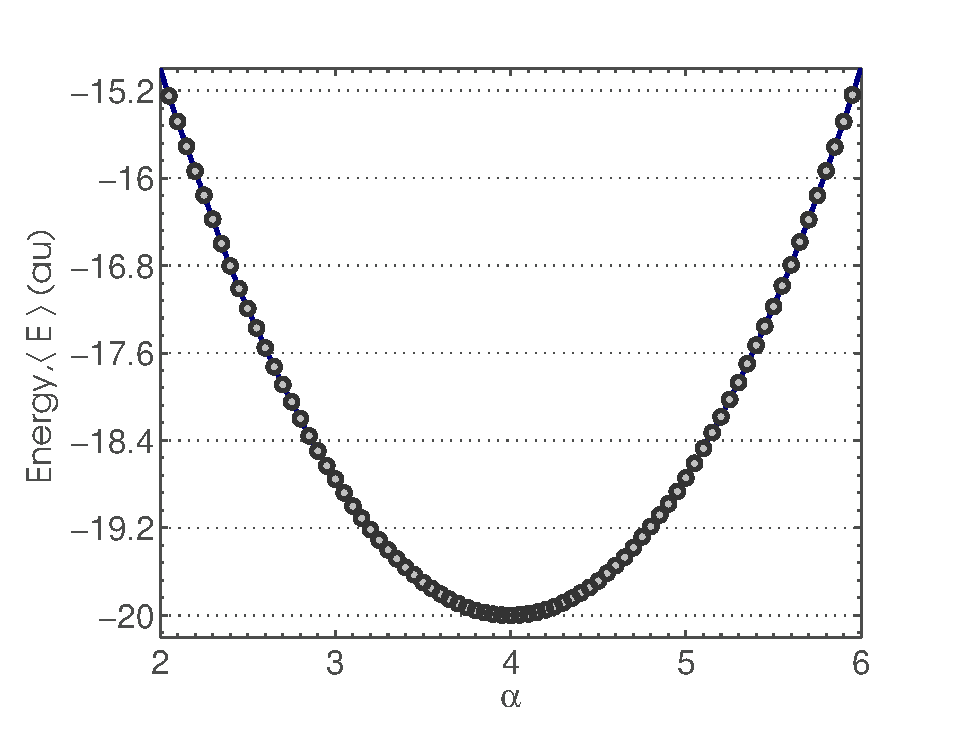
\includegraphics{figures/experimentalData/secondPart/alphaStudy/alphaBe}} \\
% % %        \resizebox{45mm}{!}{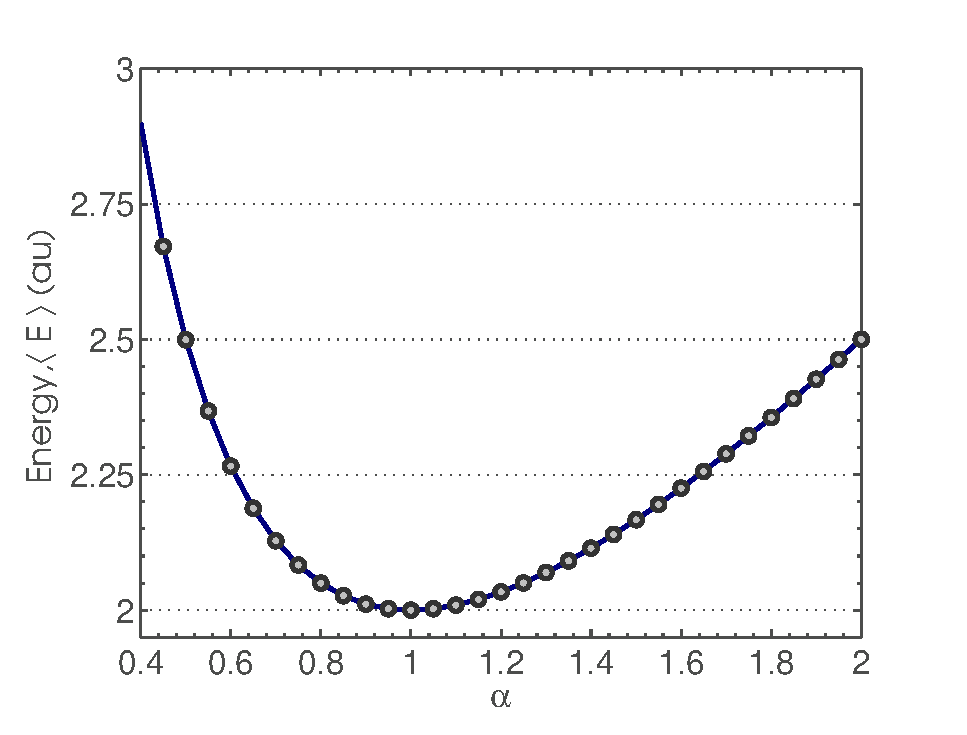
\includegraphics{figures/experimentalData/secondPart/alphaStudy/alpha2DHO2e}} &
% % %       \resizebox{75mm}{!}{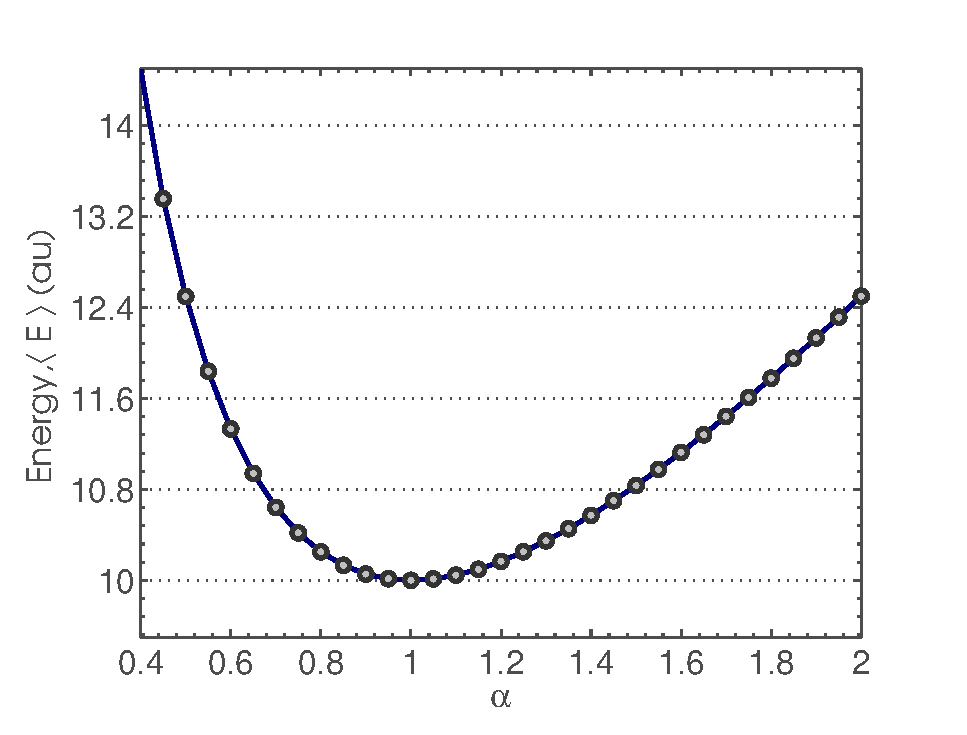
\includegraphics{figures/experimentalData/secondPart/alphaStudy/alpha2DHO6e}}\\      
      \end{tabular}
    \caption{Dependence of the energy on the parameter $\alpha$ for He(left) and Be(right) atoms.}
    \label{alphaHeBe}
  \end{center}
  \end{figure}
\end{frame}


\begin{frame}{Analytical GS for quantum dots (without correlation)}
  \begin{figure}
    \begin{center}
       \begin{tabular}{cc}
      \resizebox{55mm}{!}{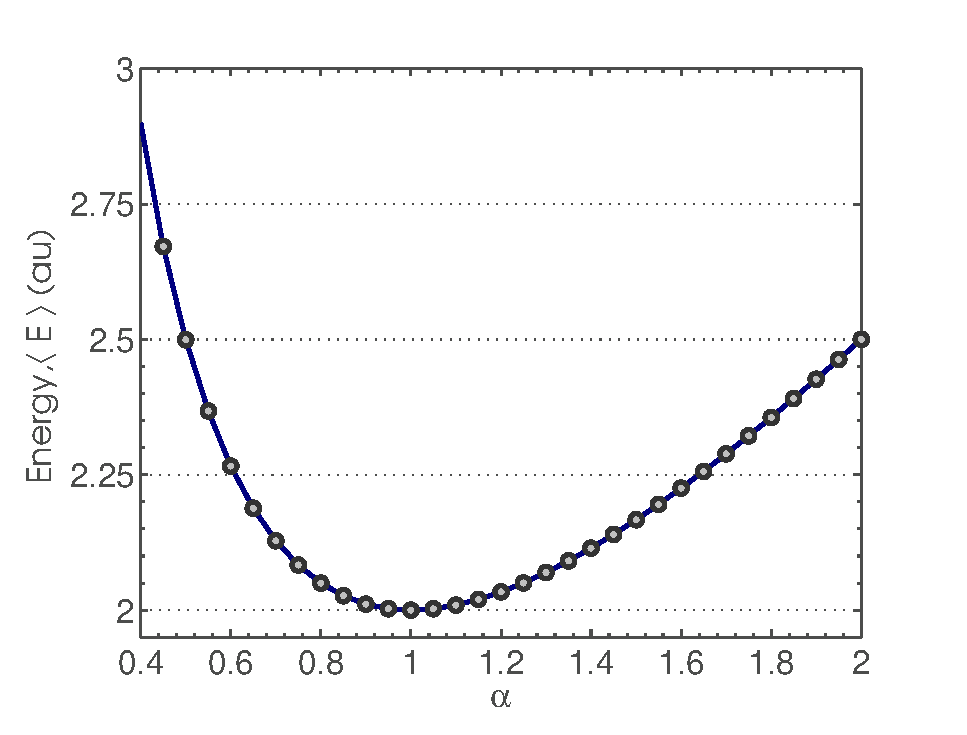
\includegraphics{figures/experimentalData/secondPart/alphaStudy/alpha2DHO2e}} &
      \resizebox{55mm}{!}{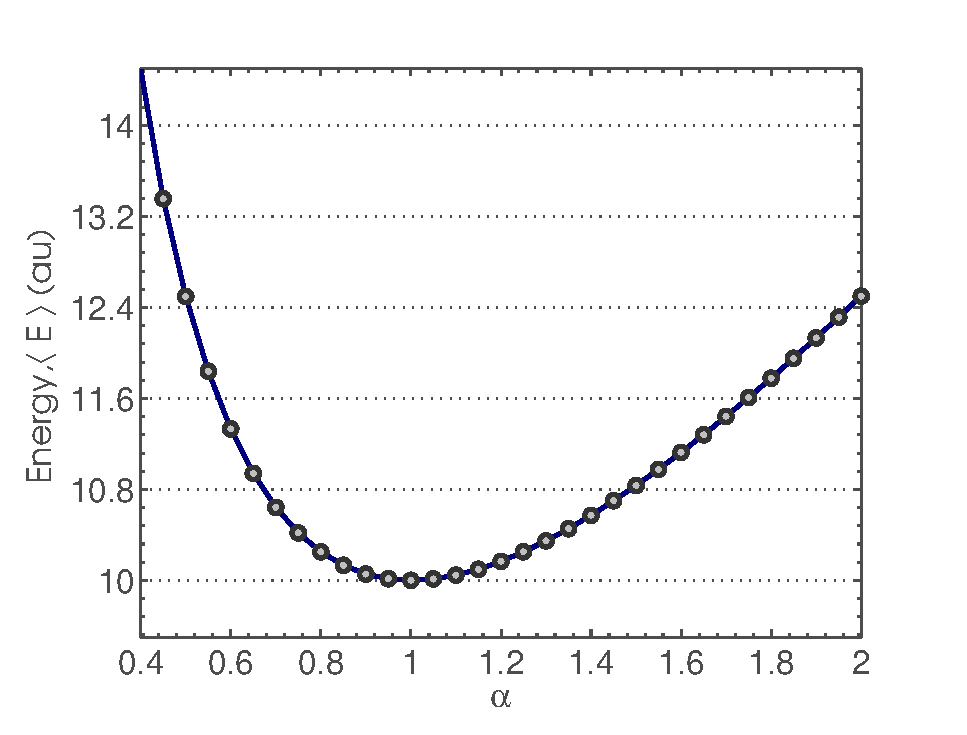
\includegraphics{figures/experimentalData/secondPart/alphaStudy/alpha2DHO6e}}\\
       \end{tabular}
      \caption{Dependence of the energy on the parameter $\alpha$ for a two dimensional harmonic oscillator with two and six electrons electrons, respectively.}
      \label{alpha2DHO2e6e}
    \end{center}
  \end{figure}

\end{frame}



\begin{frame}{Graphical estimation of the GS energy for atoms}
  \begin{figure}[!hbt]
    \begin{center}
      \begin{tabular}{cc}
        \resizebox{55mm}{!}{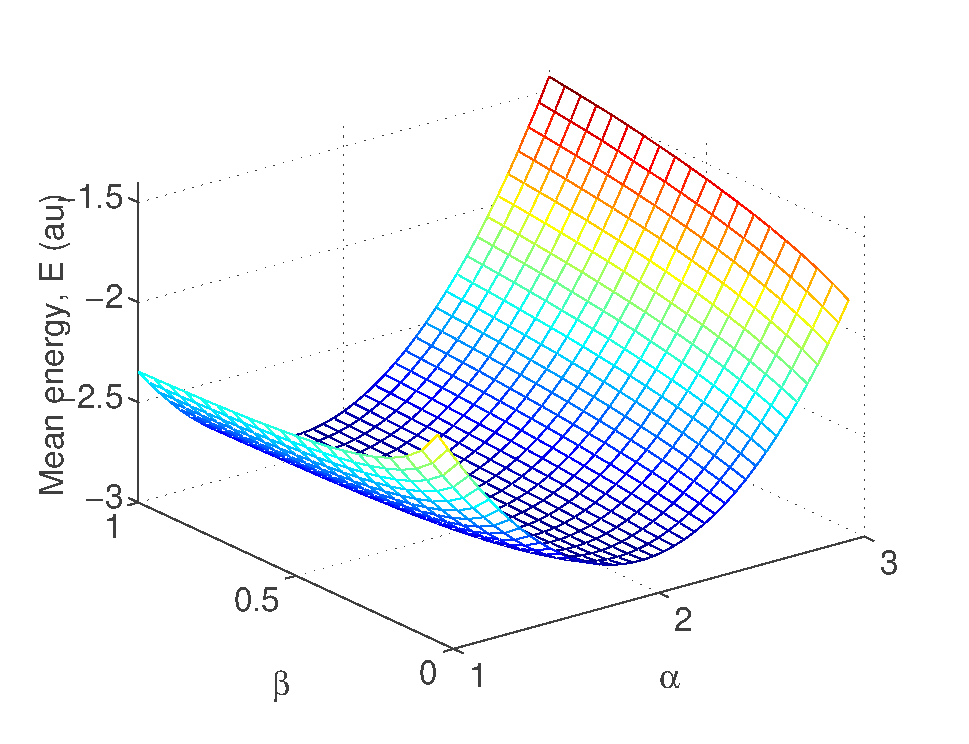
\includegraphics{figures/experimentalData/secondPart/alphaBetaStudy/plot3DAlphaBetaHe}} &
        \resizebox{55mm}{!}{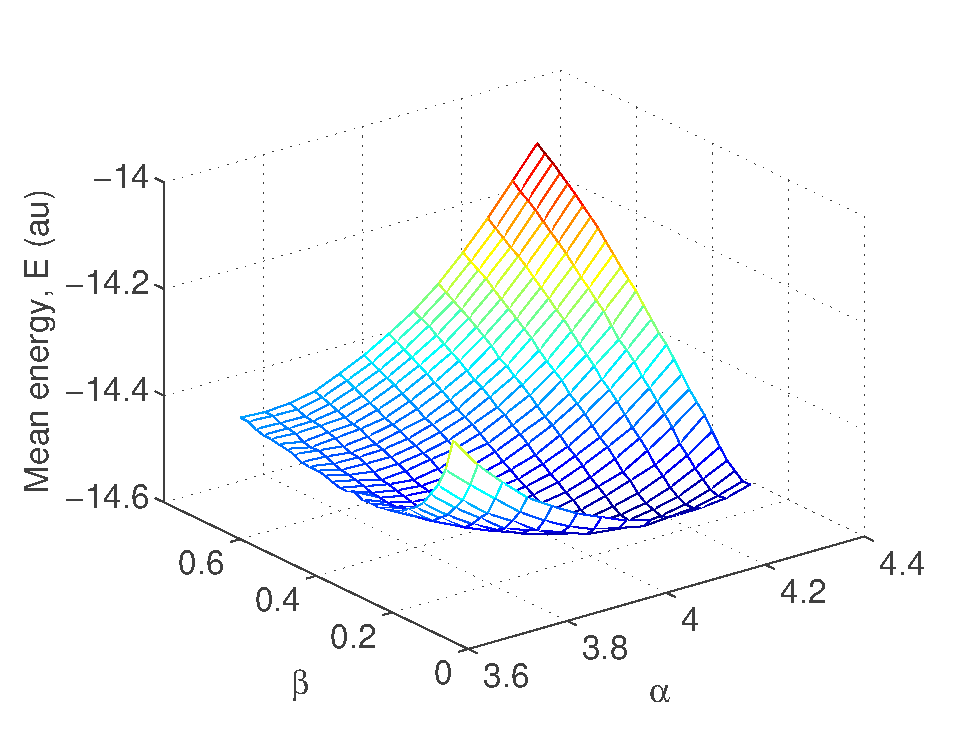
\includegraphics{figures/experimentalData/secondPart/alphaBetaStudy/plot3DAlphaBetaBeSim1}}\\
      \label{alphaBetaHe}
      \end{tabular}
      \caption{Dependence of the energy on the parameters $\alpha$ and $\beta$ for He and Be atoms. Experiment was carried out with $10^7$ Monte Carlo cycles, $10 \%$ equilibration steps and $dt = 0.01$.}
    \end{center}
  \end{figure}
  
\end{frame}



\begin{frame}{Graphical estimation of the GS energy for QD}

  \begin{figure}[!hbt]
    \begin{center}
      \begin{tabular}{cc}
        \resizebox{58mm}{!}{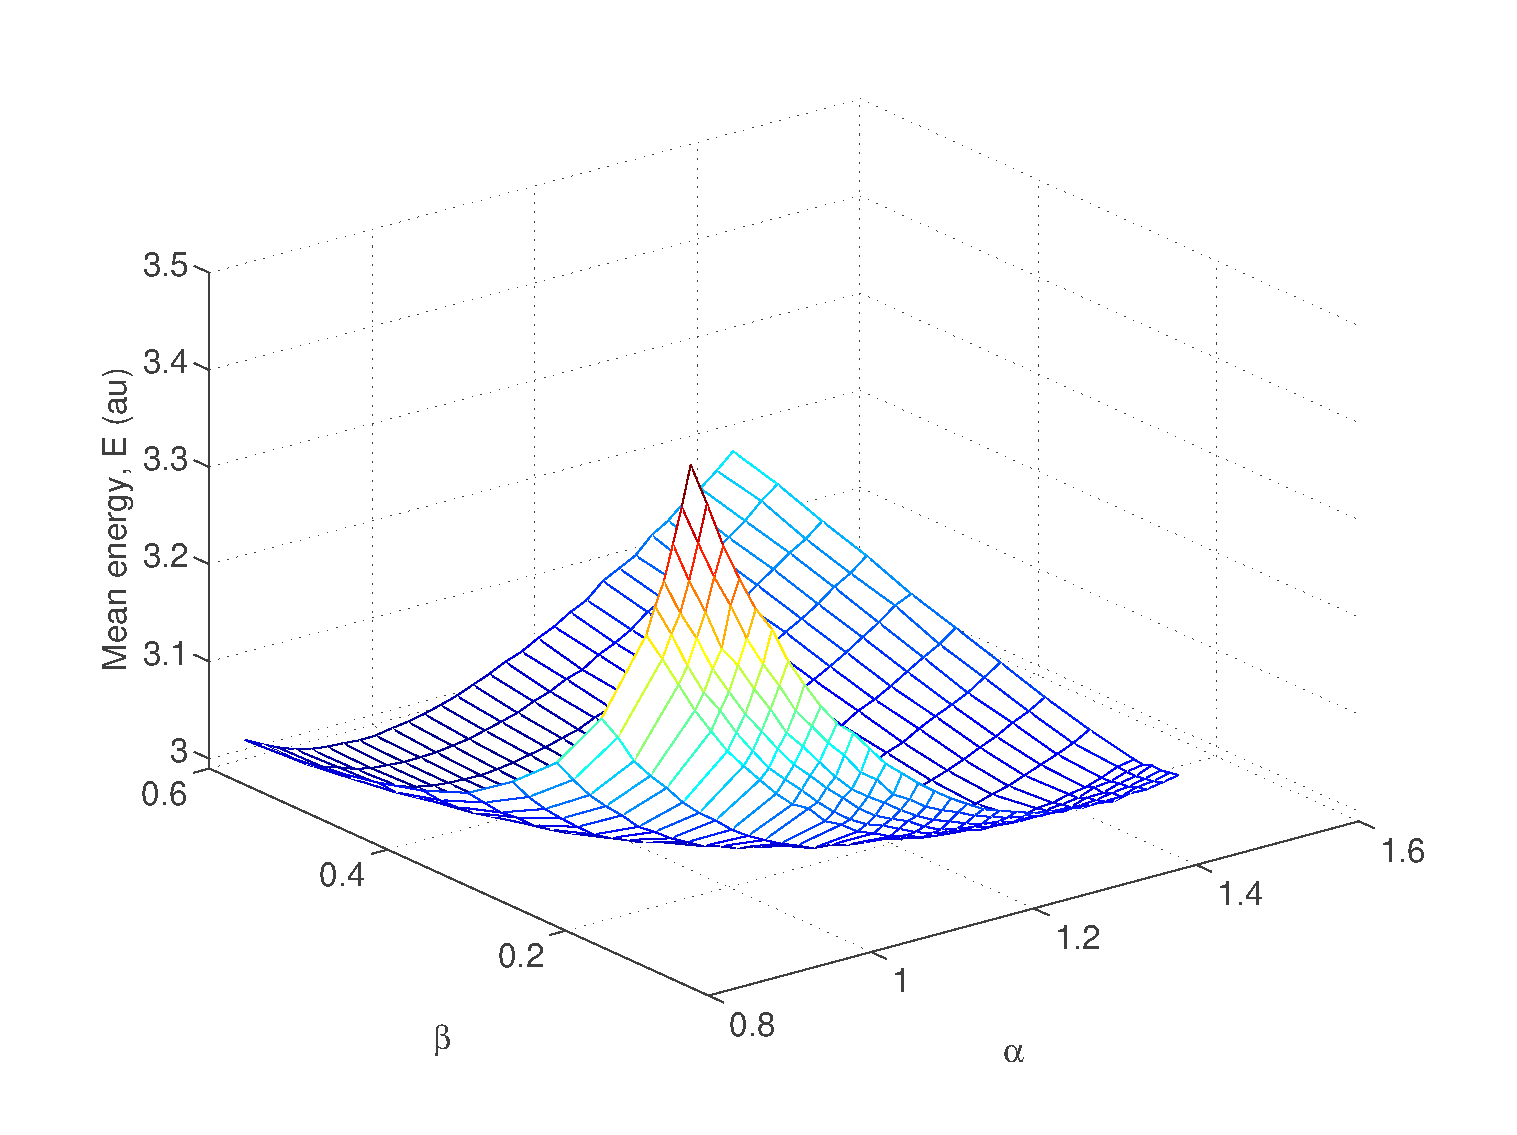
\includegraphics{figures/experimentalData/secondPart/alphaBetaStudy/plotAlphaBeta2DQDot2e}} &
        \resizebox{50mm}{!}{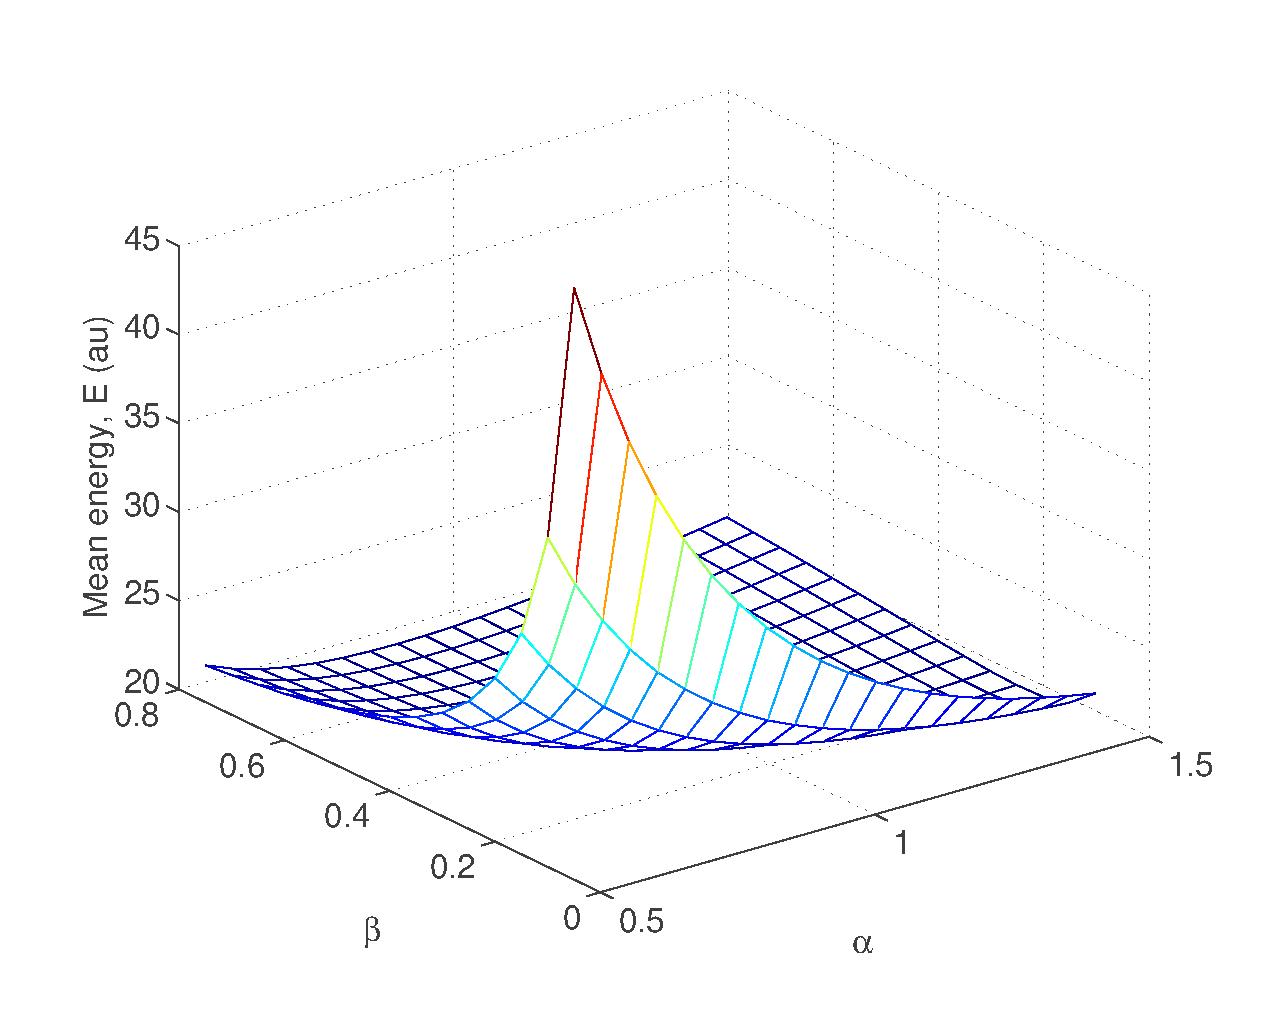
\includegraphics{figures/experimentalData/secondPart/alphaBetaStudy/alphaBeta}} \\
        \label{alphaBetaHe}
        \end{tabular}
       \caption{Dependence of the energy on the parameters $\alpha$ and $\beta$ for a two-dimensional quantum dots with two and electrons, respectively. Experiment was carried out with $10^7$ Monte Carlo cycles, $10 \%$ equilibration steps and $dt = 0.01$.}
    \end{center}
  \end{figure}
 
\end{frame}

  
\begin{frame}{Graphical estimation of the GS energy for helium}  
  \begin{scriptsize}
  \begin{figure}[!hbt]
    \begin{center}
       \begin{tabular}{cc}
      \resizebox{55mm}{!}{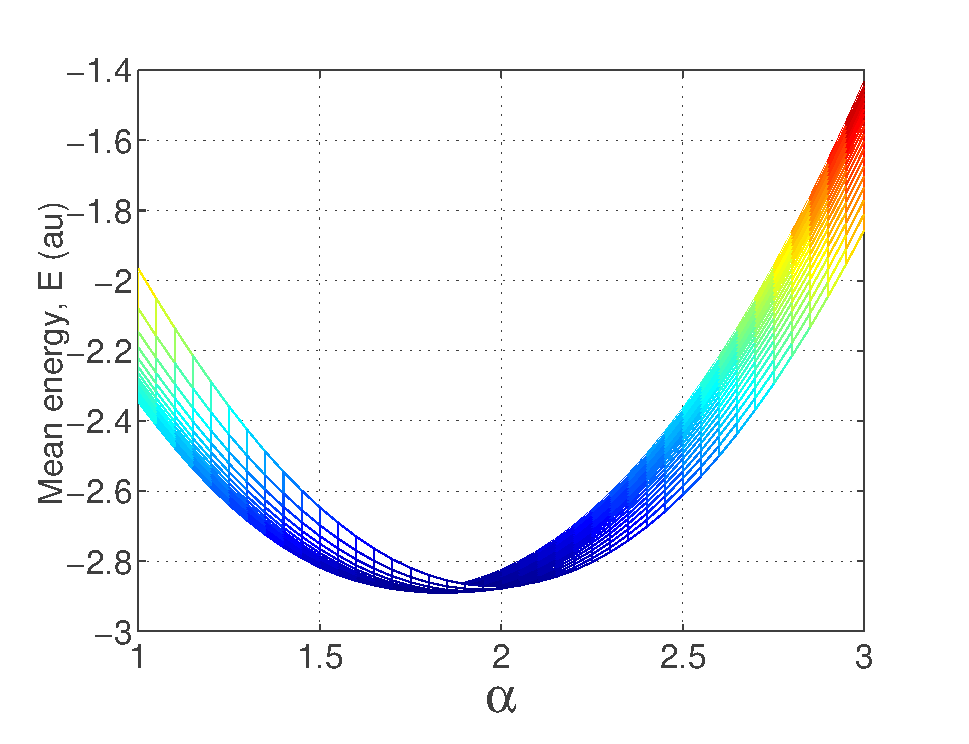
\includegraphics{figures/experimentalData/secondPart/alphaBetaStudy/zoomAlphaHe}}&%%%alphaBetaStudies/alphaZoomHe}} &
      \resizebox{55mm}{!}{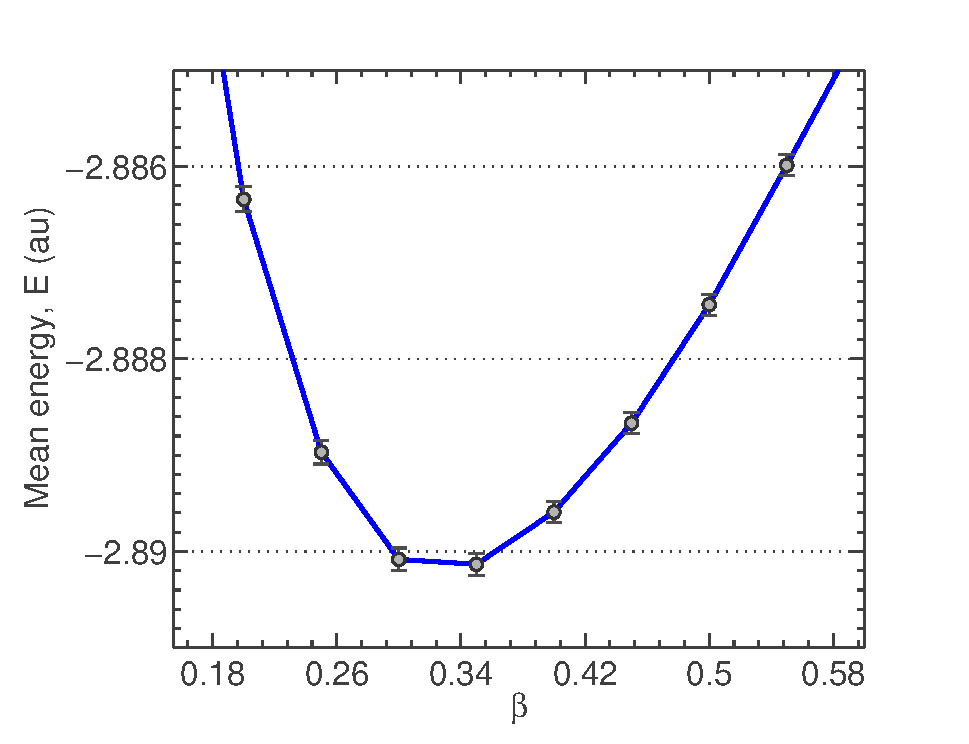
\includegraphics{figures/experimentalData/secondPart/alphaBetaStudy/minBetaFixedAlphaHe}}\\%%%%alphaBetaStudies/minBetaHeFixedAlpha1_85}}\\
       \end{tabular}
      \caption{Dependence of the energy on $\alpha$ (left) along the value of $\beta$ (right) that gives the minimum variational energy for a He atom.}
      \label{alphaHe}
    \end{center}
  \end{figure}
  \end{scriptsize}

\end{frame}





\begin{frame}{Graphical estimation of the GS energy for beryllium}
  \begin{figure}[!hbt]
  \begin{center}
    \begin{tabular}{cc}
      \resizebox{55mm}{!}{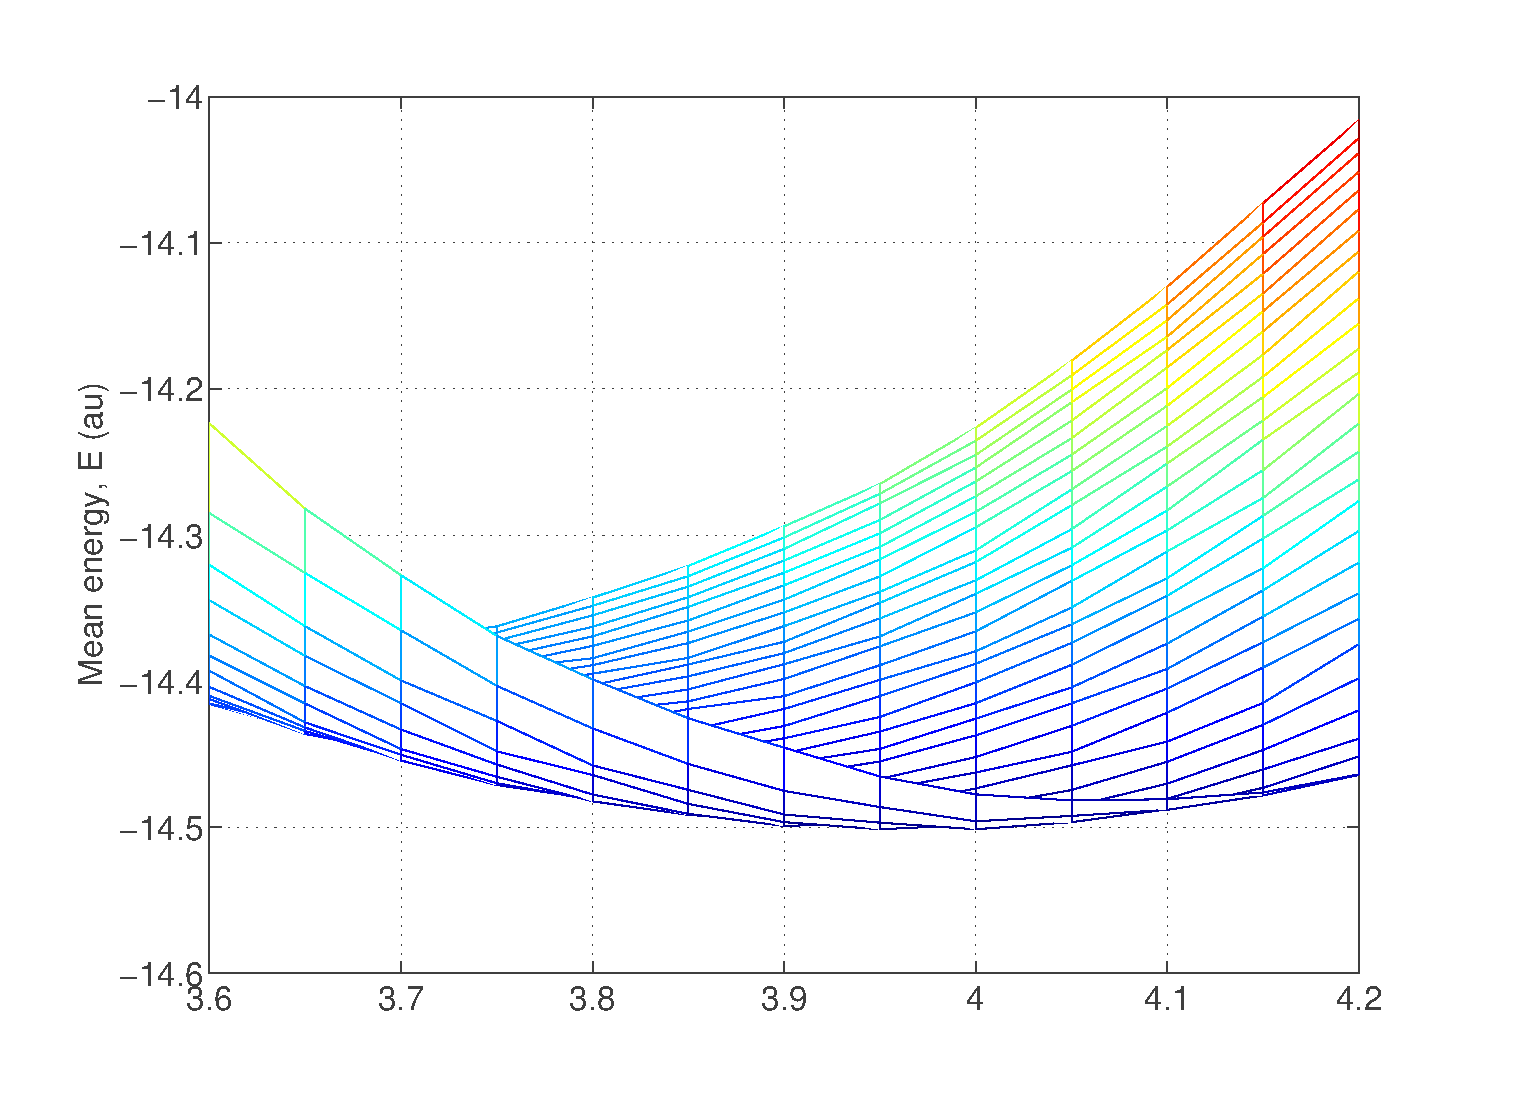
\includegraphics{figures/experimentalData/secondPart/alphaBetaStudy/zoomAlphaBeSim1}}&
      \resizebox{55mm}{!}{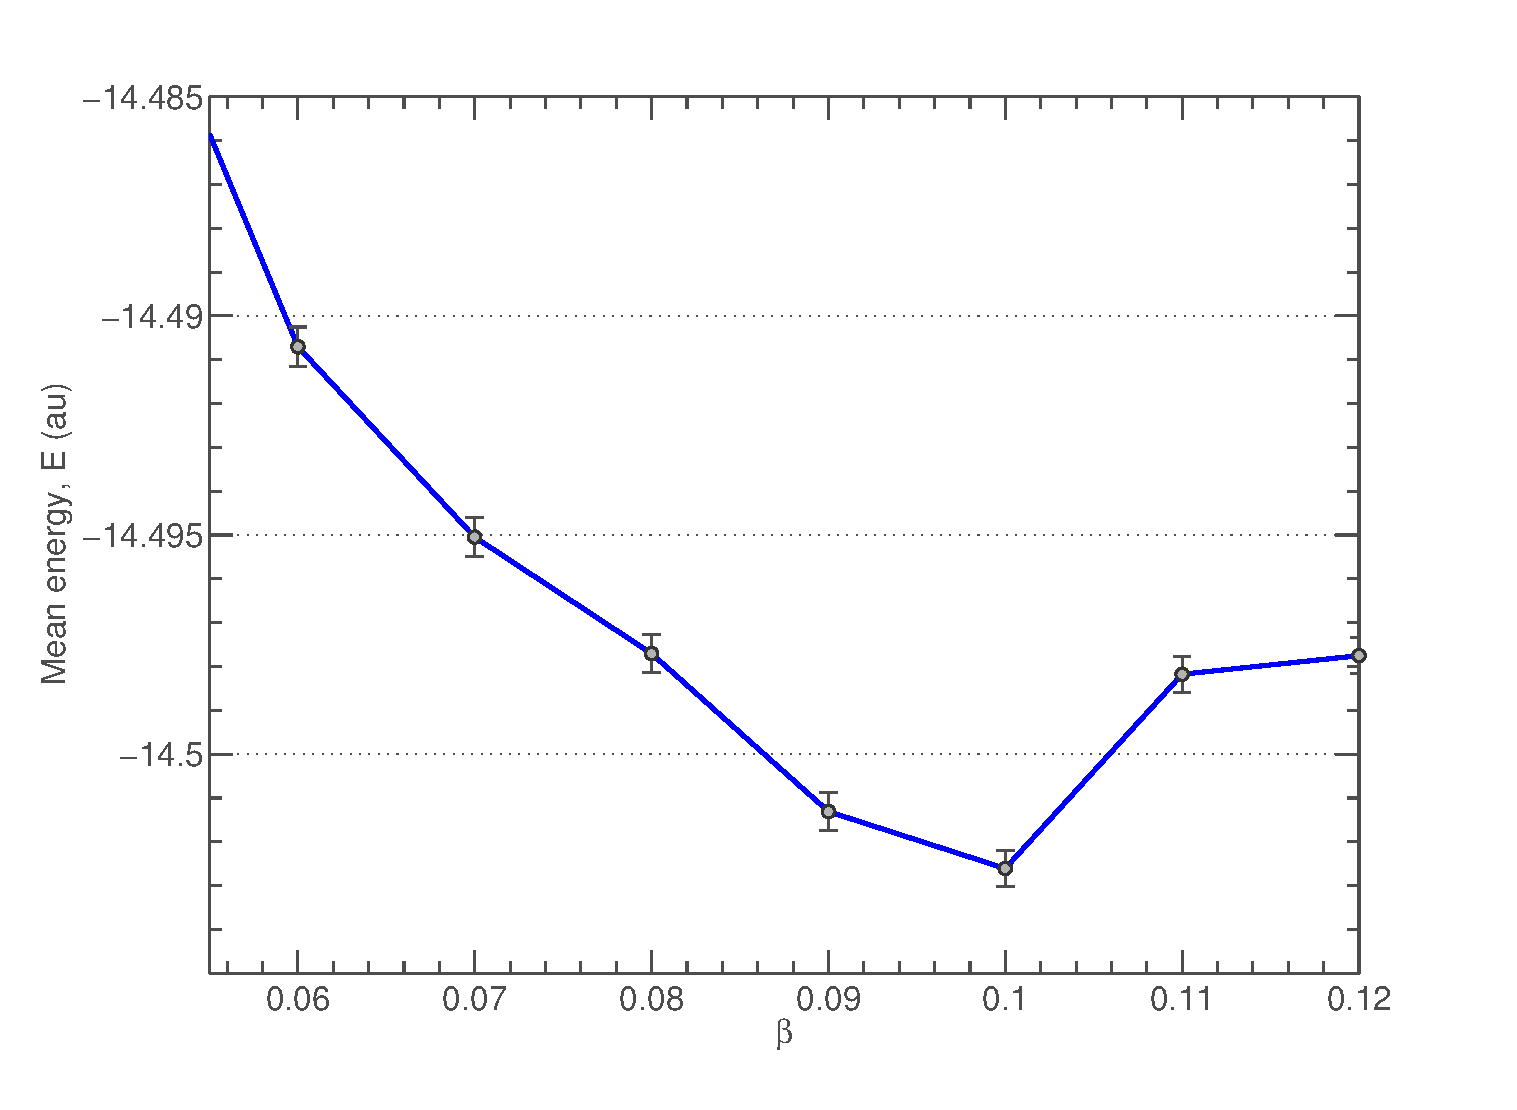
\includegraphics{figures/experimentalData/secondPart/alphaBetaStudy/minBetaFixedAlphaBeSim2}}\\
    \end{tabular}
    \caption{Dependence of the energy on $\alpha$ (left) along the value of $\beta$ (right) that gives the minimum variational energy for a Be atom.}
  \end{center}
  \end{figure}
\end{frame}




\begin{frame}{Graphical estimation of the GS energy for 2-$e^-$ QD}
  \begin{figure}[!hbt]
    \begin{center}
       \begin{tabular}{cc}
        \resizebox{55mm}{!}{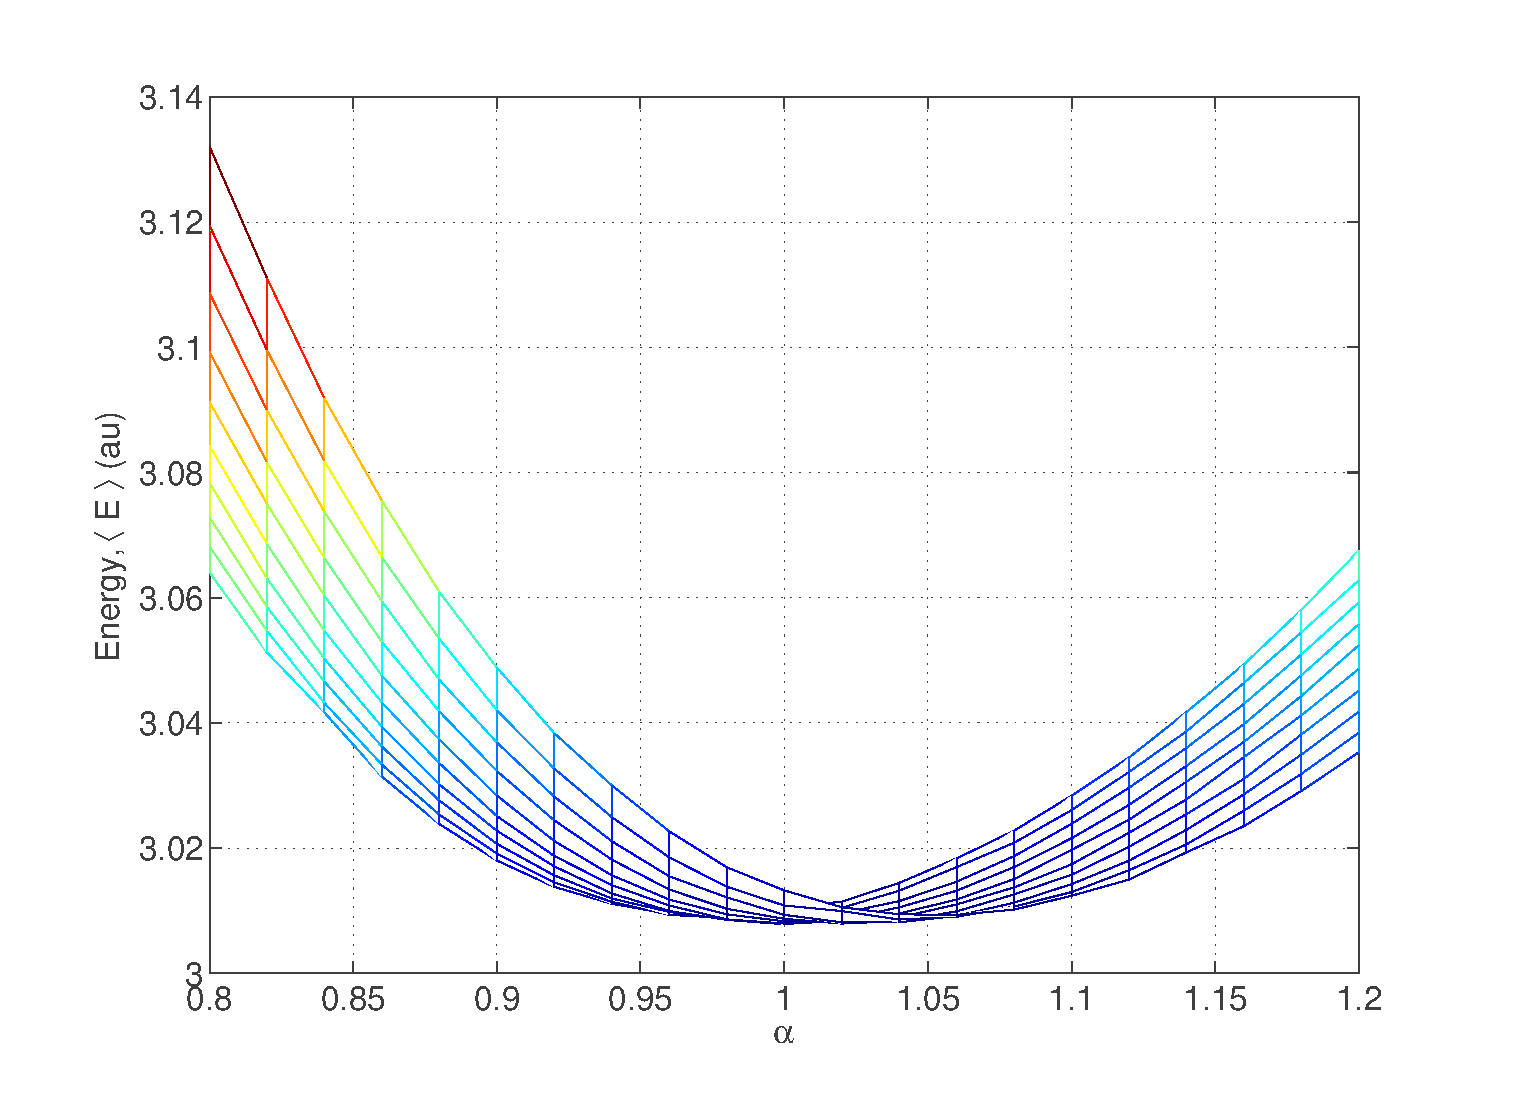
\includegraphics{figures/experimentalData/secondPart/alphaBetaStudy/zoomAlpha2DQDot2e}} &
        \resizebox{55mm}{!}{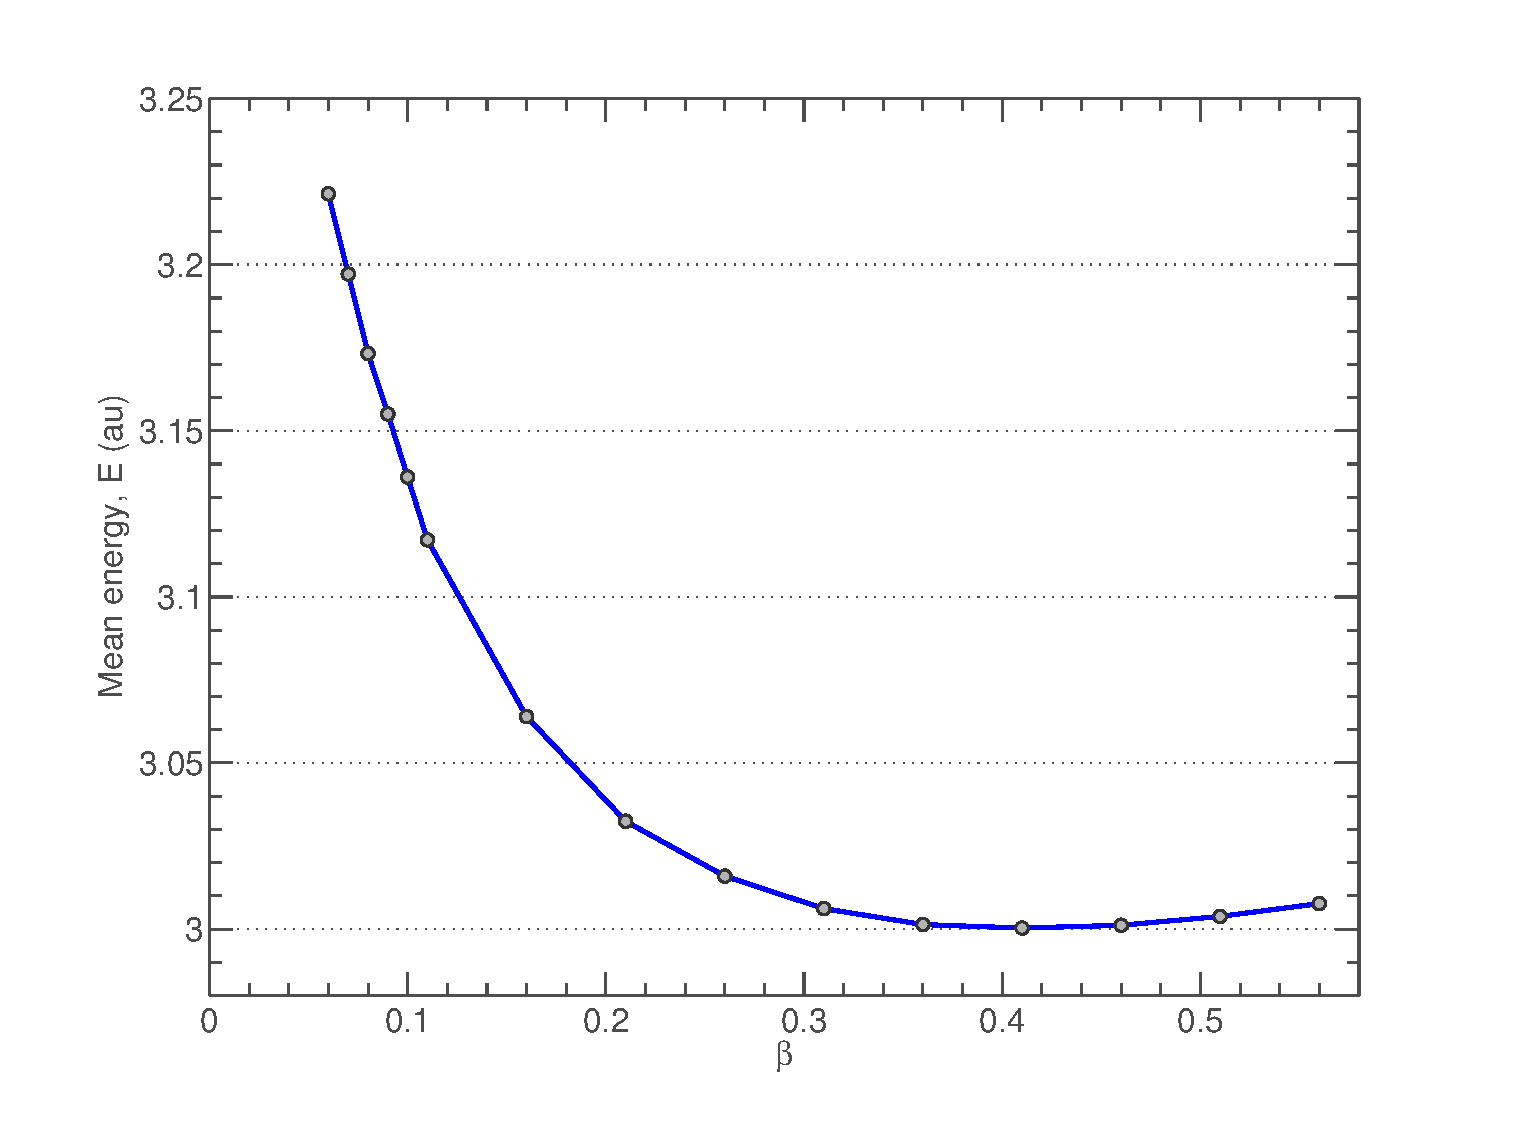
\includegraphics{figures/experimentalData/secondPart/alphaBetaStudy/zoomBeta2DQDot2e}}\\
      \end{tabular}
      \caption{Dependence of the energy on $\alpha$ (left) along the value of $\beta$ (right) that gives the minimum variational energy for a two-dimensional quantum dot with two electrons.}
      \label{alpha2DHO2e}
    \end{center}
  \end{figure}
\end{frame}


\begin{frame}{Graphical estimation of the GS energy for 6-$e^-$ QD}
  \begin{figure}[!hbt]
    \begin{center}
       \begin{tabular}{cc}
      \resizebox{55mm}{!}{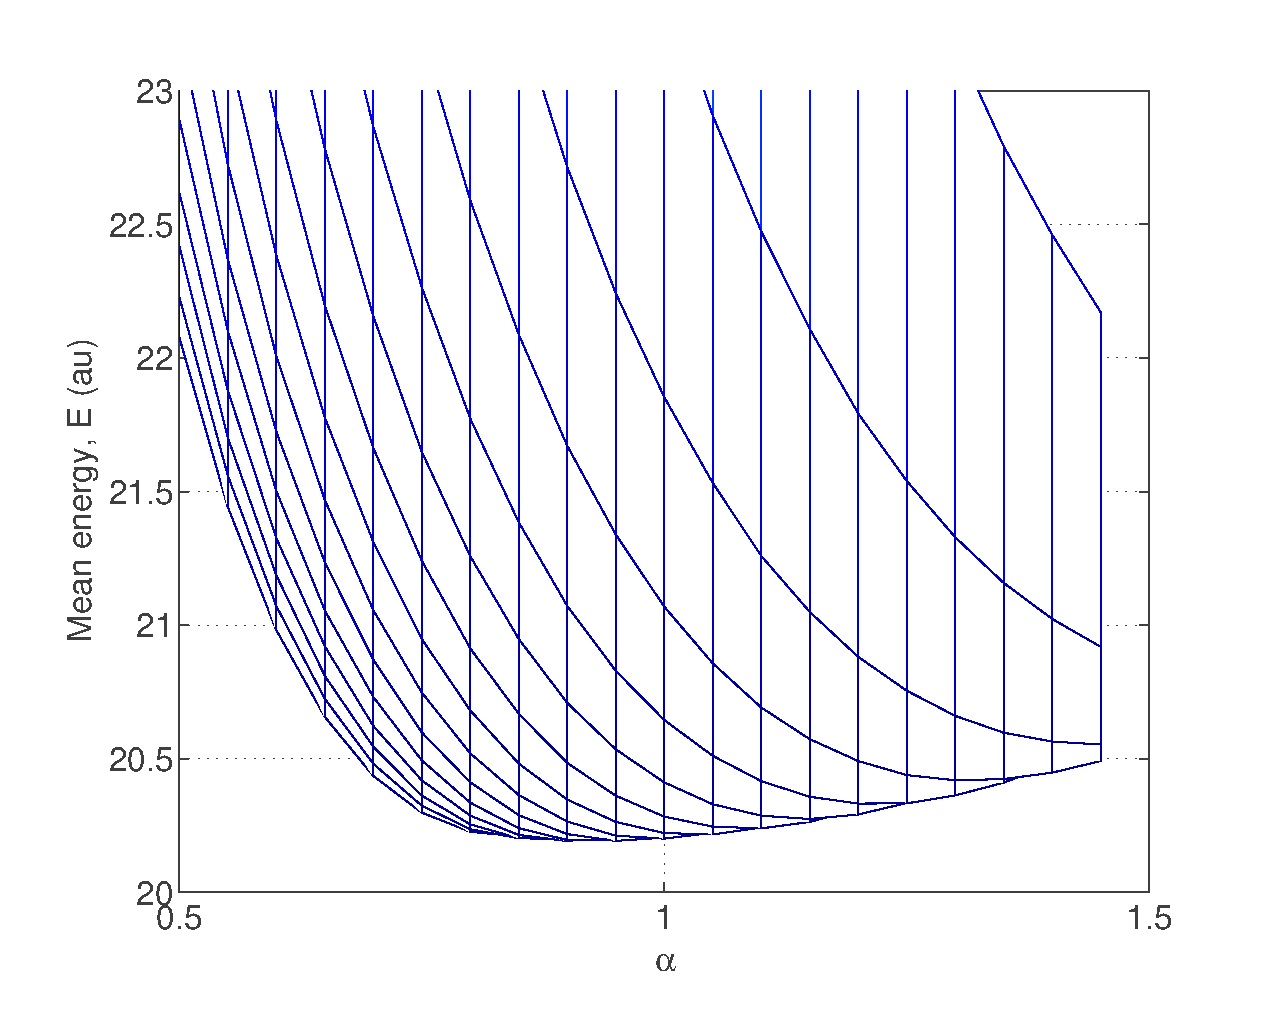
\includegraphics{figures/experimentalData/secondPart/alphaBetaStudy/zoomAlpha}} &
      \resizebox{55mm}{!}{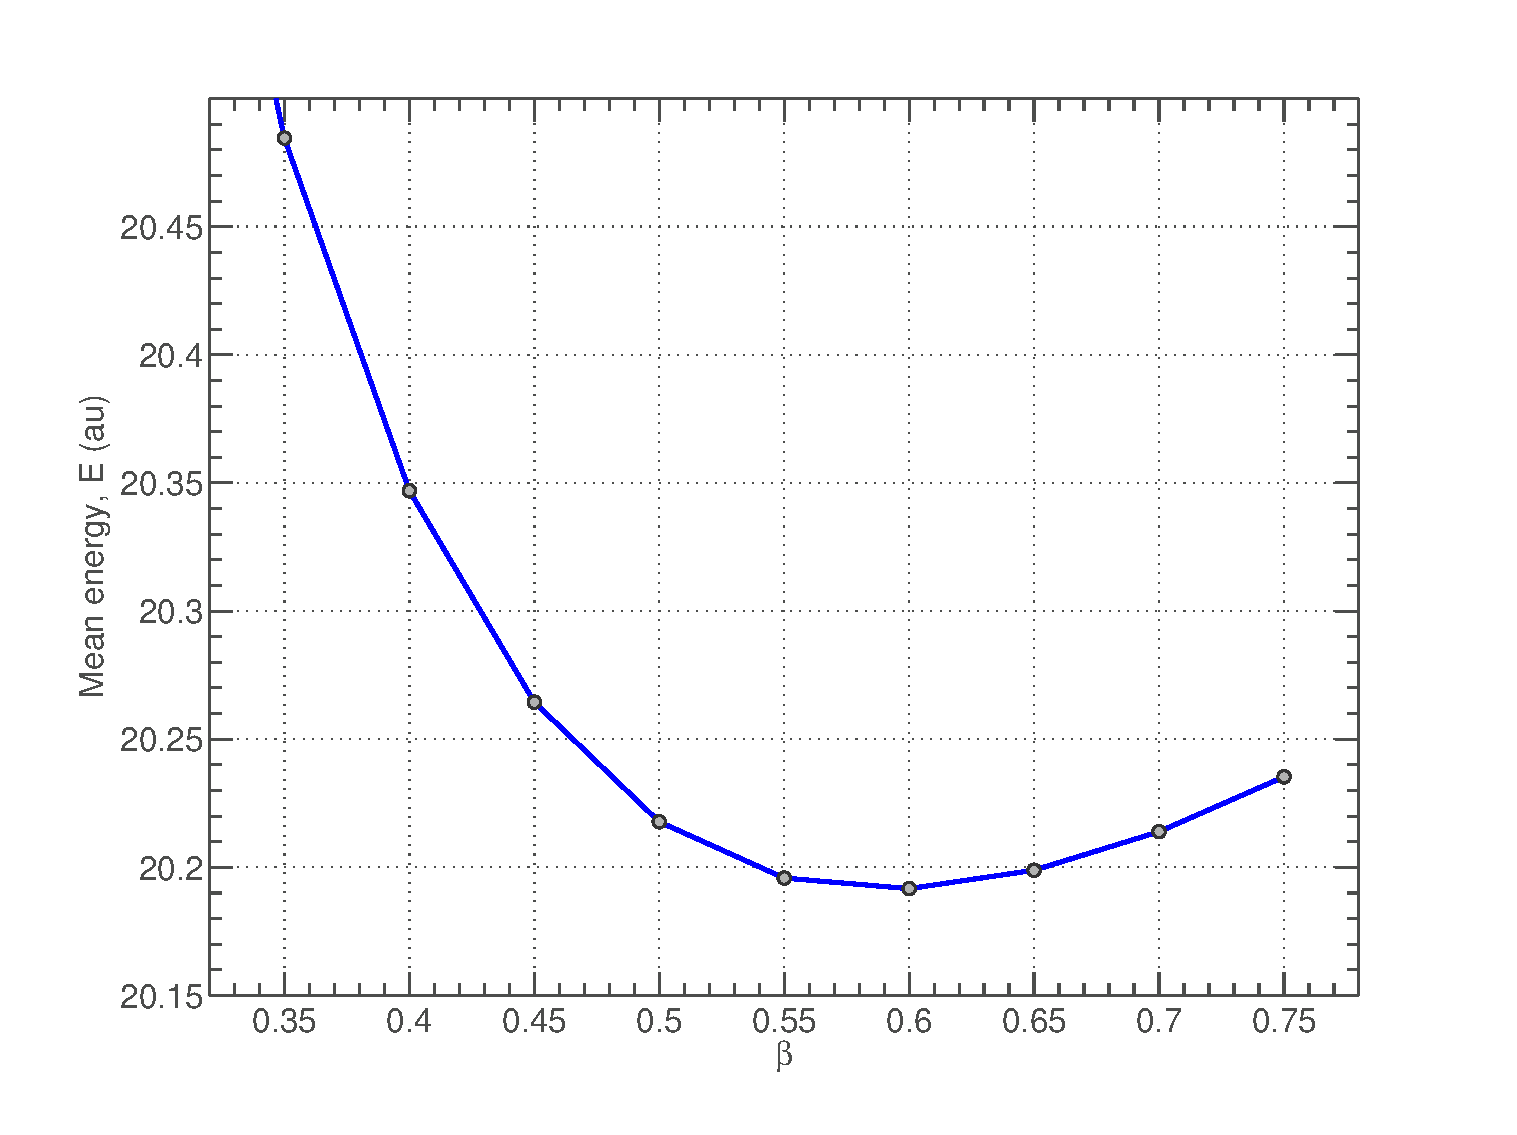
\includegraphics{figures/experimentalData/secondPart/alphaBetaStudy/zoomBeta}}\\
       \end{tabular}
      \caption{Dependence of the energy on $\alpha$ (left) along the value of $\beta$ (right) that gives the minimum variational energy for a two-dimensional quantum dot with six electrons.}
      \label{alpha2DHO6e}
    \end{center}
  \end{figure}

\end{frame}

\begin{frame}{Summary of the results with graphical estimation}
  \begin{scriptsize}
  \begin{table}[!hbt]
  \centering
    \begin{tabular}{lcccr}
      \toprule[1pt]
      \textbf{System} & $\alpha_{optimal}$ & $\beta_{optimal}$ & \textbf{Energy}, $\langle E \rangle$ (au) \\
      \midrule[1pt]
      He      &  1.85   &   0.35  & $-2.8901 \pm 1.0 \times 10{-4}$ \\
      Be      &  3.96   &   0.09  & $-14.5043 \pm 4.0 \times 10^{-4}$\\
      2DQDot2e ($\omega=1.0$) & 0.98  & 0.41  & $3.0003 \pm 1.2 \times 10^{-5}$ \\
      %%%2DQDot6e ($\omega = 1.0$)  & 1.03   & 0.18 & $20.2180 \pm 4.0 \times 10^{-4}$\\
      2DQDot6e ($\omega = 1.0$) & 0.9   & 0.6 & $20.19 \pm 1.2 \times 10^{-4}$\\
      \bottomrule[1pt]
    \end{tabular}\caption{Ground state energy and corresponding variational parameters  $\alpha$ and $\beta$ estimated graphically. (2DQDot2e stands for two-dimensional quantum dot with two electrons).}
    \label{energiesWithGraphPar}
  \end{table}
  \end{scriptsize}
\end{frame}

\subsection{Optimization of the trial wave function}
\begin{frame}{Optimization with Quasi-Newton method}

  \begin{scriptsize}
  \begin{table}[!hbt]
  \centering
  \begin{tabular}{lccccrcc}
    \toprule[1pt]
    \textbf{System} & $\alpha_{0}$ & $\beta_{0}$ & $\alpha_{opt}$ & $\beta_{opt}$ &\textbf{Energy}, (au)\\
    \midrule[1pt]
    He              & 1.564  & 0.134    & 1.838   &  0.370  & -2.891   \\
    Be              & 3.85  & 0.08    & 3.983   &  0.104  &   -14.503  \\
    \bottomrule[1pt]
  \end{tabular}\caption{Optimized variational parameters and corresponding energy minimization using a quasi-Newton method. Simulation parameters: $10^7$ Monte Carlo cycles with 10 \% equilibration steps, $dt = 0.01$.}\label{optizedQuasiNewtonParameters}
  \end{table}
  \end{scriptsize}

\end{frame}




\begin{frame}{Convergence to the optimal parameters for helium}
  \begin{scriptsize}
  \begin{figure}[!hbt]
    \begin{center}
      \begin{tabular}{cc}
        \resizebox{50mm}{!}{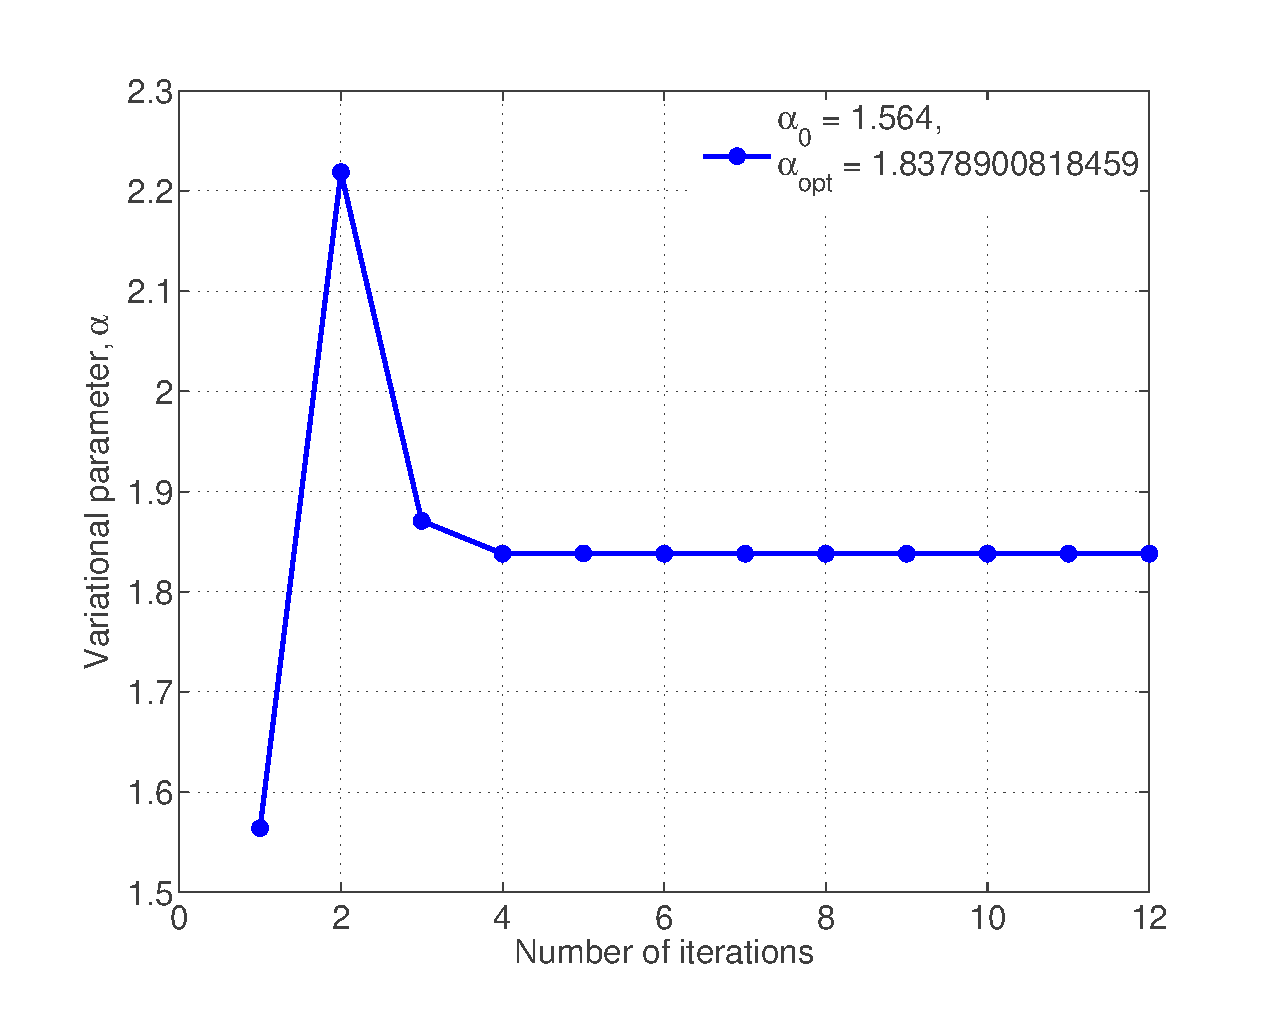
\includegraphics{figures/experimentalData/quasiNewtonOptimization/plotAlphaEvolHe}}&
        \resizebox{50mm}{!}{\includegraphics{figures/experimentalData/quasiNewtonOptimization/plotBetaEvolHe}}\\
      \end{tabular}
      \caption{Evolution of the variational parameters $\alpha$ and $\beta$ as a function of the number of iterations during the optimization of the trial wave function of He atom with quasi-Newton method. The experiment was carried out with $10^7$ Monte Carlo cycles and $10 \%$ equilibration steps in four nodes.}
    \end{center}
  \end{figure}
  \end{scriptsize}  
\end{frame}




\begin{frame}{Convergence to the minimal energy for helium}
  \begin{scriptsize}
  \begin{figure}[!hbt]
    \begin{center}
      \resizebox{60mm}{!}{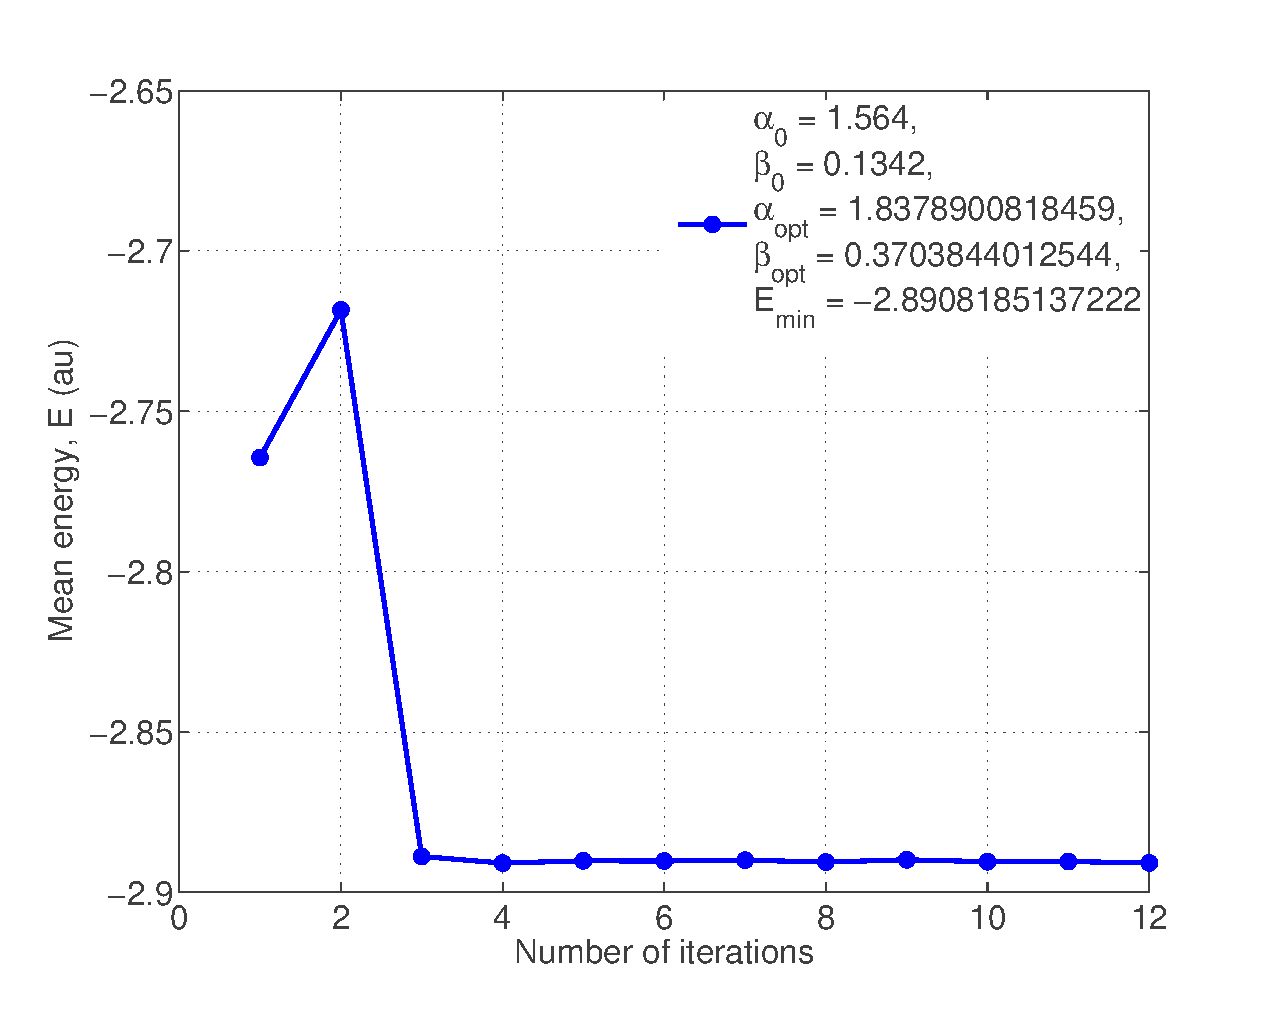
\includegraphics{figures/experimentalData/quasiNewtonOptimization/plotOptAlphaBetaEnergyHe}}\\
      \caption{Evolution of the energy as a function of the number of iterations during the optimization of the trial wave function of He atom with the quasi-Newton method. The experiment was carried out with $10^7$ Monte Carlo cycles and $10 \%$ equilibration steps in four nodes.}
      \label{quasiNewtonOptHe}
    \end{center}
  \end{figure}
  \end{scriptsize}
\end{frame}




\begin{frame}{Convergence to the optimized parameters for Be}
  \begin{scriptsize}
  \begin{figure}[!hbt]
  \begin{center}
    \begin{tabular}{cc}
      \resizebox{55mm}{!}{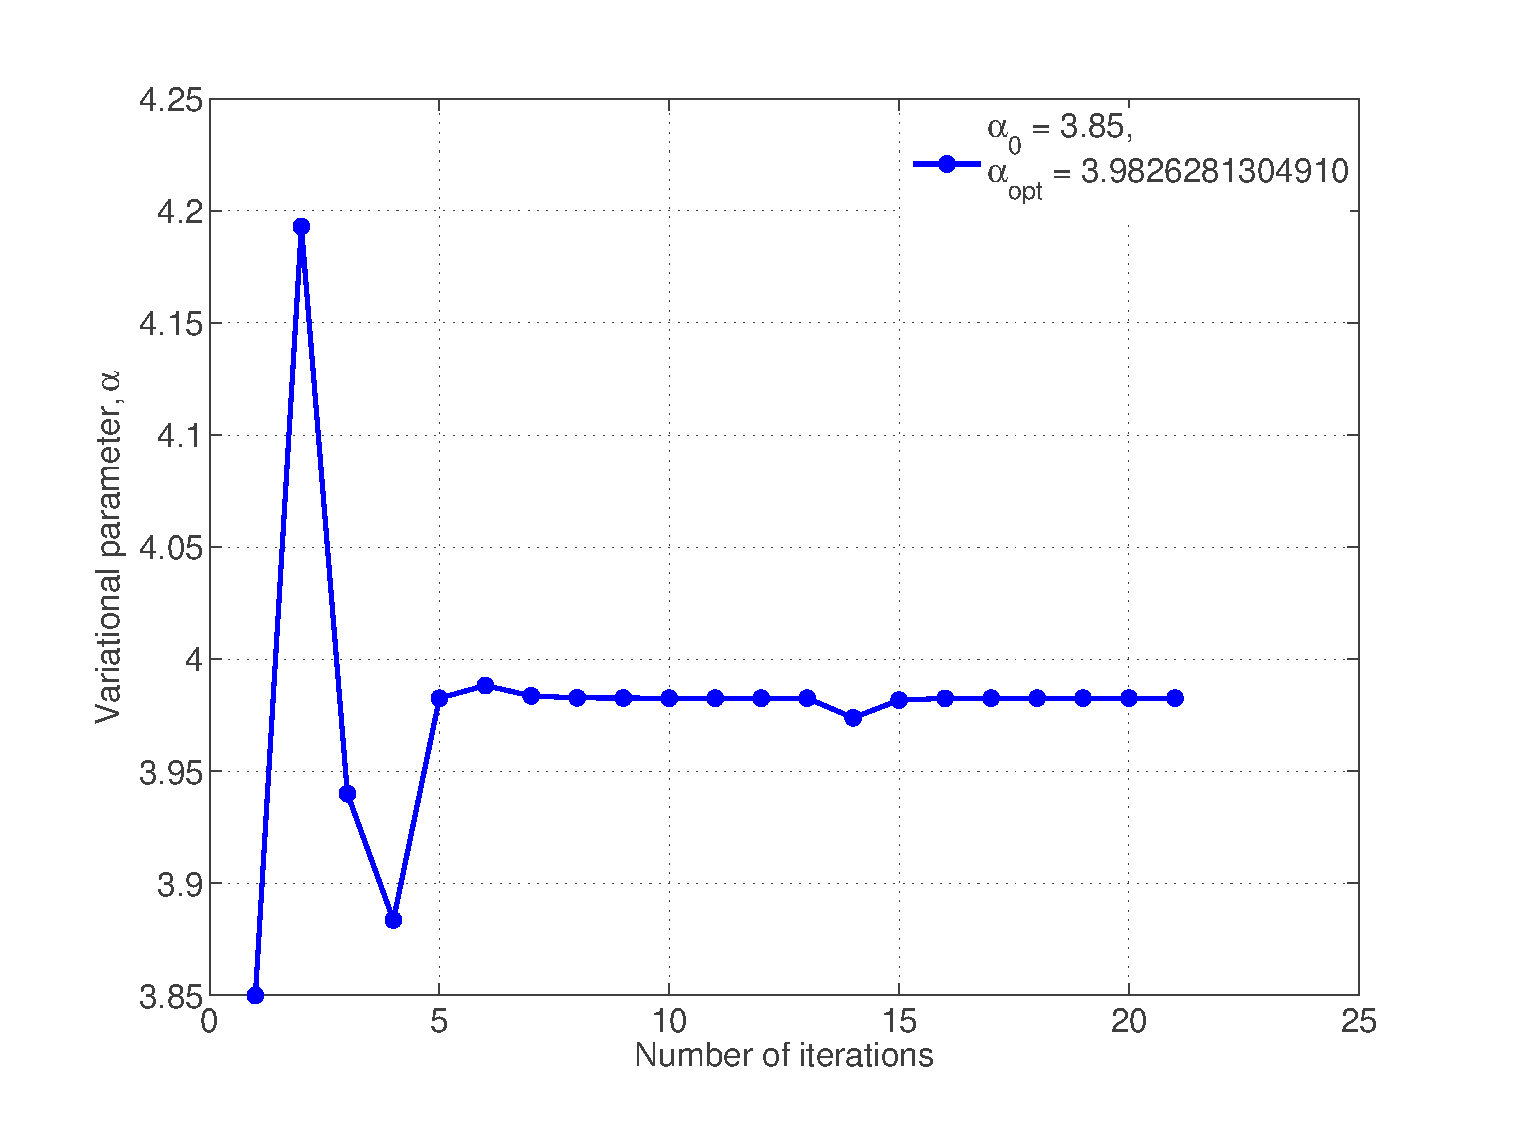
\includegraphics{figures/experimentalData/quasiNewtonOptimization/evolAlphaBeOpt}}&
      \resizebox{55mm}{!}{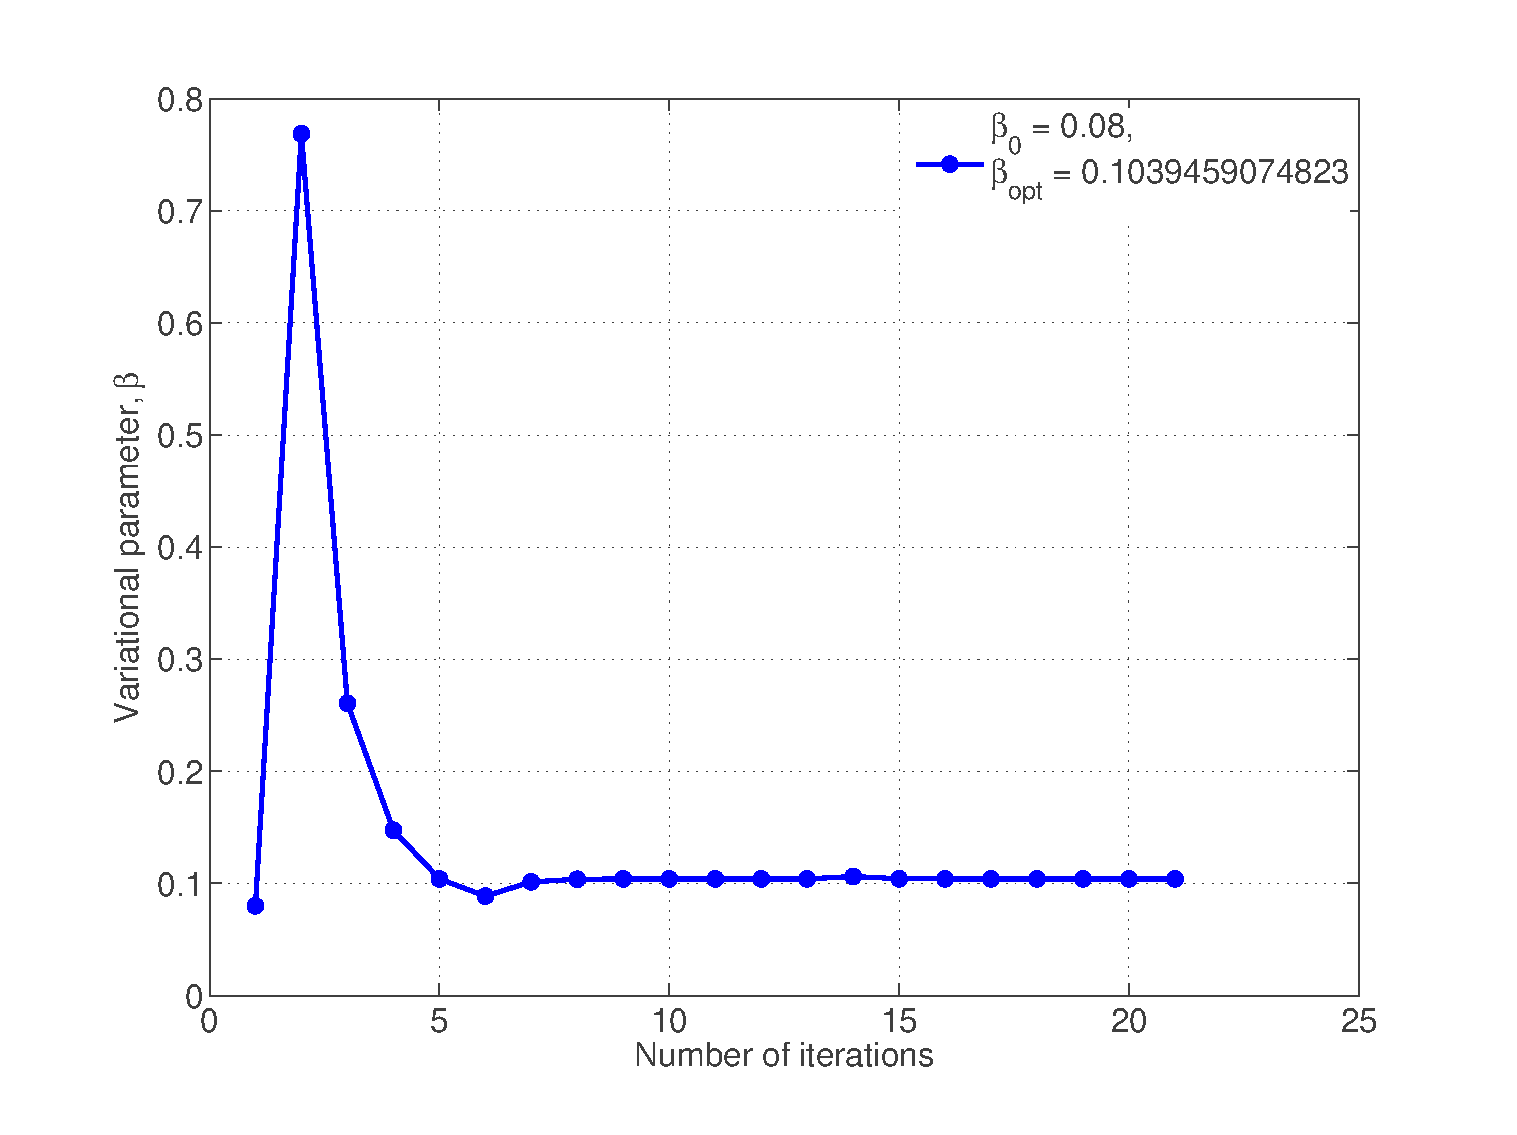
\includegraphics{figures/experimentalData/quasiNewtonOptimization/evolBetaBeOpt}}\\
    \end{tabular}
    \caption{Evolution of the variational parameters $\alpha$ and $\beta$ with the number of iterations during the optimization of the trial wave function of Be atom with the quasi-Newton method. The experiment was carried out with $10^7$ Monte Carlo cycles and $10 \%$ equilibration steps in four nodes.}
    \label{quasiNewtonOptBe}
  \end{center}
  \end{figure}
  \end{scriptsize}
\end{frame}




\begin{frame}{Convergence to the minimal energy for Be}
  \begin{scriptsize}
  \begin{figure}[!hbt]
  \begin{center}
    \resizebox{60mm}{!}{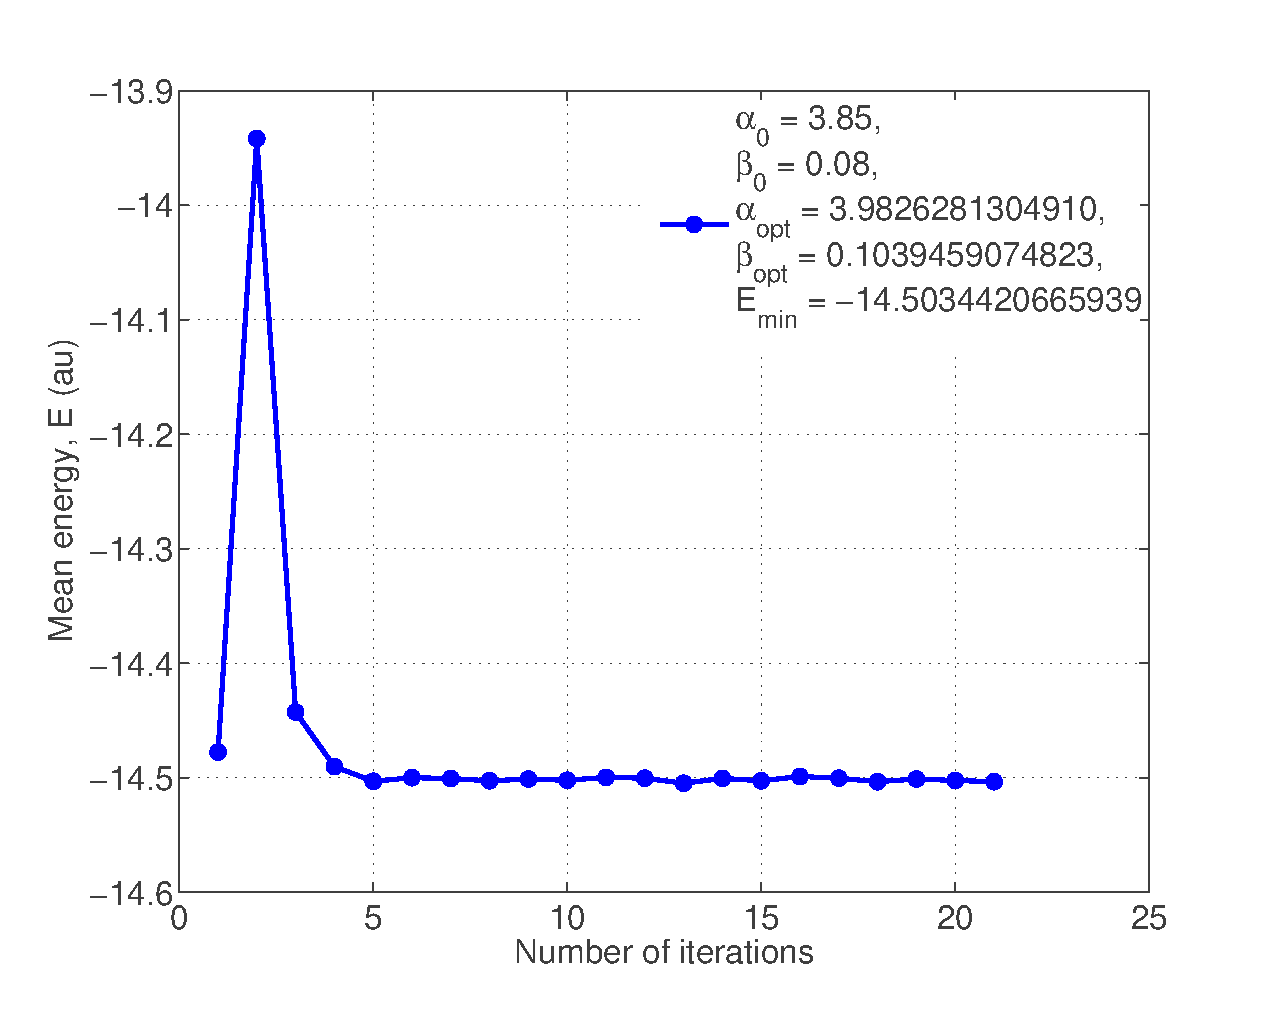
\includegraphics{figures/experimentalData/quasiNewtonOptimization/plotEnergyOptimizationBe}}\\
    \caption{Evolution of the energy with the number of iterations during the optimization of the trial wave function of Be atom with the quasi-Newton method. The experiment was carried out with $10^7$ Monte Carlo cycles and $10 \%$ equilibration steps in four nodes.}
    \label{quasiNewtonOptBe}
  \end{center}
  \end{figure}
  \end{scriptsize}
\end{frame}



%%%%%%%%%%%%%%% GROUND STATE ENERGIES %%%%%%%%%%%%%%%%%%%%%%
%%%%%%%%%%%%%%%%%%%%%%%%%%%%%%%%%%%%%%%%%%%%%%%%%%%%%%%%%%%%
\subsection{Extrapolation to zero dt}
\begin{frame}{Extrapolation of energy to zero dt for He}

  \begin{scriptsize}
  \begin{table}[!hbt]
  \centering
  \begin{tabular}{cccc}
    \toprule[1pt]
    \textbf{Time step} & \textbf{Energy}, (au)  & \textbf{Error} & \textbf{Accepted moves}, (\%) \\
    \midrule[1pt]
    0.002  & -2.891412637854  &  5.5e-4   &  99.97\\
    0.003  & -2.890797649433  &  4.5e-4   &  99.94\\
    0.004  & -2.890386198895  &  4.0e-4   &  99.91\\
    0.005  & -2.890078440930  &  3.5e-4   &  99.88\\
    0.006  & -2.890463490951  &  3.2e-4   &  99.84\\
    0.007  & -2.890100432462  &  2.8e-4   &  99.81\\
    0.008  & -2.889659923905  &  2.7e-4   &  99.77\\
    \bottomrule[1pt]
  \end{tabular}\caption{Energy computed for the He atom and the error associated as a function of the time step. Parameters: $10^7$ Monte Carlo cycles with 10 \% equilibration steps, $\alpha =  1.8379$ and $\beta = 0.3704$.}\label{blockingDtTableHe}
  \end{table}
  \end{scriptsize}
\end{frame}




\begin{frame}{Extrapolation of energy to zero dt for He}
  \begin{scriptsize}
  \begin{figure}[!hbt]
    \begin{center}
    \begin{tabular}{cc}
    \resizebox{50mm}{!}{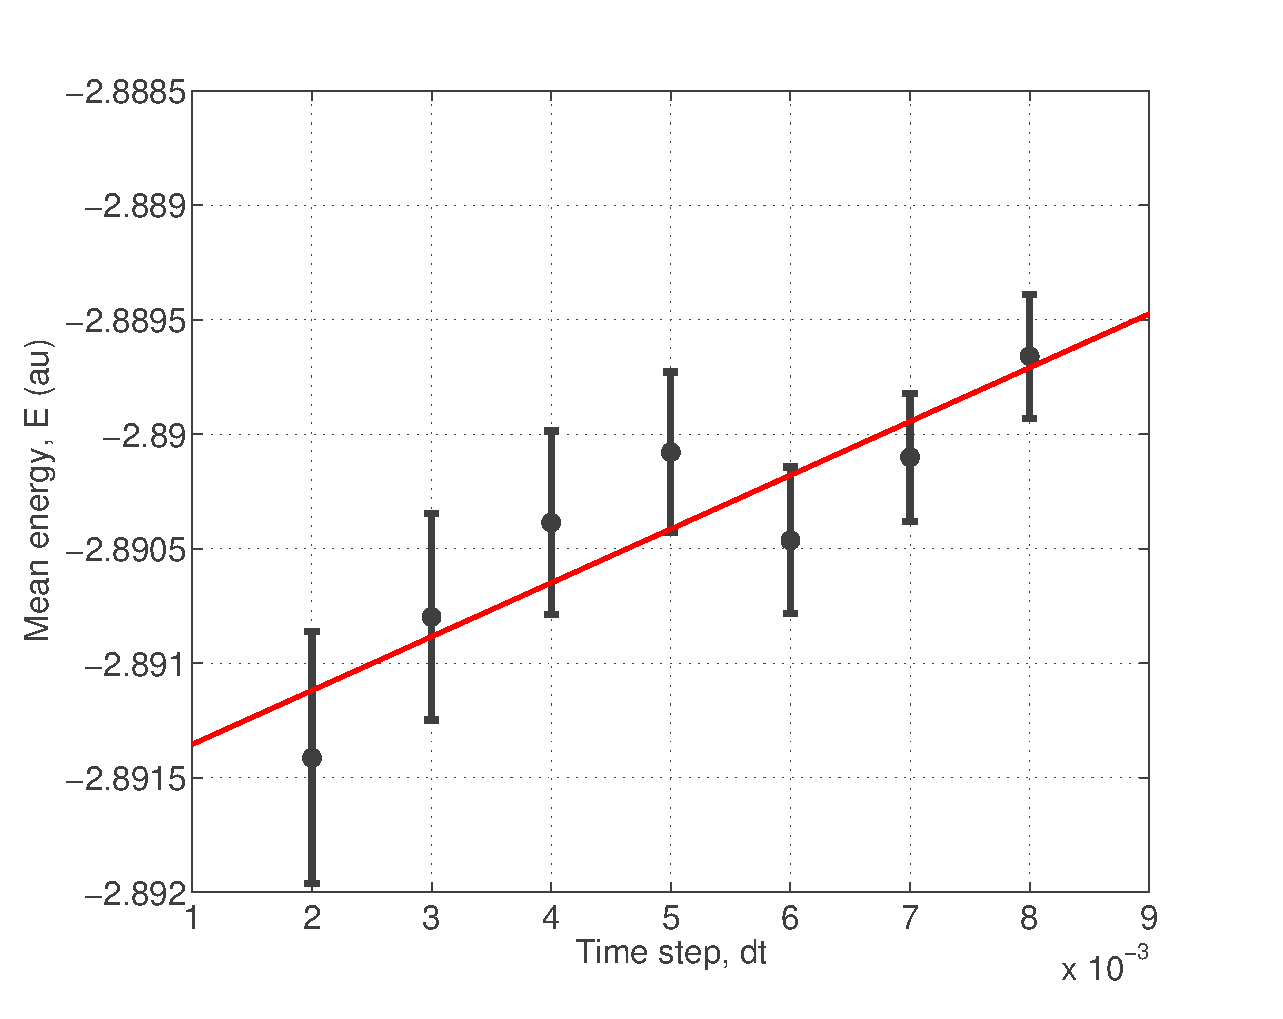
\includegraphics{figures/experimentalData/blocking/blockingDtHe}} &
      \resizebox{50mm}{!}{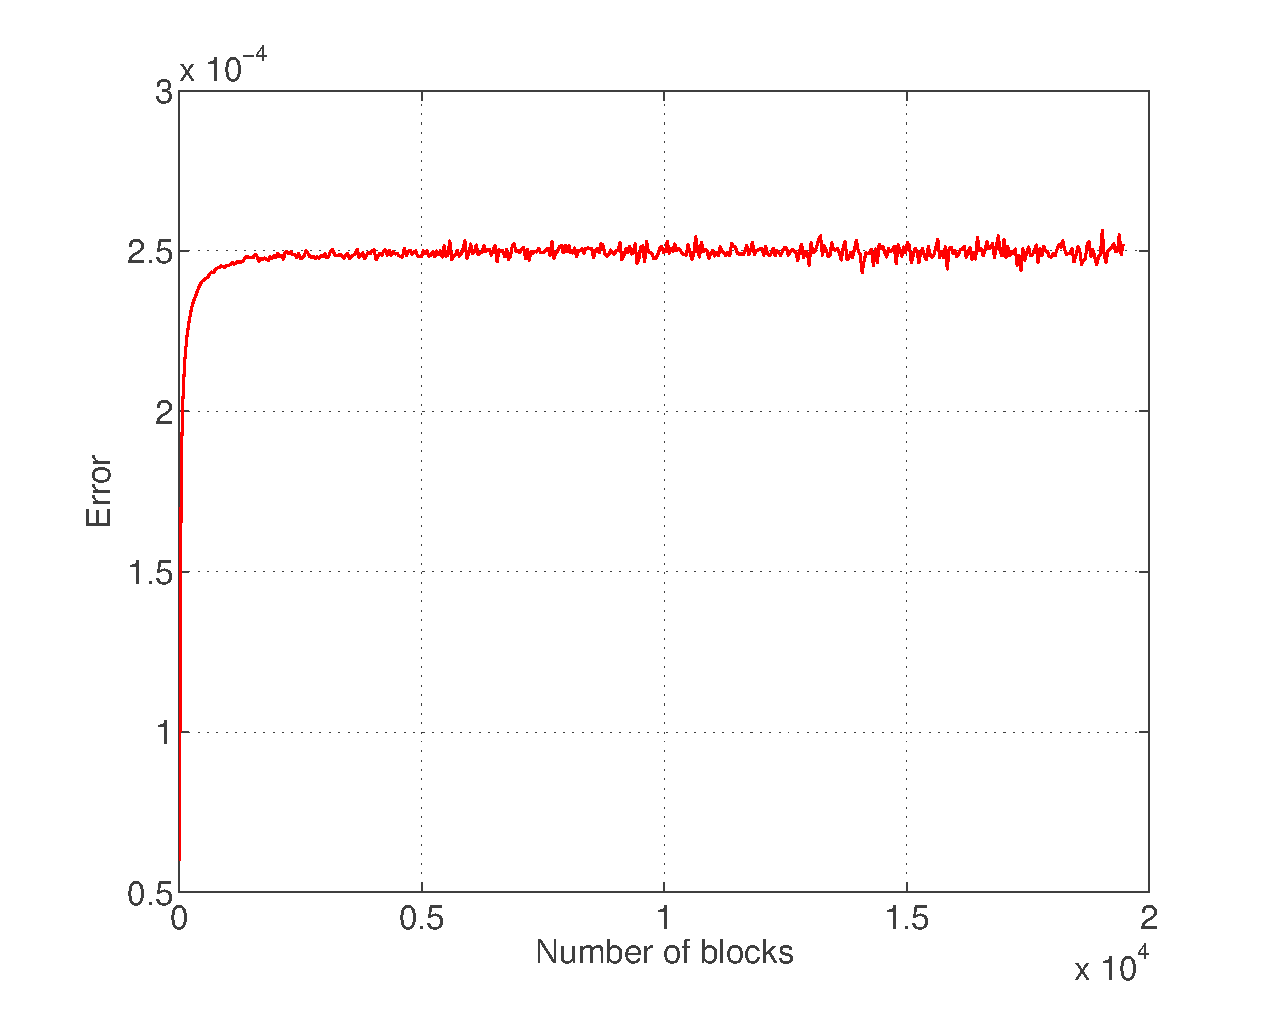
\includegraphics{figures/experimentalData/blocking/blockingHe}} \\
      \end{tabular}
      \caption{To the left we show the  extrapolation to $dt-$zero of the energy for a He atom. To the  right we display the details of the blocking analysis at $dt=0.01$ where the energy $-2.89039 \pm 2.5 \times 10^{-4}\, au$. Experimental setup: $10^7$ Monte Carlo cycles, $10 \%$ equilibration steps with four nodes, with $\alpha = 1.8379$, $\beta = 0.3704$.}
      \label{dtEnergyExtrapolationHe}
    \end{center}
  \end{figure}
  \end{scriptsize}  
\end{frame}




\begin{frame}{Extrapolation of energy to zero dt for Be}
  \begin{scriptsize}
  \begin{table}[!hbt]
  \centering
  \begin{tabular}{cccc}
    \toprule[1pt]
    \textbf{Time step} & \textbf{Energy}, (au)  & \textbf{Error} & \textbf{Accepted moves}, (\%) \\
    \midrule[1pt]
    0.004  &  -14.50321303316  &  1.3e-3  &   99.61\\
    0.005  &  -14.50266236227  &  1.2e-3  &   99.47\\
    0.006  &  -14.50136820967  &  1.1e-3  &   99.32\\
    0.007  &  -14.50314292468  &  1.0e-3  &   99.17\\
    0.008  &  -14.50206184582  &  9.5e-4  &   99.01\\
    0.009  &  -14.50164368104  &  8.5e-4  &   98.85\\
    0.01   &  -14.50145748870  &  8.0e-4  &   98.68\\
    \bottomrule[1pt]
  \end{tabular}\caption{Energy computed for the Be atom and the error associated as a function of the time step. Parameters: $10^7$ Monte Carlo cycles with 10 \% equilibration steps, $\alpha = 3.983$ and $\beta = 0.103$.}\label{blockingDtTableBe}
  \end{table}
  \end{scriptsize}
\end{frame}




\begin{frame}{Extrapolation of energy to zero dt for Be}
  \begin{scriptsize}
  \begin{figure}[!hbt]
    \begin{center}
      \begin{tabular}{cc}
      \resizebox{50mm}{!}{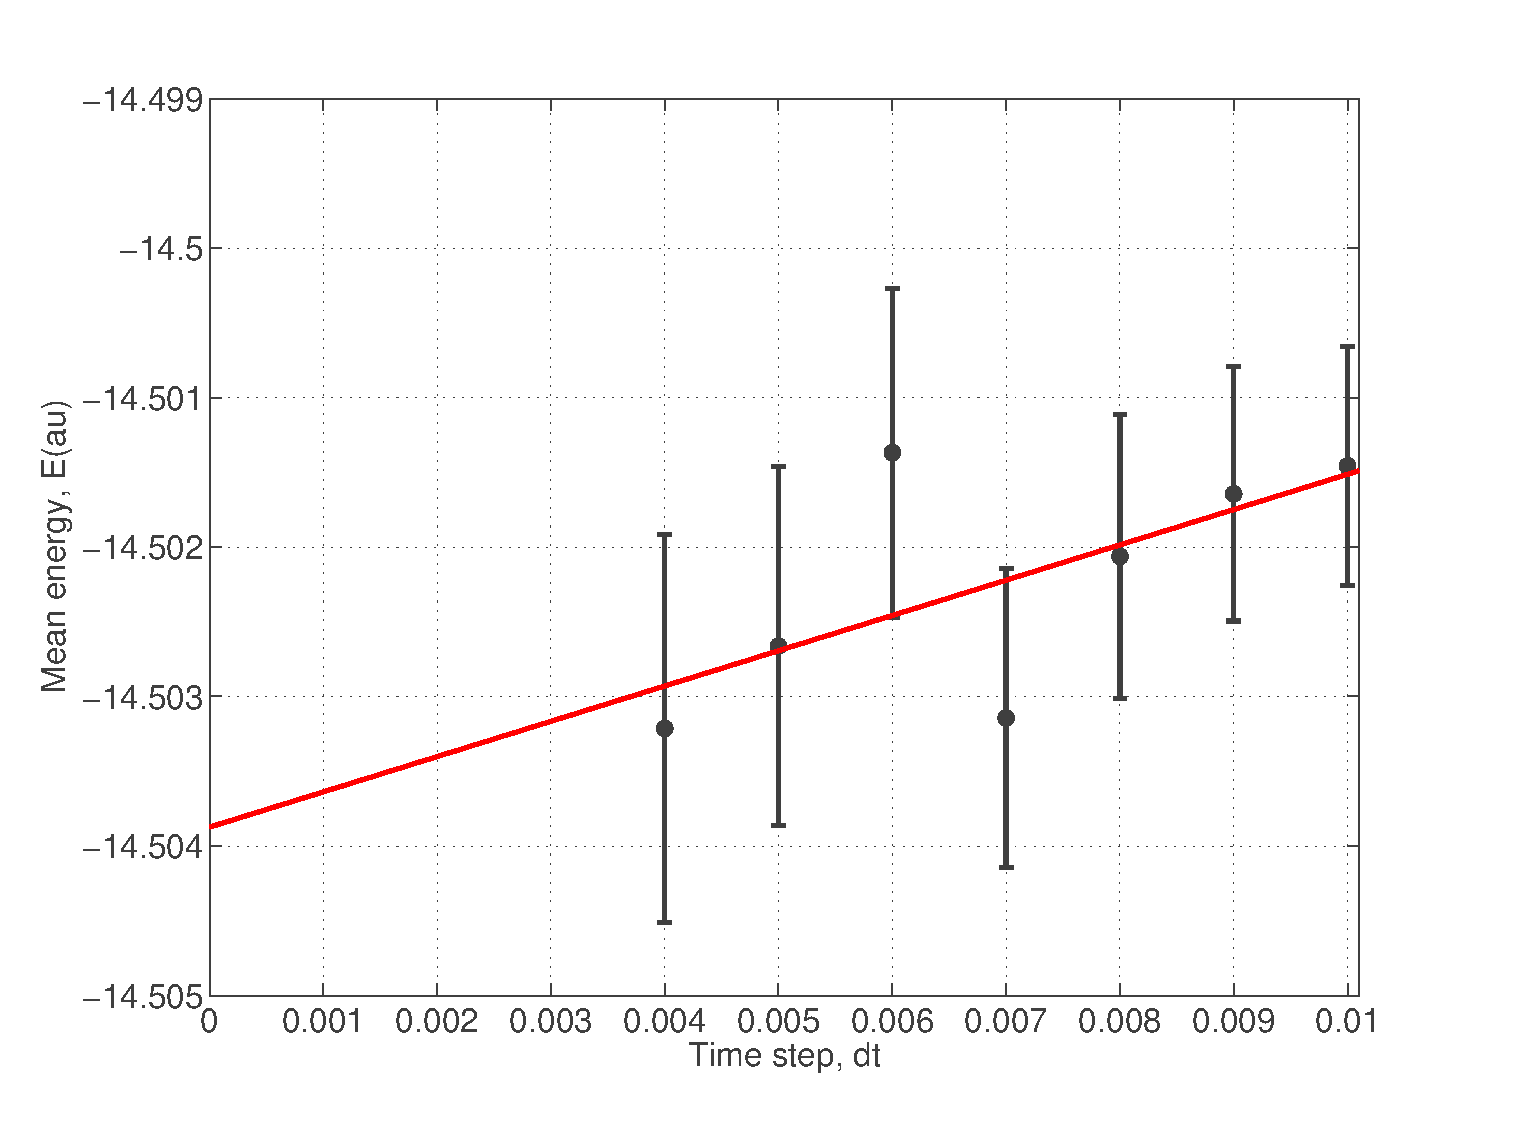
\includegraphics{figures/experimentalData/blocking/blockingDtBe}} &
      \resizebox{50mm}{!}{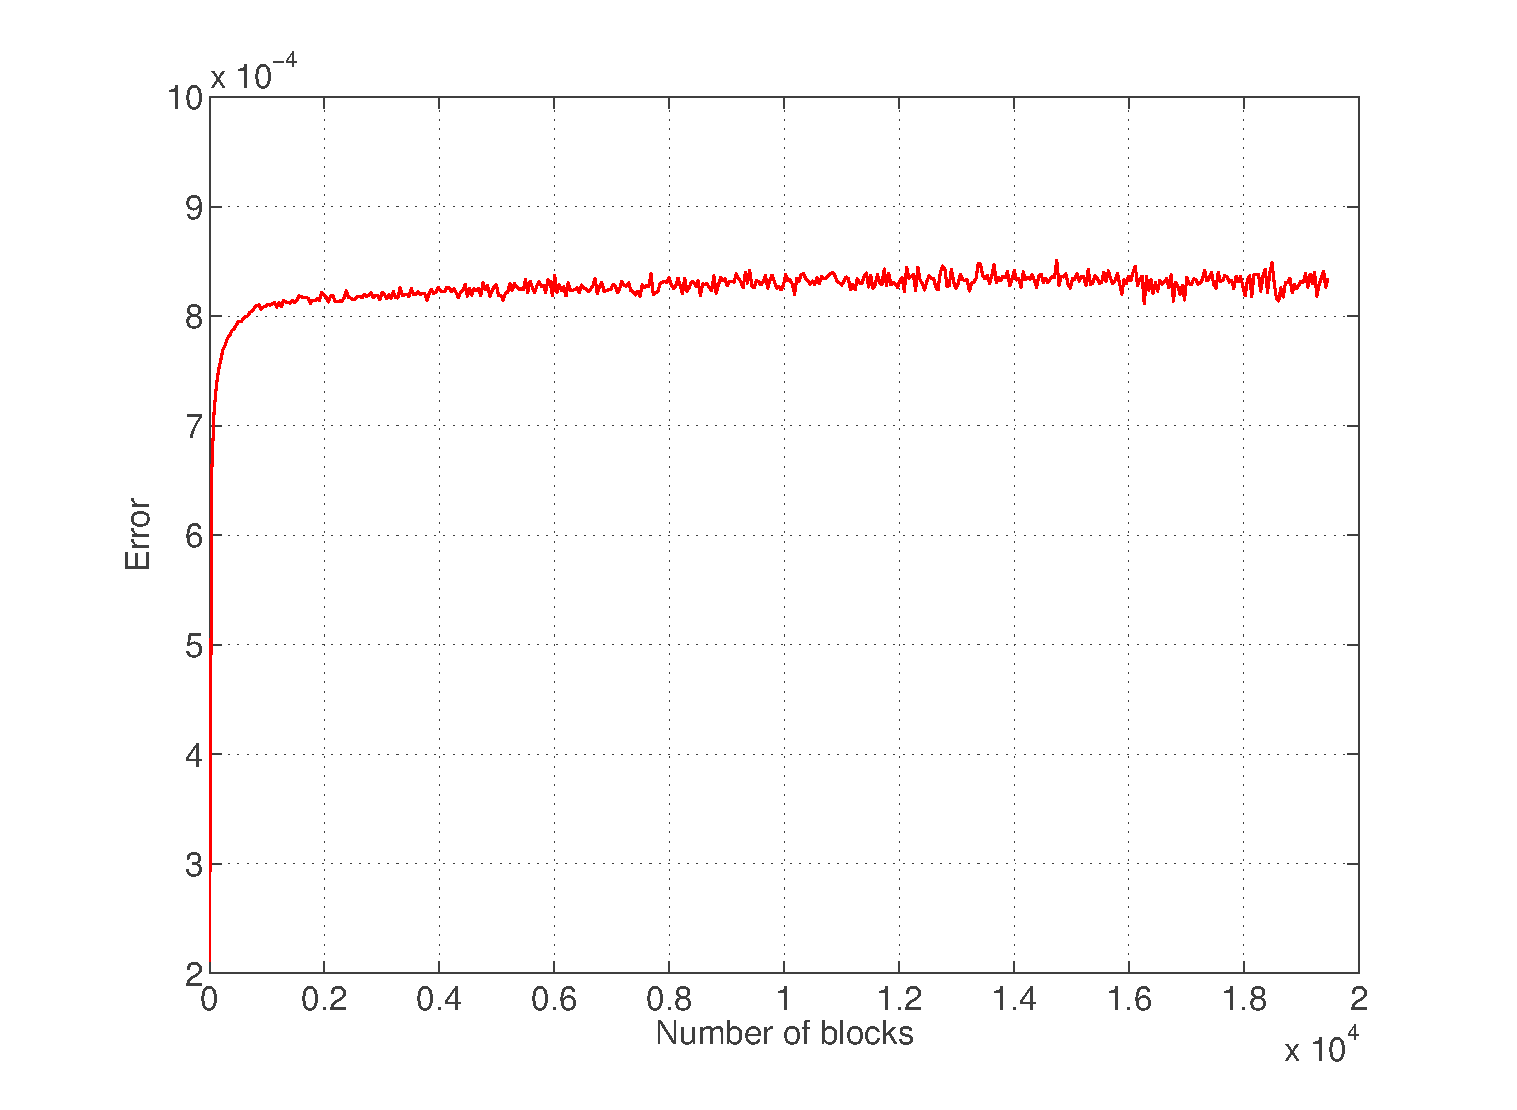
\includegraphics{figures/experimentalData/blocking/plotBlockingBe}} \\
      \end{tabular}
      \caption{Extrapolation to $dt-$zero of the energy (left) and blocking analysis at $dt=0.01$ for the Be atom where the energy $E = -14.50146 \pm 8.5 \times 10^{-4} \, au$. Experimental setup: $10^7$ Monte Carlo cycles, $10 \%$ equilibration steps for four nodes, with $\alpha = 3.983$ and $\beta = 0.103$.}
      \label{dtEnergyExtrapolationBe}
    \end{center}
  \end{figure}
  \end{scriptsize}
\end{frame}



\begin{frame}{Extrapolation of energy to zero dt for 2-$e^-$ electron QD}
  \begin{scriptsize}
  \begin{table}
  \centering
  \begin{tabular}{cccc}
  \toprule[1pt]
    \textbf{Time step} & \textbf{Energy}, (au)  & \textbf{Error} & \textbf{Accepted moves}, (\%) \\
    \midrule[1pt]
    0.01 & 3.000340072477 & 4.5e-5 & 99.95\\
    0.02 & 3.000357900850 & 3.2e-5 & 99.87\\
    0.03 & 3.000364180564 & 2.6e-5 & 99.77\\
    0.04 & 3.000384908560 & 2.2e-5 & 99.65\\
    0.05 & 3.000370330692 & 2.0e-5 & 99.52\\
    0.06 & 3.000380980039 & 1.8e-5 & 99.37\\
    0.07 & 3.000402836533 & 1.7e-5 & 99.21\\
    \bottomrule[1pt]
  \end{tabular}\caption{Results of a blocking analysis for several time steps. The system was a two-dimensional quantum dot with two electrons and $\omega=1.0$. The rest of the parameters were: $10^7$ Monte Carlo cycles with 10 \% equilibration steps, and $\alpha = 0.99044$ and $\beta = 0.39994$ taken from  Albrigtsen(2009).}\label{blockingDtTable2DQDot2e}
  \end{table}
  \end{scriptsize}
\end{frame}




\begin{frame}{Extrapolation of energy to zero dt for 2-$e^-$ electron QD}
  \begin{scriptsize}
  \begin{figure}[!hbt]
    \begin{center}
      \begin{tabular}{cc}
      \resizebox{50mm}{!}{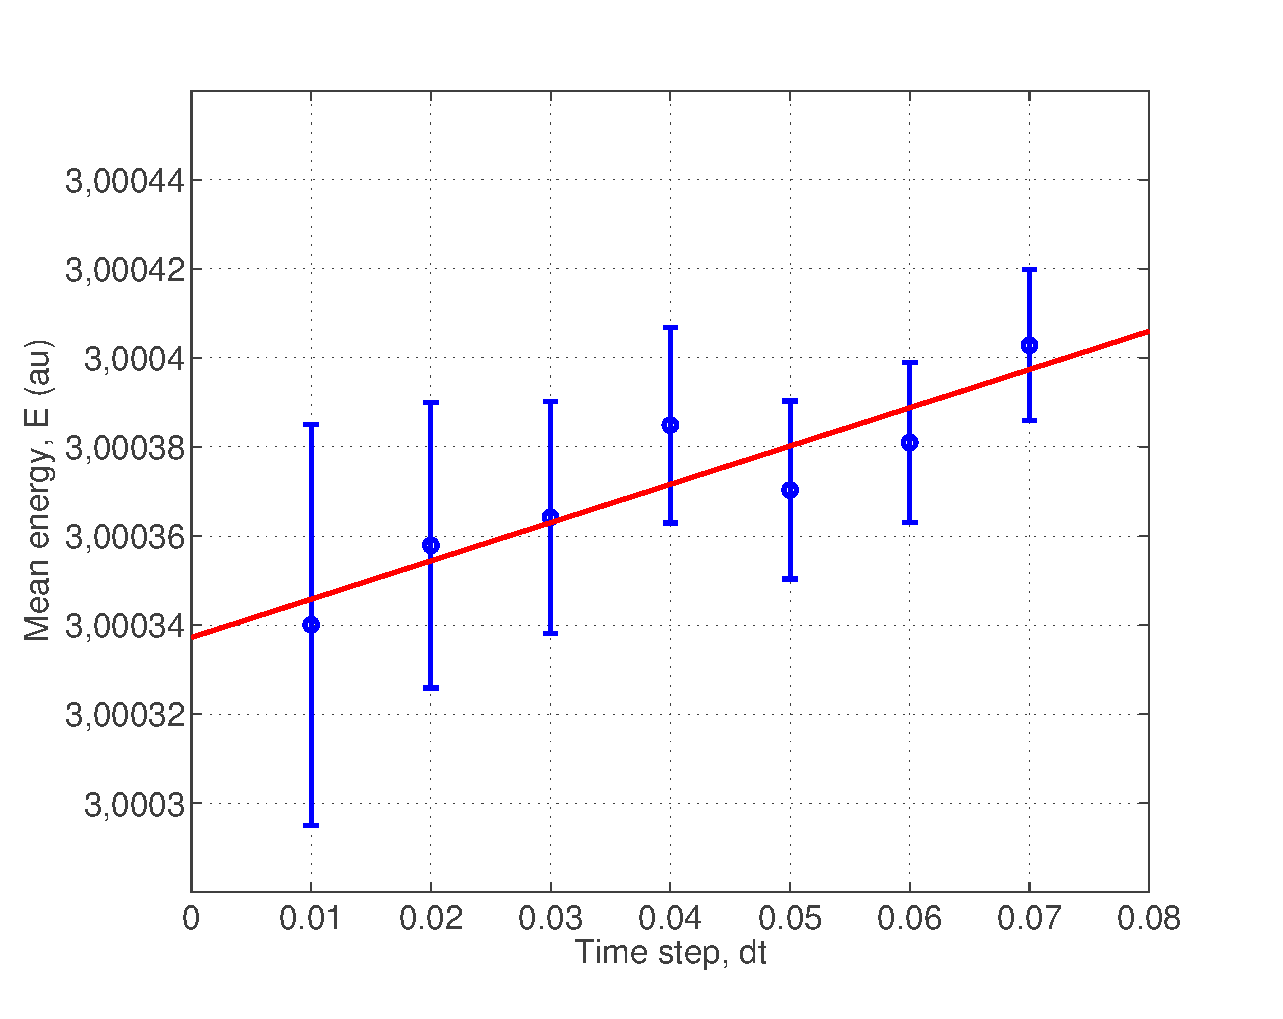
\includegraphics{figures/experimentalData/blocking/dtPlot2DQDot2e}} &
      \resizebox{50mm}{!}{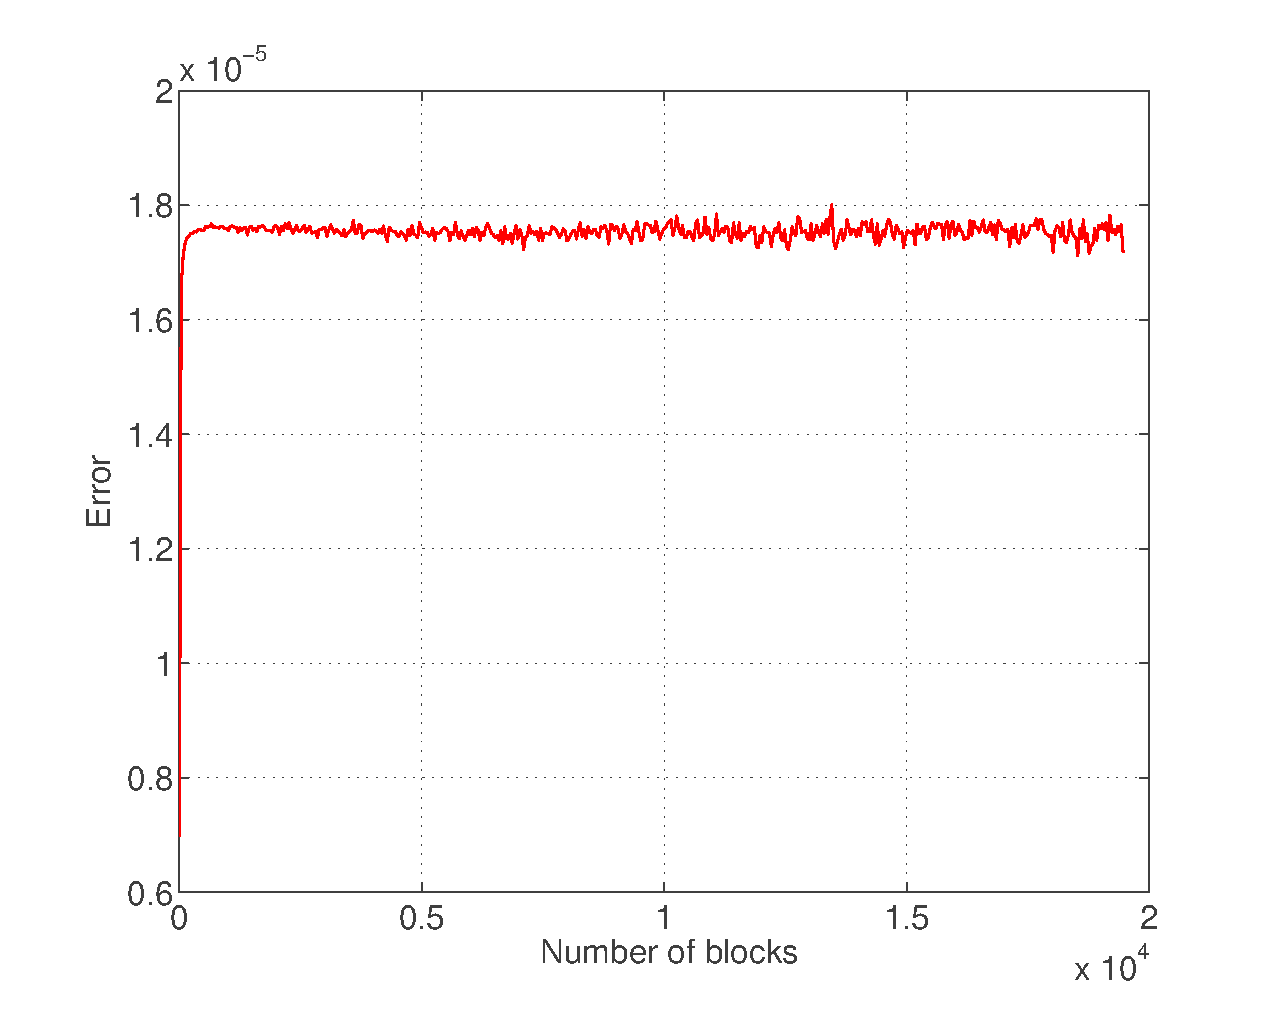
\includegraphics{figures/experimentalData/blocking/block2DQDot2edt0p06}} \\
      \end{tabular}
      \caption{Extrapolation to $dt-$zero of the energy for a two-dimensional quantum dot with two electrons (left) and mean energy error ($E_{min} = 3.000381 \pm 1.8 \times 10^{-5} \, au$) at $dt=0.06$ as a function of the number of blocks for a 2DQDot2e (right). Parameters of simulation: $1 \times 10^7$ Monte Carlo steps with 10 \% equilibration steps, $\alpha = 0.99044$ and $\beta = 0.39994$. The error varies from $1.7 \times 10^{-5}$ at $dt = 0.07$ to $4.5\times 10^{-5}$ at $dt = 0.01$.}
      \label{dtEnergyExtrapolation2DQdot2e}
   \end{center}
  \end{figure}
  \end{scriptsize}
\end{frame}



\begin{frame}{Extrapolation of energy to zero dt for 6-$e^-$ electron QD}
  \begin{scriptsize}
  \begin{table}
  \centering
  \begin{tabular}{cccc}
    \toprule[1pt]
    \textbf{Time step} & \textbf{Energy}, (au)  & \textbf{Error} & \textbf{Accepted moves}, (\%) \\
    \midrule[1pt]
    0.01 & 20.19048030567 & 4.0e-4 & 99.90\\
    0.02 & 20.19059799459 & 2.8e-4 & 99.75\\
    0.03 & 20.19045049792 & 2.4e-4 & 99.55\\
    0.04 & 20.19069748408 & 2.0e-4 & 99.34\\
    0.05 & 20.19066469178 & 1.8e-4 & 99.10\\
    0.06 & 20.19064491561 & 1.7e-4 & 98.85\\
    0.07 & 20.19078449010 & 1.6e-4 & 98.58\\
    \bottomrule[1pt]
  \end{tabular}\caption{Results of a blocking analysis for several time steps. The system was a two-dimensional quantum dot with six electrons and $\omega=1.0$. The rest of the parameters were: $10^7$ Monte Carlo cycles with 10 \% equilibration steps, and $\alpha = 0.926273$ and $\beta = 0.561221$ taken from Albrigtsen (2009).}\label{blockingDtTable2DQDot6e}
  \end{table}
  \end{scriptsize}
\end{frame}




\begin{frame}{Extrapolation of energy to zero dt for 6-$e^-$ electron QD}
  \begin{scriptsize}
  \begin{figure}[!hbt]
    \begin{center}
      \begin{tabular}{cc}
      \resizebox{50mm}{!}{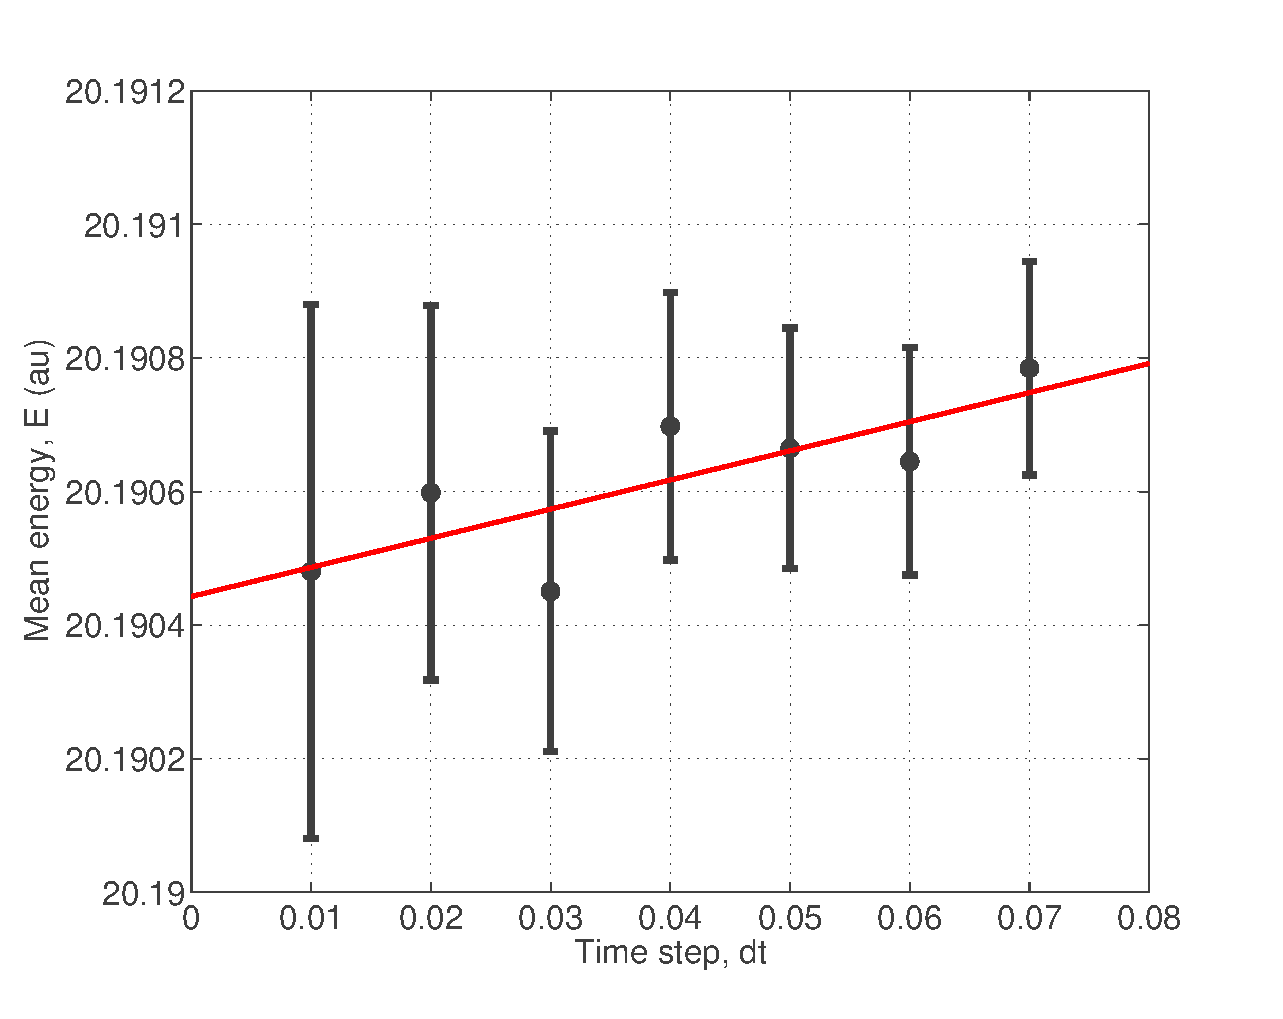
\includegraphics{figures/experimentalData/blocking/plotDtStudy2DQDot6e}} &
      \resizebox{50mm}{!}{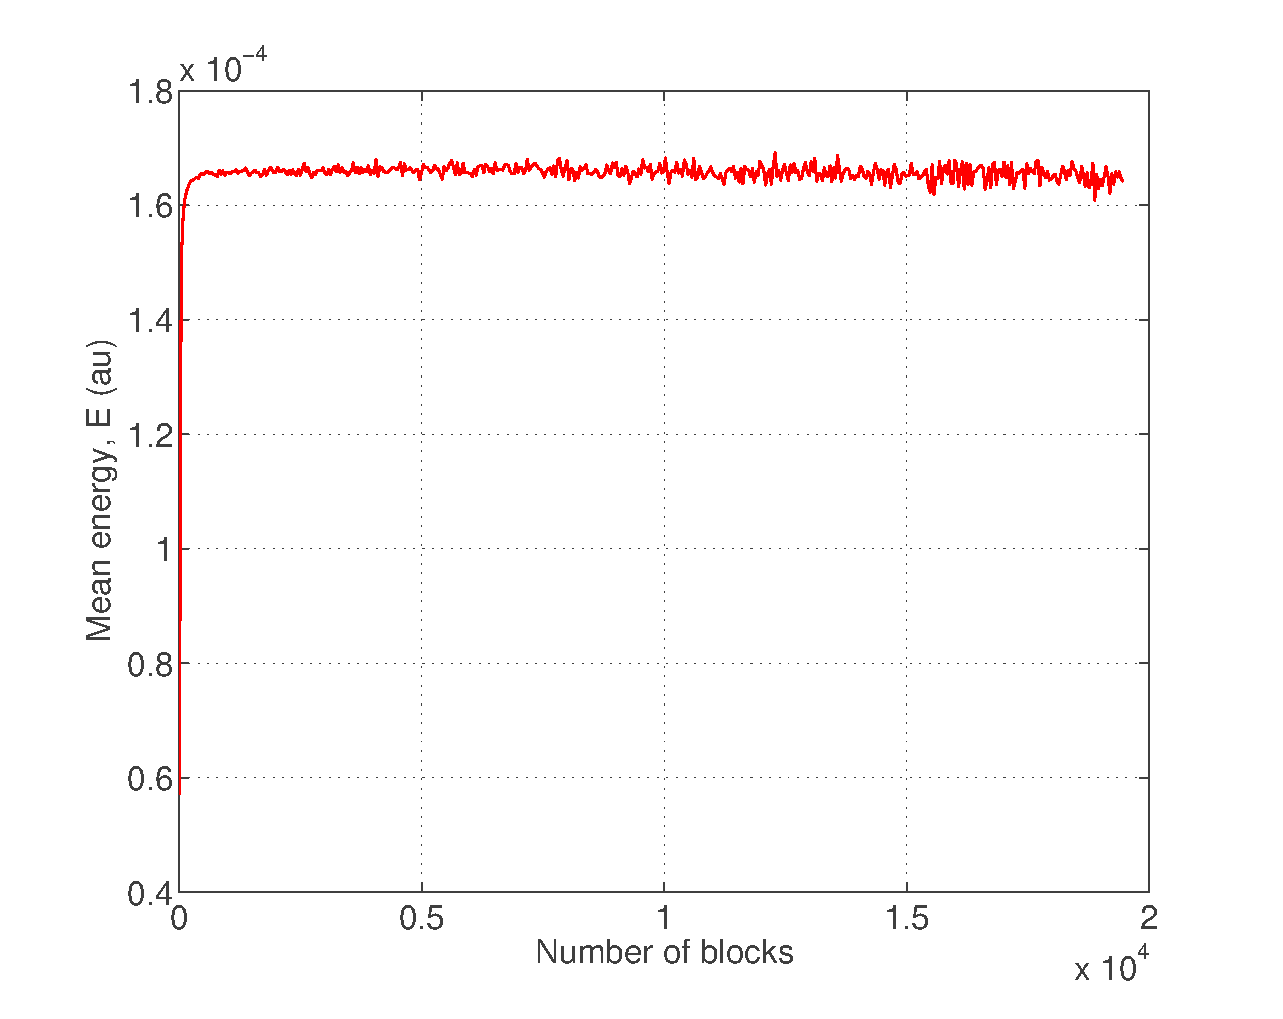
\includegraphics{figures/experimentalData/blocking/blockAnalyse2DQDot6e}}\\
      \end{tabular}
      \caption{Extrapolation to $dt-$zero of the energy for a two-dimensional quantum dot with six electrons (left) and mean energy error ($E_{min} = 20.190645 \pm 1.7 \times 10^{-4} \, au$) at $dt=0.06$ as a function of the number of blocks for a 2DQDot6e (right). Parameters of simulation: $10^7$ Monte Carlo steps with 10 \% equilibration steps, $\alpha = 0.926273$ and $\beta = 0.561221$ running with four nodes.}
      \label{dtEnergyExtrapolation2DQdot6e}
    \end{center}
  \end{figure}
  \end{scriptsize}
\end{frame}




\begin{frame}{Extrapolated energy to zero dt for atoms and QD}
  \begin{scriptsize}
  \begin{table}
  \centering
  \begin{tabular}{lr}
    \toprule[1pt]
    \textbf{System} & \textbf{Energy}, (au)\\
    \midrule[1pt]
    He &  -2.8913\\
    Be &  -14.5039\\
    2DQDot2e & 3.0003\\
    2DQDot6e & 20.1904\\
    \bottomrule[1pt]
  \end{tabular}\caption{Energies estimated using zero-dt extrapolation.%$\omega~=~1.0$ for quantum dots.
  }\label{energyCuts}
  \end{table}
  \end{scriptsize}
\end{frame}



\subsection{Influence of the \# MC cycles}
\begin{frame}{Influence of the \# MC cycles on the statistical error}
  \begin{scriptsize}
  \begin{figure}[!hbt]
    \begin{center}
%        \begin{tabular}{cc}
      \resizebox{55mm}{!}{\includegraphics{figures/experimentalData/errorVsMC/errorVsMonteCarloBe}}
%       \resizebox{55mm}{!}{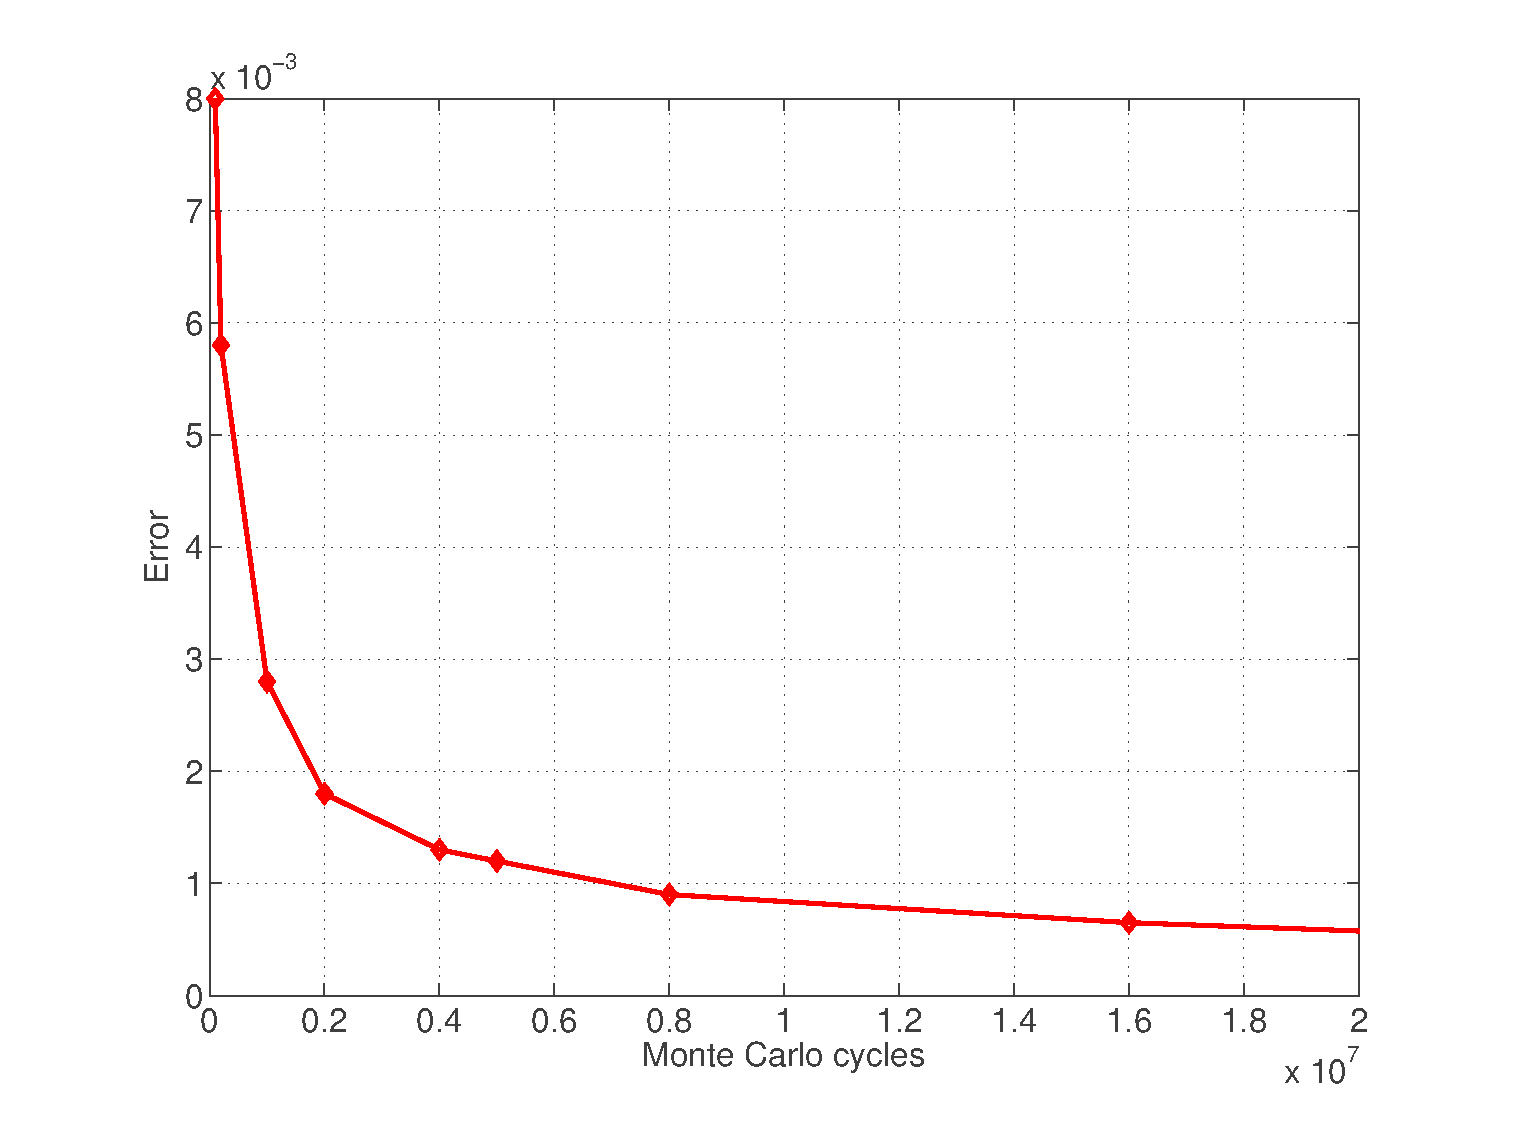
\includegraphics{figures/experimentalData/errorVsMC/errorVsMonteCarloBeZoom}}\\
%        \end{tabular}
      \caption{Error in the energy obtained by blocking for a Be atom as a function of the number of Monte Carlo cycles. The set up for the experiment was: $dt = 0.01$, $\alpha = 3.981$, $\beta = 0.09271$, 10 \% equilibration steps by run in parallel with four processors.}
      \label{errorVsMcBe}
    \end{center}
  \end{figure}
  \end{scriptsize}
\end{frame}











\newpage
\chapter{Discussion}
This study demonstrates the potential of PINNs for efficient simulations of cardiac electrophysiology. The training of PINNs was performed using various geometrical configurations, including 1D and 2D structured geometries, as well as  MRI-based geometries. The main, novel, contributions of this work are as follows:
\begin{itemize}
    \item An MRI-derived Cardiac Electrophysiology PINN model which includes image-informed scar regions with reduced conductivity.
    \item Extension of the PINN model to variable conductivity values, which  removes the need for the PINN to be retrained when simulating scenarios with differing conductivities, as occurs in real-world physiological and pathophysiological scenarios. 
\end{itemize}

\section{1D cable and 2D Square geometry}

The PINNs successfully reproduced the electrical wave propagation in 1D cable and 2D square geometries. The models showed high accuracy in capturing the dynamics.  Specifically, the RMSE values were consistently low across different training sample sizes and noise levels. For both the 1D and 2D scenarios, our results exhibit a strong concordance with the RMSE values reported in \cite{EP-PINNs}, which specified $\mathrm{RMSE}\leq 2.5 \times 10^{-2}$ for the 1D case when using $100$ training and $\mathrm{RMSE}\leq 3.0 \times 10^{-2}$ for the 2D structured grid scenario with $1.4\times 10^5$ training points, without added noise in both cases. If we exclude the outliers seen in Figure \ref{fig:RMSE_1D}, which were models getting stuck early on in training, we get $\mathrm{RMSE\leq 3.6\times10^{-2}}$ in the 1D scenario. In the 2D scenario (Figure \ref{fig:RMSE_2D}), we have $2.0\times10^{-3}\geq\mathrm{RMSE}\leq 1.5 \times 10^{-2}$ when using $10^4$ training points, even with normally distributed noise with a standard deviation of approximately $10\%$ of the maximum $V$ value.
Nevertheless, our models demonstrated significant variability when trained on smaller and noisier datasets (Figures \ref{fig:RMSE_1D} and \ref{fig:RMSE_2D}). Additionally, We conducted a more extensive investigation into the variability of the models compared to \cite{EP-PINNs}, which trained only 5 models, whereas we trained 10 models.
 Furthermore, the authors utilized DeepXDE~\cite{lu2021deepxde}, a library designed for Physics-Informed machine learning and employed a different optimization process consisting of first training on the data only with Adam for a few epochs, followed by training using the complete loss and finally finishing training with the L-BFGS optimization algorithm~\cite{L-BFGS}. Therefore, variations in both implementation and training procedures could have contributed to these observed differences.
The presence of extreme outlier in Figures \ref{fig:RMSE_1D} and \ref{fig:RMSE_2D},  can likely be attributed to the inherent stochastic nature of neural network training. Specifically, from the random initialization of the neural network parameters.
%In the  models also converged much faster, possibly due to the absence of input scaling in their approach, which may have led to the saturation of activation functions, resulting in very small gradients and consequently slow learning. However, to confirm this hypothesis, an examination of the gradients during training would be required.
%-Different implementation DeepXDE vs PyTorch
%-Our models did converge much faster: I think it's because they didn't scale the inputs, which means the activation function is getting saturated->gradients very small-> very slow learning.
%EP-PINNs 1D RMSE ≤ 2.5 × 10−2 . 2D RMSE < 3.0 × 10−2
%For both 1D and 2D scenarios, our findings align closely with the RMSE values documented in \\cite{EP-PINNs}, which indicated $\mathrm{RMSE}\leq 2.5 \times 10^{-2}$ for the 1D case and $\mathrm{RMSE}\leq 3.0 \times 10^{-2}$ for the 2D case.  Our models showed high variability when trained with smaller and noisy sample sizes(Figures \ref{fig:RMSE_1D} and \ref{fig:RMSE_2D}). We prune the variability of the models a bit more than EP-PINNs than only trained 5 models insted of 10 like we did.
%The outlier cases in Figure\ref{fig:box_plot_MRI} failed to converge which shows PINNs sensitivity to initialization.


\section{MRI-based 2D geometry with isotropic conductivities}
Extending the analysis to more anatomically accurate models, the novel isotropic MRI-based 2D geometry experiments further highlight the strengths of PINNs. The comparison between FEM and PINN results, particularly the relative $ L_1$ error values of 0.02 at both the 100 ms and 530 ms time points demonstrates the effectiveness of PINNs in handling complex geometrical structures derived from MRI data. In particular, this experiment shows that PINNs can reproduce the dynamics of electrophysiological wave propagation from sparse measurements ($100$ spatial points) and noisy measurements ($\sigma=8.0$), which is crucial in a clinical setting where data are often limited. Although this is a proof-of-concept and further refinement is needed, it provides a promising foundation for future clinical applications, supporting Hypothesis 2 by showing improved computational efficiency and maintaining accuracy in simulating these complex dynamics. 
In contrast to the work by Xie and Yao \cite{PDL}, which utilized a 3D geometry with a relatively sparse $1094$ vertices, our 2D model employed $72434$ vertices and achieved an \(RL^2\) error of $0.05$ compared to their \(RL^2\) error of $0.08$. Although these results are not directly comparable due to the dimensional difference, our initial experiments (structured geometries) suggest that there isn't significant loss in accuracy when transitioning from 1D to 2D with our approach. Therefore, similar accuracy could be maintained when extending our work from 2D to 3D.
This comparison is particularly relevant as prior work in this field is scarce, and Xie and Yao \cite{PDL} provide an example of an isotropic model in a 3D geometry, demonstrating that accurate PINN solutions are possible in such complex structures. However, it is important to note that the 3D study did not cover the modeling of scars nor MRI-derived geometries, which are unique contributions of our work. 
%number of collocation points is a limiting factor(memory usage).

%Scaling inputs (-2,2) was better than both standardization (mean 0 and unit variance) and scaling(-1,1). 


\section{MRI-based 2D geometry with anisotropic conductivities}
The anisotropic MRI-based 2D geometry experiment demonstrates the generalization capabilities of PINNs.
Figures \ref{fig:box_plot_MRI_aniso} and \ref{fig:RL1_anisotropic} reveal several noteworthy patterns. Contrary to initial expectations, there is no marked distinction in the relative $L^1$ error between training, interpolation, and extrapolation datasets. This could be attributed to the majority of the training dataset being unseen by the model, resulting in similar performance across different subsets. Additionally, there appears to be a slight increase in error with higher conductivity values. This trend could be explained by the fact that larger conductivity corresponds to faster wave speeds, which makes the model more susceptible to errors due to slight phase shifts. 
 %The relative \( L_1 \) error comparison for interpolating and extrapolating conductivities (Figure \ref{fig:RL1_anisotropic}) reveals a slight increase in error during extrapolation, yet it remains comparable to the training data error during interpolation. This indicates that while the model performs exceptionally well within the range of the training data, its accuracy slightly diminishes when predicting beyond this range. However, the error increase is not substantial, demonstrating the robustness of PINNs in handling varying conductivity scenarios.
 
This novel approach, unprecedented in the context of cardiac electrophysiology, is particularly noteworthy as it illustrates the possibility to create a neural network based solver capable of running different simulations in a fraction of a second by simply inputting different conductivities. In contrast, the FEM method necessitates a full repetition of the process for every new simulation. Additionally, the results show that the wave propagation slows down in regions of low conductivity, indicating that the PINN has successfully learned how conductivity affects wave propagation. These findings support Hypotheses 1 and 3, and underscore the significant advantages of using PINNs over traditional methods in terms of both speed and adaptability. 
The PINN training process can be slow and resource-intensive, presenting a significant investment in computational resources and time. However, our study demonstrates that this investment can be highly beneficial. Once trained, our PINN model can efficiently handle varying conductivities as inputs, offering significant flexibility, adaptability and fast inference times.
%Discuss inference times and training time: PINNs are expensive(GPUs and need a lot of memory) and slow to train, but we show that this investement can be worth it because our model can handle varying conductivities as inputs and inference time is very short and inexpensive.

%This novel approach, unprecedented in the context of cardiac electrophysiology provides a promising avenue 
\newpage
In this chapter, we have developed three many-body methods we will use throughout this thesis. The most fundamental of these methods is the Hartree-Fock theory, which will recover a reasonable amount of the system's energy. It is an independent particle model, so it cannot account for the energy from interacting particles. The first post-Hartree-Fock method we developed, so-called because it improves the Hartree-Fock result, was many-body perturbation theory (MBPT) which provides a convenient truncation scheme that allows for systematic improvements to the Hartree-Fock results. The final many-body method, developed in great detail due to its importance later in this thesis, was coupled cluster theory, which is more accurate than MBPT but much more time-consuming. Coupled cluster theory also provides a convenient truncation scheme and, at the triple level, allows us to recover most of the system's energy even with the method being truncated. Now that we have developed our many-body methods, the next chapter will be devoted to developing the system to which these methods will be applied: infinite matter.
\appendix
\documentclass[../../master.tex]{subfiles}

\begin{document}

\chapter{Natural units: Hartree atomic units \label{units}}
\newcommand{\M}{\mathrm{M}}
\renewcommand{\L}{\mathrm{L}}
\newcommand{\T}{\mathrm{T}}
\renewcommand{\C}{\mathrm{C}}
When working within a specific branch of physics, it is often useful to deviate from the every-day SI units of measurements and instead use units which are \emph{natural} to the systems under study. Since we are working with "small" systems, the SI \emph{meter}, \emph{second}, \emph{kilogram}, and \emph{coulomb} are of little use to us. Instead we will work in a system of units in which we define the mass of the electron, $m_e$, to be the scale by which we measure all other masses. This obviously means the numerical value of the electron mass becomes unity, $m_e=1$. In the same way, we will use Planck's constant, $\hbar$, as the scale by which we measure angular momentum and action, the electron charge, $e$, will be our scale for electrical charge, and finally Coulomb's constant, $k_e$, will be our scale of electric permittivity. 

The usual way to state this is to set $\hbar=e=m_e=k_e=1$, and the system of units derived from these four definitions is called Hartree atomic units. We can think of this as the \emph{natural} system of units for the Hydrogen atom system. To better see why this is the case, let us combine these four quantities in such a way as to produce a length. 

In terms of the four fundamental dimensions of physics: Length(L), time(T), mass(M), and charge(C), the units of $\hbar$, $m_e$, $e$, and $k_e$ are $\left[\hbar\right]=\mathrm{M}\mathrm{L}^2\mathrm{T}^{-1}$, $\left[m_e\right]=\mathrm{M}$, $\left[e\right]=\mathrm{C}$, and $\left[k_e\right]=\mathrm{M}\mathrm{L}^3\mathrm{C}^{-2}\mathrm{T}^{-2}$, respectively. Combining arbitrary powers of these four constants gives 
\begin{align}
\left[\lambda(a,b,c,d)\right] &= \left[k_e^a \hbar^b m_e^c e^d\right] =  \left(\M^a \L^{3a} \C^{-2a} \T^{-2a} \right) \left(\M^b \L^{2b} \T^{-b} \right) \left( \M^c \right) \left( \C^d \right) \nn\\
%%
&= \L^{2a+3b} \T^{-a-2b} \M^{a+b+c} \C^{-2b+d}.
\end{align}
There is exactly one way to realize a length from these exponents, i.e. solving the four equations $2a+3b=1$, $-a-2b=0$, $a+b+c=0$, and $-2b+d=0$: $a=-1$, $b=2$, $c=-1$, and $d=-2$. This means that the natural length scale of our problem is simply (up to a numerical constant)
\begin{align}
\L_\text{scale} &= a_0 = k_e^{-1} \hbar^{2} m_e^{-1} e^{-2} = \frac{\hbar^2}{k_e m_e e^2} = \frac{ 4\pi \varepsilon_0 \hbar^2 }{m_e e^2},
\end{align}
which re recognize as simply the \emph{Bohr radius}. 

We can go through this same exercise to find a natural \emph{time} scale for our system. There is a unique way to combine the exponents $a$, $b$, $c$, and $d$ in order to realize a time, namely $a=-2$, $b=3$, $c=-1$, $d=-4$, or
\begin{align}
\T_\text{scale} &= k_e^{-2} \hbar^3 m_e^{-1} e^{-4} = \frac{\hbar^3 }{k_e^2 m_e e^4} = \frac{\hbar a_0}{k_e e^2}.
\end{align}
This is the revolution time of an electron in the lowest lying hydrogen state in the Bohr model (apart from a factor of $2\pi$).

From $a_0$ and $\T_\text{scale}$ we can find the natural energy scale,
\begin{align}
\mathrm{E}_\text{scale} &= m_e \frac{a_0^2}{a_0^2 \left(\frac{\hbar}{k_e e^2}\right)^2} = \frac{m_e k_e^2 e^4}{\hbar^2} \equiv E_h,
\end{align}
which we will call a Hartree. 

Finally, before we go on we may use the expression for the \emph{fine structure constant} to find the numerical value of $c$ in this system. From 
\begin{align}
\alpha &= \frac{k_e e^2}{\hbar c} \Rightarrow c = \frac{k_e e^2}{\hbar \alpha} = \frac{1}{\alpha} \simeq 137,
\end{align}
after substituting $\hbar=e=k_e=1$.













\chapter{Basics of numerical integration\label{numericalintegration}}
\subsection*{Riemann integral and Riemann integrable functions}
Given a function $f(x)$ and a closed finite subset of $\mathbb{R}$, $[a,b]$ with $a<b$, a \emph{Riemann sum} of $f$ is defined as the sum of values attained on $n$ sub-intervals of $[a,b]$, i.e.
\begin{align}
S_n = \sum_{i=1}^n (x_i-x_{i-1}) \, f_i.
\end{align}
The $x_i$s here define the partitionining into sub-intervals $[x_{i-1},x_i]$ (i.e. $a=x_0<x_1<\dots< x_{n-1}<x_n=b$), while $f_i\equiv f(\xi_i)$ with $\xi_i$ \emph{some} point in sub-interval $i$. 

A sufficient condition for the \emph{Riemann integral} to exist for the function $f$ is that \emph{any} such sum (any choice of $x_i$ [for which $\max_{i}|x_i-x_{i-1}|\rightarrow0$] and $\xi_i$) converge to the same value in the limit $n\rightarrow \infty$ \cite{davis}\comment{p7}. In this case we say
\begin{align}
\lim_{n\rightarrow \infty} S_n = S = \int_a^b f(x)\dx,
\end{align} 
and that $f$ is Riemann integrable.

A less strict, but still sufficient condition is to chose $\overline{f_i}=\max\{f(x):x\in[x_{i-1},x_i]\}$ and $\underline{f_i}=\min\{f(x):x\in[x_{i-1},x_i]\}$ and then only demand that the two sums converge to a common limit \cite{lindstrom}\comment{p366}, 
\begin{align}
\mat{rcccl}{
\displaystyle\lim_{n\rightarrow \infty}\overline{S_n} & = & \displaystyle\lim_{n\rightarrow \infty}\sum_{i=1}^n (x_i-x_{i-1})\overline{f_i} \\
% 
\\[-1em] 
%
& = & \displaystyle\lim_{n\rightarrow \infty}\sum_{i=1}^n (x_i-x_{i-1})\underline{f_i} & = & \displaystyle\lim_{n\rightarrow \infty}\underline{S_n} \\
%
\\[-1.5em] 
% 
&&&=& \displaystyle \int_a^bf(x)\dx.
}\nn
\end{align}

Although easier than checking \emph{every possible} Riemann sum, checking that the two upper and lower sums converge to a common limit is still a somewhat tedious procedure for checking integrability. In fact it turns out that a sufficient condition on $f$ is that it is continuous and bounded on $[a,b]$ \cite{davis}\comment{p7}. The latter condition is not necessary on a finite interval since all continuous functions on a closed finite domain are bounded according to the extreme value theorem. However, if we extend the limits of integration to an infinite interval, for example $[0,\infty)$, then the boundedness of $f$ is not guaranteed by the continuity we need to explicitly demand $|f(x)|<\infty$ for all $x\in[a,b]$.

It is easy to see that the converse is \emph{not} true. Any Riemann integrable function is not automatically continuous. Take for example the integral over $[0,1]$ with the step function 
\begin{align}
f(x) = \left\{\mat{lcr}{1 & \text{if} & x>1/2 \\ 0 & \text{else} }\right..
\end{align}
Even though the upper and lower Riemann sums both attain the value $1/2$ in the limit $n\rightarrow \infty$ and the function is Riemann integrable, it demonstrably is not continuous. A more careful analysis shows that a less strict but sufficient condition on $f$ is that it be continuous \emph{almost everywhere} on $[a,b]$ (i.e. continuous on all of the interval, except possibly on a subset $C\subset[a,b]$ with measure zero) \cite{mcdonald}\comment{p72}. With this condition, the converse also holds.

\subsection*{Newton-Cotes quadrature}
Since the Riemann integral is defined in terms of the limit of a sum, numerical approximations to it arise naturally from any scheme for choosing $\xi_i$ and the partitioning. One of the simplest possible approximations is to take the midpoint value of each sub-interval to be $\xi_i$ with a uniform mesh of equispaced $x_i$s. This constitutes the {\bf midpoint rule} \cite{davis}\comment{p52}, 
\begin{align}
I\approx \sum_{i=1}^n f(x_{i-1}+\Delta x/2)(x_{i}-x_{i-1})=\Delta x\sum_{i=1}^n f(x_{i-1}+\Delta x/2),
\end{align}
where $\Delta x\equiv (x_i-x_{i-1})$ which is the same for all $i$.

Instead of the midpoint, we can use the \emph{average} of the left and right endpoints of the subinterval as $f_i$. Geometrically, this means we are approximating the integral of each sub-interval by the integral over a right trapezoid with base points at $(x_{i-1},0)$ and $(x_i,0)$ and upper point at the function values $(x_{i-1},f(x_{i-1}))$ and $(x_{i},f(x_{i}))$. The resulting approximation is known as the {\bf trapezoidal rule} \cite{hjorthjensen}\comment{p113},
\begin{align}
I\approx \sum_{i=1}^n \frac{f(x_{i-1})+f(x_{i})}{2}(x_i-x_{i-1}) = \Delta x \sum_{i=1}^n \frac{f(x_{i-1})+f(x_{i})}{2}.
\end{align}

Yet another numerical scheme arises from replacing the integrand in each sub-interval with an interpolating polynomial of degree two, which by construction coincides with $f$ at the endpoints and the midpoint. This constitutes {\bf Simpson's rule} \cite{davis}\comment{p57},
\begin{align}
I&\approx \sum_{i=1}^n (x_i-x_{i-1})\left(\frac{f(x_{i-1}}{6}+\frac{4f(x_{i-1}+\Delta x/2)}{6}+\frac{f(x_{i}}{6}\right) \nn\\
&= \frac{\Delta x}{6}\sum_{i=1}^n \Big( f(x_{i-1}) + 4f(x_{i-1}+\Delta x/2) + f(x_i) \Big).
\end{align}

All three approximations are examples of Newton-Cotes quadrature rules, which approximate the integral by replacing the integrand by interpolating polynomials of order $k$ on each of the $n$ sub-intervals. We can build arbitrarily high order methods by constructing higher order interpolating polynomials within each interval. The interpolation procedure is described for example in \cite{morken}. We have just seen Newton-Cotes method for orders zero (midpoint rule, zero order polynomial [constant]), one (trapezoidal rule, linear polynomial), and two (Simpson's rule, quadratic polynomial). The next few commonly used methods are the third order \emph{Simpson's 3/8 rule} and the fourth order \emph{Boole's rule}.

\subsection*{Gaussian quadrature}
Note that so far we have assumed the sub-intervals to all be the same size. If we drop this requirement, we can construct more advanced rules which exploit some convenient properties of orthogonal polynomials. Gaussian quadrature rules are a set of schemes for numerical intergration in which we extract a \emph{weight function} from the integrand
\begin{align}
\int_a^bf(x)\dx = \int_a^b W(x)g(x)\dx \approx \sum_{i=1}^n w_ig(x_i).
\end{align}
The weight function is associated with a set of orthogonal polynomials, and the integration points $x_i$ are chosen as the zeros of the polynomial of degree $n-1$. Note carefully that $w_i\not=W(x_i)$. The weights $w_i$ can in general be expressed as \cite{krylov}
\begin{align}
w_i=\left(\frac{a_n}{a_{n-1}}\right)\frac{\int_a^b W(x) p_{n-1}(x)^2\dx}{p'_n(x_i)p_{n-1}(x_i)}
\end{align} 
where $p_n(x)$ is the orthogonal polynomial of degree $n$ and $a_n$ is the coefficient of the $x^n$ term in $p_n(x)$. In some cases, the weight function is present in the original integral and the extraction constitutes a strict simplification of the function. For example, with 
Chebyshev polynomials\footnote{The Chebyshev polynomials are solutions to the differential equation 
\begin{align}
(1-x^2)\pder{^2y(x)}{x^2}-x\pder{y(x)}{x} + n^2y(x)=0,
\end{align}
with $n$ a non-negative integer. In general, the solution can be written as \cite{rottmann}\comment{p95} \begin{align}
T_n(x)=\sum_{k=0}^{\lfloor 1/2 \rfloor}{n \choose 2k}(x^2-1)x^{n-2k}.
\end{align}} the weight function takes the form $W(x)=1/\sqrt{1-x^2}$, so trying to apply Gauss-Chebyshev quadrature to the integrand $(x^{10}+x+2)/\sqrt{1-x^2}$ would yield simply $g(x)=x^{10}+x+2$ and we would just have to evaluate $g_i$ according to the zeroes of the $n$th Chebyshev polynomial. Each class of polynomials is associated with a specific interval of integration. For Chebyshev, this is $[-1,1]$. So using our previous example, we note that with only $3!$ integration points (exclamation point for emphasis \emph{and} factorial function) we integrate \emph{exactly}
\begin{align}
I\equiv \int_{-1}^1 \underbrace{\frac{x^{10}+x+2}{\sqrt{1-x^2}}}_{\equiv f(x)}\dx = \sum_{i=1}^6w_i \underbrace{(x^{10}+x+2)}_{g(x)} = \frac{575\pi}{256}.
\end{align}

In general, if $g(x)$ is a polynomial of degree $2n-1$ for a weight function associated with some class of orthogonal polynomials, then the gaussian quadrature rule associated with the same class of polynomials will integrate the original $f(x)$ (recall that $g(x)=f(x)/W(x)$) \emph{exactly} with only $n$ integration points \cite{hjorthjensen}\comment{p119}. 

\subsection*{Multiple integrals}
Both of the aforementioned  rules are straight forward to extend to higher dimensional integrals. For the Newton-Cotes rules, we can simply apply the rule again to the sum resulting from the application of the rule, i.e.
\begin{align}
I_{\text{2D}} &= \int_a^b \int_a^b f(x,y)\,\mathrm{d}x\,\mathrm{d}y \approx \int_a^b\sum_{i=1}^n \Delta x f(\xi_i,y) \,\mathrm{d}y \nn\\
&\approx \sum_{i=1}^n\sum_{j=1}^n \Delta x\Delta y f(\xi_i,\zeta_j).
\end{align}
Since function evaluations on the endpoints of sub-intervals (sub-areas to be precise) coincide with the endpoints of the neighbouring sub-intervals, a number of points may be evaluated multiple times and thus have a higher \emph{weight} in the final sum. For example, the 1D trapezoidal rule carries weights 
\begin{align}
\mat{ccccccccc}{\nicefrac{1}{2} & 1 & 1 & 1 & \dots & 1 & 1 & 1 & \nicefrac{1}{2}},
\end{align}
since 
\begin{align}
\frac{\Delta x}{2}\sum_{i=1}^n\Big(f(x_{i-1}+f(x_i)\Big) &= \frac{\Delta x}{2}\left[f(x_0) + 2\sum_{i=1}^{n-1}\Big(f(x_i)+f(x_{i+1})\Big)\right] \nn\\
&= \frac{\Delta x}{2}\left[f(x_0) + 2\left(\sum_{i=1}^{n-1}f(x_i)\right)+f(x_{n})\right] \nn\\
&= \frac{\Delta x}{2}\left[f(x_0) + 2f(x_1) + 2f(x_2) + \dots + 2f(x_{n-2}) +2f(x_{n-1}) + f(x_n) \right].
\end{align}
In a similar way, the 2D trapezoidal rule has the weights
\newcommand{\nfh}{\nicefrac{1}{2}}
\begin{align}
\mat{ccccccccccc}{
  \nfh   & 1 & 1 & 1 & \dots & 1 & 1 & 1 & \nfh \\
  1      & 2 & 2 & 2 & \dots & 2 & 2 & 2 & 1 \\
  1      & 2 & 2 & 2 & \dots & 2 & 2 & 2 & 1 \\
  \vdots & \vdots &  \vdots & \vdots & \ddots &\vdots & \vdots&\vdots & \vdots \\
  1      & 2 & 2 & 2 & \dots & 2 & 2 & 2 & 1 \\
  1      & 2 & 2 & 2 & \dots & 2 & 2 & 2 & 1 \\
  \nfh   & 1 & 1 & 1 & \dots & 1 & 1 & 1 & \nfh & ,
}
\end{align}
while the 2D Simpson's rule attains the weights (apart from a factor $\nicefrac{1}{6}$)
\begin{align}
\mat{ccccccccccccc}{
  1      & 4      & 2       & 4      & 2     & \dots  & 2     & 4      & 2      & 4    & 1    \\
  4      & 16     & 8       & 16     & 8     & \dots  & 8     & 16     & 8      & 16   & 4    \\
  2      & 8      & 4       & 8      & 4     & \dots  & 4     & 8      & 4      & 8    & 2    \\
  4      & 16     & 8       & 16     & 8     & \dots  & 8     & 16     & 8      & 16   & 4    \\
  \vdots & \vdots &  \vdots & \vdots & \vdots& \ddots &\vdots & \vdots & \vdots &\vdots& \vdots \\
  4      & 16     & 8       & 16     & 8     & \dots  & 8     & 16     & 8      & 16   & 4    \\
  2      & 8      & 4       & 8      & 4     & \dots  & 4     & 8      & 4      & 8    & 2    \\
  4      & 16     & 8       & 16     & 8     & \dots  & 8     & 16     & 8      & 16   & 4    \\
  1      & 1      & 2       & 4      & 2     & \dots  & 2     & 4      & 2      & 4    & 1 &  .
}
\end{align}

A similar scheme yields multi-dimensional Gaussian quadrature rules, where the total weights become products of the 1D weights.





\chapter{Functionals and functional variations \label{functionals}}
Recall that a \emph{function} is a mapping from some algebraic scalar field $\mathbb{F}$ to another (possibly different) field $\mathbb{F}'$, i.e. $g:\mathbb{F}\rightarrow \mathbb{F}'$. In physics, we are usually interested mainly in the cases where $\mathbb{F}$ and $\mathbb{F}'$ are the real or complex numbers, $\mathbb{R}$ or $\mathbb{C}$. An example is the complex exponential, $x\mapsto e^{ix}$, which takes complex values but the argument is real, so $g:\mathbb{R}\rightarrow \mathbb{C}$ in this case. 

A \emph{functional}, on the other hand, is a mapping from some function space, $\mathcal{F}$, to a scalar field $\mathbb{F}$, i.e. $f:\mathcal{F}\rightarrow F$. We will take the space of functions to be the underlying Hilbert space of our quantum mechanical system, $\mathcal{H}$, and the field to be the complex numbers, $\C$. The functional thus assigns to each $f\in\mathcal{H}$ a complex number. 

As a familiar example of such a construction, let us consider the definite integral. For the moment, let us take the function space to be continuous real functions of a single real arguments in the range $[0,1]$, $C([0,1])$. We call this \emph{functional} $I$, such that $I:C([0,1])\rightarrow \mathbb{R}$. 
\begin{align}
I[f] = \int_0^1\dx f(x)
\end{align}
thus assigns a real number to any continuous function on $[0,1]$. For example, $I[e^x]=e-1\approx 1.7183$ or $I[\sqrt{x}]=2/3\approx 0.6667$.

When working in a separable Hilbert space as we always do in quantum mechanics, we may always express any function $f\in\mathcal{H}$ in terms of some basis $\{\\chi_n\}_{n=1}^\infty$, (recall the Parseval relation from section \ref{math})
\begin{align}
|f\rangle = \left(\sum_{n=1}^\infty |\chi_n\rangle\langle \chi_n| \right)|f\rangle = \sum_{n=1}^\infty \underbrace{\langle \chi_n|f\rangle}_{c_n} |\chi_n\rangle = \sum_{n=1}^\infty c_n |\chi_n\rangle,
\end{align}
meaning we can think of a functional $F[f]$ as a \emph{function} of the vector of coefficients relative to the basis set, ${\bf c}=(c_1,c_2,\dots)$ \cite{kvaal}\comment{p151}.

\subsection*{Short mathematical interlude \label{HFmath}}
Let $B(X,Y)$ denote the set of all continuous linear transformations from normed vector spaces $X$ and $Y$ (over the algebraic scalar field $\mathbb{F}$\footnote{Meaning $X$ and $Y$ are closed under scalar multiplication with elements $c\in\mathbb{F}$.}). For example we may consider $X=\mathbb{R}^n$ and $Y=\mathbb{R}^m$, i.e. the set of real vectors of length $n$ and $m$, respectively. The set of continuous linear transformations from $X$ to $Y$, $B(X,Y)$, thus consists of real valued matrices of dimensions $m\times n$, so we may write $B(\mathbb{R}^n,\mathbb{R}^m)=\mathbb{R}^{m\times n}$. 

A \emph{Banach space} is a normed vector space which is complete under the metric associated with the norm. Since any norm, $\Vert \cdot \Vert$ induces as metric by $d({\bf x},{\bf y})=\Vert {\bf x}-{\bf y} \Vert$, and the inner product $\langle \cdot|\cdot\rangle$ induces a norm by $\Vert \cdot \Vert = \sqrt{\langle \cdot|\cdot\rangle}$ we can define a \emph{Hilbert space} as a Banach space which is complete w.r.t. this specific metric \cite{lindstrom,mcdonald}\comment{p153,p461}.

The space of linear transformations from $X$ to $\mathbb{F}$, with $X$ being some normed vector space, is called the \emph{dual space} of $X$, sometimes denoted $X^*$. We note that a linear transformation from $X$ to $\mathbb{F}$ is exactly a linear \emph{functional}, and so functionals "live in the dual" of the vector space itself. It turns out that if $X$ is normed, the dual is always a Banach space \cite{rynne}\comment{p104}. Since we are inherently working with Hilbert spaces in quantum mechanics, it is natural to ask: What can we say in general about the vector space of functionals on a Hilbert space $\mathcal{H}$?

In the following, we take $f\in\mathcal{H}^*$ to be a linear functional on $\mathcal{H}$ and $x\in\mathcal{H}$ to be a function in the Hilbert space itself. It can be shown that for any such $x$ there exists a \emph{unique} $y\in\mathcal{H}$ such that $f[x]=f_y[x]=\langle x|y\rangle$, where the functional $f_y[\cdot]\equiv\langle \cdot|y\rangle$ \cite{rynne,mcdonald}\comment{p123,p472}. This is known as the Riesz representation theorem or sometimes the Riesz-Fréchet theorem. Essentially, this means that we can associate the dual space of $\mathcal{H}$ with the space itself since there is a correspondance between the functionals and the elements of the space itself. This is more succintly stated as Hilbert spaces are \emph{self-dual}, and it is this property that justifies the use of Dirac bra-ket notation since we are guaranteed that any ket has a unique corresponding bra which is its Hermitian conjugate.

\subsection*{Functional differentials and derivatives \label{app:functionls}}
The differential of a functional $F[f]$ is the part of the difference $F[f+\delta f]-F[f]$ that depends linearly on $\delta f$, where $\delta f$ is an infinitesimal variation of the argument function $f$ \cite{yangparr}\comment{246}. Since we need to account for the continuous variation of $F$ over the infinitesimal range $[f,f+\delta f]$ we take the integral
\begin{align}
\delta F[f] = \int \frac{\delta F[f]}{\delta f(x)}\delta f(x)\dx,
\end{align}
where we have defined the \emph{functional derivative} of $F$ w.r.t. $f$ at the point $x$ as 
\begin{align}
F'[f]\equiv\frac{\delta F[f]}{\delta f(x)}.
\end{align}
If the underlying space is a Banach space, meaning the dual space is also a Banach space (c.f. section \ref{HFmath}), we can write the functional differential in a way that is familiar \cite{hfreview}\comment{p3093}:
\begin{align}
\delta F[f]=\lim_{\varepsilon\rightarrow 0}\frac{F[f+\varepsilon \delta f(x)] - F[f]}{\varepsilon} = \int \frac{\delta F[f]}{\delta f(x)}\delta f(x)\dx.
\end{align}

In the following, assume $g[f]$ is a functional of the function $f$. It turns out that the functional derivative behaves a lot like ordinary derivatives, \cite{toulouse}\comment{p42}
\begin{align}
\mat{rclr}{
  \displaystyle\frac{\delta}{\delta f(x)}\Big(aF[f]+bG[f] \Big) & \displaystyle= & \displaystyle a \frac{\delta F[f]}{\delta f(x)} + b\frac{\delta G[f]}{\delta f(x)} & \text{(linearity)} \\
%
\\
%
  \displaystyle\frac{\delta}{\delta f(x)}\Big(F[f]\ G[f] \Big) & \displaystyle= & \displaystyle G[f]\frac{\delta F[f]}{\delta f(x)} + F[f]\frac{\delta G[f]}{\delta f(x)} & \text{(product rule)} \\
%
\\
%
  \displaystyle\frac{\delta}{\delta f(x)}\Big(F[g]\Big) & \displaystyle= & \displaystyle\int \frac{\delta F[g]}{\delta g(x')}\frac{\delta g(x')}{\delta f(x)}\dx & \text{(chain rule)} \\
} \nn
\end{align}

We can also define higher-order functional derivaties, for example the equivalent of the ordinary double derivative
\begin{align}
\frac{\delta^2 F[f]}{\delta f(x)\delta f(x')} = \frac{\delta}{\delta f(x)}\left( \frac{\delta F[f]}{\delta f(x')} \right).
\end{align}
We may use this to compute the Taylor expansion of a functional $F[f]$ as 
\begin{align}
F[f+\Delta f] &= F[f] + \sum_{n=1}^\infty \frac{1}{n!}\int  \dots \int \frac{\delta^{(n)}F[f]}{\delta f(x_1)\dots \delta f(x_n)}\Delta f(x_1)\Delta f(x_2)\dots \Delta f(x_n)\mathrm{d}x_1\mathrm{d}x_2\dots\mathrm{d}x_n \nn\\
%
F[f+\Delta f] &= F[f] + \int \frac{\delta F[f]}{\delta f(x)}\Delta f(x)\dx + \frac{1}{2}\int \int \frac{\delta^2 F[f]}{\delta f(x)\delta f(x')}\Delta f(x) \Delta f(x')\dx\,\mathrm{d}x'+\dots,
\end{align}
where $\Delta f(x)$ is a finite (not infinitesimal) variation in the function $f(x)$ \cite{yangparr}\comment{p249}.




\end{document}
\printbibliography
\end{document}
